\documentclass[11pt,a4paper]{article}
\usepackage[hyperref]{main}
\usepackage{times}
\usepackage{latexsym}
\usepackage{alltt}
\usepackage{amsmath}

\usepackage[utf8]{inputenc}
\usepackage{pgfplots}
\usepackage{subfig}

\usepackage{tikz}
\usetikzlibrary{calc}
\usetikzlibrary{positioning}
\usetikzlibrary{shapes.multipart}
\usepackage{relsize}

\pgfplotsset{
every axis/.append style={
ylabel shift=-1pt,
xlabel shift=-1pt,
xlabel near ticks,
ylabel near ticks,
font=\small
},
compat=1.14
}
\newlength\figureheight
\newlength\figurewidth

\usepackage{url}

\aclfinalcopy % Uncomment this line for the final submission

%\setlength\titlebox{5cm}
% You can expand the titlebox if you need extra space
% to show all the authors. Please do not make the titlebox
% smaller than 5cm (the original size); we will check this
% in the camera-ready version and ask you to change it back.

\newcommand\BibTeX{B{\sc ib}\TeX}
\newcommand\confname{EMNLP 2018}
\newcommand\conforg{SIGDAT}

\title{Evaluating the Ability of LSTMs to Learn Context-Free Grammars}

\author{Luzi Sennhauser \\
  Federal Institute of Technology\\
  Zurich, Switzerland \\
  Massachusetts Institute of Technology\\
  Cambridge, MA, USA \\
  {\tt luzis@student.ethz.ch} \\\And
  Robert C. Berwick\\
  LIDS, Room 32-D728\\ 
  Massachusetts Institute of Technology \\
  Cambridge, MA, USA \\
  {\tt berwick@csail.mit.edu}
}

\date{}

\begin{document}
\maketitle
\begin{abstract}

While long short-term memory (LSTM) neural net architectures are designed to capture sequence information, human language is generally composed of hierarchical structures. This raises the question as to whether LSTMs can learn hierarchical structures. We explore this question with a well-formed bracket prediction task using two types of brackets modeled by an LSTM.

Demonstrating that such a system is learnable by an LSTM is the first step in demonstrating that the entire class of CFLs is also learnable. We observe that the model requires exponential memory in terms of the number of characters and embedded depth, where a sub-linear memory should suffice.

Still, the model does more than memorize the training input. It learns how to distinguish between relevant and irrelevant information. On the other hand, we also observe that the model does not generalize well.

We conclude that LSTMs do not learn the relevant underlying context-free rules, suggesting the good overall performance is attained rather by an efficient way of evaluating nuisance variables. LSTMs are a way to quickly reach good results for many natural language tasks, but to understand and generate natural language one has to investigate other concepts that can make more direct use of natural language's structural nature.
\end{abstract}

\section{Introduction}

Composing hierarchical structure for natural language is an extremely powerful tool for human language generation.  These structures are of great importance in order to extract semantic interpretation \cite{berwick2016only} and enable us to produce a vast repertoire of sentences via a very small set of rules. Having acquired such a set of rules, it is easy to construct new structures without having previously seen similar examples.

For purposes of external communication, the syntactic structures generated by grammars must be ``flattened'' or linearized into a sequential output form (e.g. written, signed, or spoken). When reading such a (linearized) text, hearing a spoken sentence or observing a signed language, the structure has to be recovered implicitly to recover the original meaning (i.e., parsing).

In this study, we investigate whether Long Short-Term Memory (LSTM) models \cite{hochreiter1997long} possess this same ability as humans do: inferring rule-based structure from a linear representation. \citeauthor{everaert2015structures} \shortcite{everaert2015structures} show clearly that there are phenomena in human language that can only be understood by taking the underlying hierarchical structure into account. For neural networks to do the same, it is therefore essential to acquire the underlying structure of sentences.

Recurrent neural networks are often used for tasks like language modeling \cite{mikolov2010recurrent, sundermeyer2012lstm}, parsing \cite{vinyals2015grammar, kiperwasser2016simple, dyer2016recurrent}, machine translation \cite{bahdanau2014neural}, and morphological compositions \cite{kim2016character}. LSTMs are inherently sequential models. Since the hierarchical structures appearing in natural language often correlate with sequential statistical features, it can be difficult to evaluate whether an LSTM learns the underlying rules of the sentence's syntax or alternatively simply learns sequential statistical correlations.  In this paper we carry out experiments to determine this.

We set up our experiments by posing the LSTM with a bracket completion problem having two possible bracket types, a so-called Dyck Language. A model which recognizes this language has to infer rules of the underlying structure. Furthermore, a system that can solve this task is able to recognize every context-free grammar (see section \ref{sec:corpus} regarding Dyck Languages via the Chomsky-Sch\"utzenberger theorem for why this is so).

By analyzing the intermediate states of the corresponding LSTM networks, observing generalization behaviours, and evaluating the memory demands of the model we investigate whether LSTMs acquire rules as opposed to statistical regularities.

\section{Related work}
It has been shown that LSTMs are able to count and partly acquire for context-free languages like $a^nb^n$ and simple context-sensitive languages \cite{gers2001lstm, rodriguez2001simple}. We note that in contrast to the language we investigate here, $a^nb^n$ may be considered the ``simplest'' context-free language, since it can be generated by a grammar with just one transition.

The question as to whether LSTMs can infer rules on a natural language corpus, e.g., for subject-verb agreement, was initially explored by others such as \cite{linzen2016assessing}. \citeauthor{liska2018memorize} \shortcite{liska2018memorize} investigated the memorization vs. generalization issue for LSTMs for function composition: they showed that if an LSTM learns the mapping from a string-set A to B and from B to C, then the direct mapping from A to C can partly be learned. We use the same method and model for a different task -- instead of function composition we evaluate it for bracket matching.

Since most of the time it is challenging to determine what is actually going on with respect to the neural network's internal state, several attempts have been made to visualize a neural network's intermediate states with the goal of making them interpretable \cite{rauber2017visualizing, karpathy2015visualizing, krakovna2016increasing}. For several simple copy and palindrome language tasks, it has been shown that RNNs learn a fractal encoding similar to a binary expansion of the input \cite{tabor2000fractal, gruening2006stack, kirov2012processing}. With the same objective we use another, recently introduced method to investigate the internal states.

While here we investigate the ability of how well structural information can be stored in originally sequential models, other approaches are currently being taken to move from sequential models to structural ones, e.g. to hardwire structural properties into the model's architecture \cite{tai2015improved, kiperwasser2016simple, joulin2015inferring}; to make a larger external memory available to the network \cite{graves2014neural, sukhbaatar2015end}; or to make the network architecture dynamic \cite{moshe2017deep}.

Finally, we note that thanks to careful reviewing, we were made aware of \citeauthor{bernardy2018can}'s work \shortcite{bernardy2018can}, that addresses essentially the same task as the one we tackle: He investigated also the generalization behaviour of LSTMs for a Dyck-language corpus with several bracket types. He investigated generalization for sentences by concatenating several training sentences; or embedding training sentences in a centrally embedded bracket string. In contrast, we evaluate generalization by training sentences on a certain feature (number of characters, embedded depth) and testing the resulting model on the out-of-sample sentences. By this method, we strive to reduce the probability of similar sub-strings in the training versus the test set.

\section{Corpus}
\label{sec:corpus}
When dealing with natural language, there are many side effects or nuisance variables  -- e.g. words occurring more often in certain correlative contexts or clusters than others.  These can influence any classification and experimental result. To minimize such effects, we conducted all experiments on artificial corpora.

The Chomsky-Sch\"utzenberger theorem \cite{chomsky1963algebraic, autebert1997context} about representing context-free language (CFL) states the following: ``For  each context-free language $L$, there is a positive integer $n$, a regular language $R$, and a homomorphism $h$ such that $L=h(D_n \cup R)$.'' where $D_n$ is a Dyck language with $n$ different bracket pairs. As described by \citeauthor{forisek2018what} \shortcite{forisek2018what}, it follows that the Dyck language $D_2$ essentially covers the entire class of CFLs. Every model which recognizes or generates well-formed Dyck words with two types of brackets should be powerful enough to handle any CFL when intersected with a relabeling (homomorphism of a constructed regular language).

The synthetic corpus we use consists of such a Dyck language with two types of brackets (\verb|[]| and \verb|{}|). Sentences are generated according to the following grammar:

\begin{samepage}
\begin{alltt}
    S  -> S1 S | S1
    S1 -> B | T
    B  -> [ S ] | \{ S \}
    T  -> [ ] | \{ \}
\end{alltt}
\end{samepage}

The probabilities of the rules are defined in a way that the entropy -- in terms of the number of characters between an opening and its corresponding closing bracket and the depth of embedding at which a bracket appears -- is larger than if the rules had all equal probabilities. Formally, the branching probability $P_b = P[\texttt{S1 -> B}]$ and the concatenation probability $P_c = P[\texttt{S -> S1 S}]$ are defined as follows:

\begin{equation}
\begin{split}
    s(l) &= min(1, -3 \cdot \frac{l}{n}+3) \\
    P_b &= r_b \cdot s(l) \quad \textrm{where} \quad r_b\sim\mathcal{U}(0.4,0.8)\\
    P_c &= r_c \cdot s(l) \quad \textrm{where} \quad r_c\sim\mathcal{U}(0.4,0.8)
\end{split}
\end{equation}

where $r_b$ and $r_c$ are sampled once per sentence and $l$ is the number of already generated characters in the sentence.
All 1M generated sentences have a length $n$ of 100 characters.

In this paper, we check whether an LSTM can be trained to recognize this grammar.

\setlength\figureheight{4cm}
\setlength\figurewidth{\linewidth}
\begin{figure}[ht]
    % This file was created by matplotlib2tikz v0.6.17.
\begin{tikzpicture}

\definecolor{color0}{rgb}{0.12156862745098,0.466666666666667,0.705882352941177}

\begin{axis}[
xlabel={distance},
ylabel={frequency},
xmin=-3.9, xmax=103.9,
ymin=0, ymax=491817.9,
width=\figurewidth,
height=\figureheight,
tick align=outside,
tick pos=left,
x grid style={lightgray!92.02614379084967!black},
y grid style={lightgray!92.02614379084967!black}
]
\draw[fill=color0,draw opacity=0] (axis cs:1,0) rectangle (axis cs:10.8,468398);
\draw[fill=color0,draw opacity=0] (axis cs:10.8,0) rectangle (axis cs:20.6,143351);
\draw[fill=color0,draw opacity=0] (axis cs:20.6,0) rectangle (axis cs:30.4,98107);
\draw[fill=color0,draw opacity=0] (axis cs:30.4,0) rectangle (axis cs:40.2,83418);
\draw[fill=color0,draw opacity=0] (axis cs:40.2,0) rectangle (axis cs:50,66428);
\draw[fill=color0,draw opacity=0] (axis cs:50,0) rectangle (axis cs:59.8,49931);
\draw[fill=color0,draw opacity=0] (axis cs:59.8,0) rectangle (axis cs:69.6,36258);
\draw[fill=color0,draw opacity=0] (axis cs:69.6,0) rectangle (axis cs:79.4,26729);
\draw[fill=color0,draw opacity=0] (axis cs:79.4,0) rectangle (axis cs:89.2,18836);
\draw[fill=color0,draw opacity=0] (axis cs:89.2,0) rectangle (axis cs:99,8544);
\end{axis}

\end{tikzpicture}\\%
    % This file was created by matplotlib2tikz v0.6.17.
\begin{tikzpicture}

\definecolor{color0}{rgb}{0.12156862745098,0.466666666666667,0.705882352941177}

\begin{axis}[
xlabel={depth},
ylabel={frequency},
xmin=-3.5, xmax=73.5,
ymin=0, ymax=408977.1,
width=\figurewidth,
height=\figureheight,
tick align=outside,
tick pos=left,
x grid style={lightcolor0!92.02614379084967!black},
y grid style={lightcolor0!92.02614379084967!black}
]
\draw[fill=color0,draw opacity=0] (axis cs:0,0) rectangle (axis cs:7,389502);
\draw[fill=color0,draw opacity=0] (axis cs:7,0) rectangle (axis cs:14,216240);
\draw[fill=color0,draw opacity=0] (axis cs:14,0) rectangle (axis cs:21,152435);
\draw[fill=color0,draw opacity=0] (axis cs:21,0) rectangle (axis cs:28,108533);
\draw[fill=color0,draw opacity=0] (axis cs:28,0) rectangle (axis cs:35,72311);
\draw[fill=color0,draw opacity=0] (axis cs:35,0) rectangle (axis cs:42,40144);
\draw[fill=color0,draw opacity=0] (axis cs:42,0) rectangle (axis cs:49,16378);
\draw[fill=color0,draw opacity=0] (axis cs:49,0) rectangle (axis cs:56,3966);
\draw[fill=color0,draw opacity=0] (axis cs:56,0) rectangle (axis cs:63,471);
\draw[fill=color0,draw opacity=0] (axis cs:63,0) rectangle (axis cs:70,20);
\end{axis}

\end{tikzpicture}%
    \caption{Corpus frequencies}%
    \label{fig:corpus_frequencies}%
\end{figure}

\section{Model}

To check if we can train a neural network to accept the language generated by the grammar above, an LSTM is used.

\subsection{Long Short-Term Memory}

Long-Short-Term-Memory networks (LSTM) \cite{hochreiter1997long} are a variant of recurrent neural networks (RNNs). Both of them possess a memory state that is updated in the process of reading a time series. Many RNNs suffer from the problem of vanishing gradients \cite{hochreiter1997long}: The recurrent activation functions of RNNs are often set to be $tanh$ or the sigmoid function. Since their gradients are most of the times smaller than 1 (for $tanh$ it is upper bounded by $1$, and for the sigmoid function even by $0.25$), the gradient cannot be conserved during extense backpropagation and approaches 0. LSTMs deal with this issue by containing three multiplicative gates controlling what proportion of the input to pass to the memory cell (input gate), what proportion of the previous memory cell information to discard (forget gate) and what proportion of the memory cell to output (output gate). In the recurrency of the LSTM the activation function is the identity function, which has gradient $1.0$. This means that if the forget gate is open, the gradient is fully passed on to previous time steps, and long term dependencies can be learned.

The LSTM reads each input $x_i$ consecutively and updates its memory state $c_i$ accordingly. After each step, an output $h_i$ is generated based on the updated memory state. More specifically, the LSTM solves the following equations in a forward pass:
%
\begin{equation}
\begin{split}
    \mathbf{i}_t &= \sigma(\mathbf{W}_{ix}\mathbf{x}_t+\mathbf{W}_{ih}\mathbf{h}_{t-1}+\mathbf{b}_i) \\
    \mathbf{f}_t &= \sigma(\mathbf{W}_{fx}\mathbf{x}_t+\mathbf{W}_{fh}\mathbf{h}_{t-1}+\mathbf{b}_f) \\
    \mathbf{c}_t &= \mathbf{f}_t \odot \mathbf{c}_{t-1}\\
    & \qquad +\mathbf{i}_t \odot tanh(\mathbf{W}_{cx}\mathbf{x}_t + \mathbf{W}_{ch}\mathbf{h}_{t-1}+\mathbf{b}_c) \\
    \mathbf{o}_t &= \sigma(\mathbf{W}_{ox}\mathbf{x}_t + \mathbf{W}_{oh}\mathbf{h}_{t-1} + \mathbf{b}_o)\\
    \mathbf{h}_t &= \mathbf{o}_t \odot tanh(\mathbf{c}_t) 
    \label{eq:lstm_equations}
\end{split}
\end{equation}

\begin{figure}[ht]
    \centering
    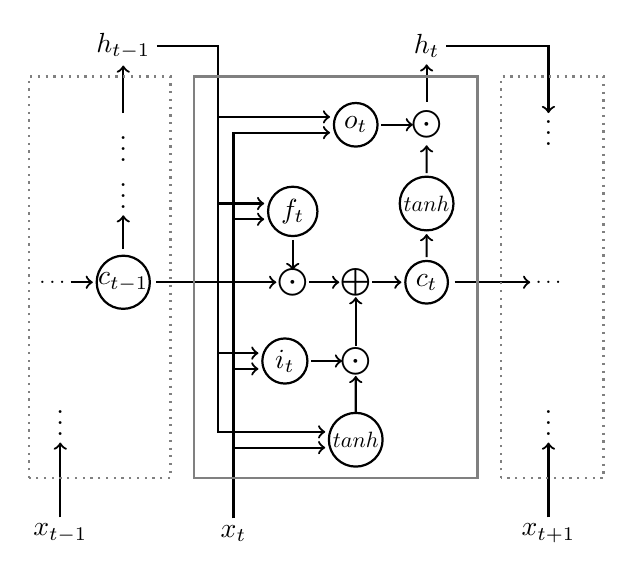
\begin{tikzpicture}[auto, thick, node distance=1cm, align=center, inner sep=2]

\draw
    (2.2,0) node [name=input] {$x_t$};
\coordinate[above=of input] (p1);
\draw
    node [right=1.2cm of p1, circle, draw, name=input activation, inner sep=1, scale=0.8] {$tanh$}
    node [above of=input activation, name=input multiplication] {$\bigodot$}
    node [above of=input multiplication, name=addition] {$\bigoplus$}
    node [right of=addition, circle, draw, name=memory, node distance=0.9cm] {$c_t$}
    node [above of=memory, circle, draw, name=output activation, inner sep=1, scale=0.8] {$tanh$}
    node [above of=output activation, name=output multiplication] {$\bigodot$}
    node [above of=output multiplication, name=output] {$h_t$}
    
    node[left of=input multiplication, circle, draw, name=input gate, node distance=0.9cm] {$i_t$}
    node[left of=addition, name=memory multiplication, node distance=0.8cm] {$\bigodot$}
    node[above of=memory multiplication, circle, draw, name=forget gate, node distance=0.9cm] {$f_t$}
    node[left of=output multiplication, circle, draw, name=output gate, node distance=0.9cm] {$o_t$}

;

\coordinate (prev output x) at (0.8,0);
\draw
    (0,0) node [name=prev input] {$x_{t-1}$}
    node [above of=prev input, node distance=1.5cm, name=input ellipsis] {$\vdots$}
    (prev output x |- output) node [name=prev output] {$h_{t-1}$}
    (prev output.south |- memory multiplication) node [circle, draw, name=prev memory, inner sep=0] {$c_{t-1}$}
    node [left of=prev memory, node distance=0.9cm, name=memory ellipsis in, scale=0.8] {$\ldots$}
    node [above of=prev memory, node distance=1.2cm, name=memory ellipsis out] {$\vdots$}

    node [below of=prev output, node distance=1.2cm, name=output ellipsis] {$\vdots$}
;

\draw
    (6.2,0) node [name=next input] {$x_{t+1}$}
    node [above of=next input, node distance=1.5cm, name=next input ellipsis] {$\vdots$}
    (next input |- memory) node [name=next memory ellipsis, scale=0.8] {$\ldots$}
    (next input |- output) node [yshift=-1cm, node distance=3.8cm, name=next output ellipsis] {$\vdots$}
;

\coordinate (p2) at (p1 |- input gate);
\coordinate (p3) at (p2 |- forget gate);
\coordinate (p4) at (p3 |- output gate);
\coordinate (p5) at ([xshift=-0.2cm]p4 |- prev output);


\draw[->] (prev input) -- (input ellipsis);
\draw[->, shorten >=1pt] (memory ellipsis in) -- (prev memory);
\draw[->, shorten <=2pt] (prev memory) -- (memory ellipsis out);
\draw[->] (output ellipsis) -- (prev output);

\draw[->, shorten <=2pt, shorten >=-2pt] (prev memory) -- (memory multiplication);

\draw[->, shorten >=1pt] (prev output) -- (p5) -- ([yshift=0.1cm, xshift=-0.2cm]p4) -- ([yshift=0.1cm]output gate.west);
\draw[->, shorten >=1pt] ([yshift=0.1cm, xshift=-0.2cm]p4) -- ([yshift=0.1cm, xshift=-0.2cm]p3) -- ([yshift=0.1cm]forget gate.west);
\draw[->, shorten >=1pt] ([yshift=0.1cm, xshift=-0.2cm]p3) -- ([yshift=0.1cm, xshift=-0.2cm]p2) -- ([yshift=0.1cm]input gate.west);
\draw[->, shorten >=1pt] ([yshift=0.1cm, xshift=-0.2cm]p2) -- ([yshift=0.1cm, xshift=-0.2cm]p1) -- ([yshift=0.1cm]input activation.west);


\draw[->, shorten >=1pt] (input) -- ([yshift=-0.1cm]p1) -- ([yshift=-0.1cm]input activation.west);
\draw[->, shorten >=1pt] ([yshift=-0.1cm]p1) -- ([yshift=-0.1cm]p2) -- ([yshift=-0.1cm]input gate.west);
\draw[->, shorten >=1pt] ([yshift=-0.1cm]p2) -- ([yshift=-0.1cm]p3) -- ([yshift=-0.1cm]forget gate.west);
\draw[->, shorten >=1pt] ([yshift=-0.1cm]p3) -- ([yshift=-0.1cm]p4) -- ([yshift=-0.1cm]output gate.west);
\draw[->, shorten >= -2pt] (input activation) -- (input multiplication);
\draw[->, shorten <=-2pt, shorten >=-2pt] (input multiplication) -- (addition);
\draw[->, shorten >=1pt, shorten <= -2pt] (addition) -- (memory);
\draw[->, shorten >=1pt, shorten <=1pt] (memory) -- (output activation);
\draw[->, shorten <=1pt] (output activation) -- (output multiplication);
\draw[->, shorten <=1pt] (output multiplication) -- (output);

\draw[->, shorten <=1pt, shorten >=-3pt] (input gate) -- (input multiplication);
\draw[->, shorten <=-2pt, shorten >= -2pt] (memory multiplication) -- (addition);
\draw[->, shorten <=1pt, shorten >=-3pt] (forget gate) -- (memory multiplication);
\draw[->, shorten <=1pt, shorten >=-3pt] (output gate) -- (output multiplication);

%% Boxes

\draw[->] (output) -- (next output ellipsis |- output) -- ([yshift=-0.2cm]next output ellipsis.north);
\draw[->, shorten <= 2pt] (memory) -- (next memory ellipsis);
\draw[->] (next input) -- (next input ellipsis);

\draw[gray] (1.7,0.7) rectangle (5.3,5.8);

\draw[dotted, gray] (-0.4,0.7) rectangle (1.4,5.8);

\draw[dotted, gray] (5.6,0.7) rectangle (6.9,5.8);

\end{tikzpicture}
    \caption{schematic model of an LSTM-cell. $\bigodot$ stands for element-wise multiplication and $\bigoplus$ for vector addition.}
    \label{fig:lstm_cell}

\end{figure}
%
\subsection{Basic Model}
\label{subsec:basic_model}
Now let us turn to the details of the model implementation.  We begin with the basic formulation.

Let $B_{open}$ and $B_{close}$ be the sets of opening and closing brackets and $B = B_{open} \cup B_{close}$ the set of all brackets. Given the beginning of a sentence $w_1, w_2, ..., w_{k-1}, w_k$ with $w_1, ..., w_{k-1} \in B$ and $w_k \in B_{close}$, the LSTMs tries approximate the function:
%
\begin{align*}
  F \colon B^{k-1} &\to B_{close}\\
  w_1, w_2, ..., w_{k-1} &\mapsto w_k.
  \label{eq:brackets_task_definition}
\end{align*}
%
The substring (clause) between the corresponding opening bracket of $w_i$ and $w_i$ will be referred to as the \emph{relevant clause} in the remainder of this paper. Likewise, by \emph{distance} we denote the number of characters of the relevant clause. Note that this distance is always a multiple of 2, since the relevant clause is well-balanced. The \emph{depth} at a certain position $i$ is the number of unclosed brackets in the first $i$ characters. The \emph{embedded depth} of a sentence is the maximum \emph{depth} when processing the relevant clause.

%Note that since a bracket pair consists of 2 characters, distances are always even. We denote \emph{odd distances} as ${2,6,10,14,...}$ and \emph{even distances} as ${4,8,12,16,...}$.

To read the input characters, an embedding layer with 5 output dimensions precedes the LSTM. Together they build the encoder, which will read the input sequentially. The decoder, mapping the internal representation to a probability of predicting \verb|}| or \verb|]| is a dense layer with one output variable.

\begin{figure*}[ht]
    \centering
        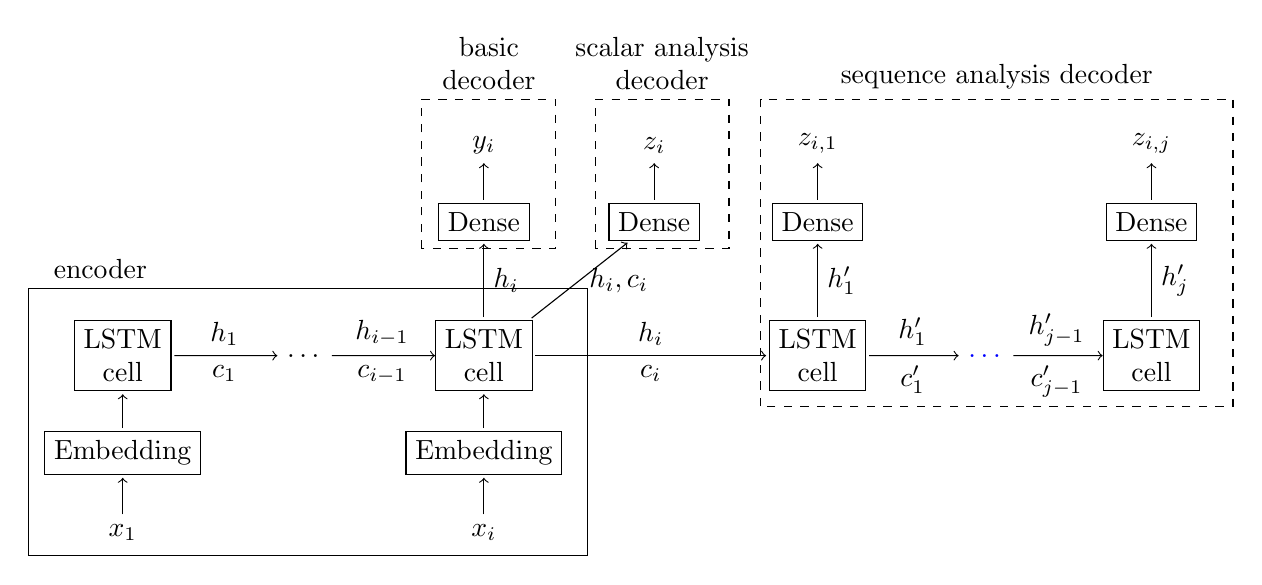
\begin{tikzpicture}[node distance=1.7cm, every text node part/.style={align=center}]
    \node (input1) at (0,0) {$x_1$};
    \node[above=0.5cm of input1, draw] (embedding1) {Embedding};
    \node[above=0.5cm of embedding1, draw] (lstm1) {LSTM \\ cell};

    \node[right=4cm of input1] (input3) {$x_i$};
    \node[above=0.5cm of input3, draw] (embedding3) {Embedding};
    \node[above=0.5cm of embedding3, draw] (lstm3) {LSTM \\ cell};
    \node[above of=lstm3, draw] (dense3) {Dense};
    \node[above=0.5cm of dense3] (output3) {$y_i$};
    
    \node[right=1cm of dense3, draw] (dense4) {Dense};
    \node[above=0.5cm of dense4] (output4) {$z_i$};
    
    \node[right=3cm of lstm3, draw] (lstm5) {LSTM \\ cell};
    \node[above of=lstm5, draw] (dense5) {Dense};
    \node[above=0.5cm of dense5] (output5) {$z_{i,1}$};

    \node[right=3cm of lstm5, draw] (lstm6) {LSTM \\ cell};
    \node[above of=lstm6, draw] (dense6) {Dense};
    \node[above=0.5cm of dense6] (output6) {$z_{i,j}$};
    
    \draw[->, shorten >= 1pt] (input1) -- (embedding1);
    \draw[->, shorten >= 1pt, shorten <= 1pt] (embedding1) -- (lstm1);

    
    \node (lstm dots) at ($(lstm1)!0.5!(lstm3)$) {$\ldots$};
    
    \draw[->, shorten <= 1pt] (lstm1) -- node[above]{$h_1$} node[below]{$c_1$} ++ (lstm dots);
    \draw[->, shorten <= 1pt] (lstm dots) -- node[above]{$h_{i-1}$} node[below]{$c_{i-1}$} ++ (lstm3);

    \draw[->, shorten >= 1pt] (input3) -- (embedding3);
    \draw[->, shorten >= 1pt, shorten <= 1pt] (embedding3) -- (lstm3);
    \draw[->, shorten >= 1pt, shorten <= 1pt] (lstm3) -- node[right] {$h_i$} ++ (dense3);
    \draw[->, shorten <= 1pt] (dense3) -- (output3);
    
    \draw[->, shorten <= 1pt, shorten >= 1pt] (lstm3) -- node[right] {$h_i, c_i$} ++ (dense4);
    \draw[->, shorten <= 1pt] (dense4) -- (output4);
    
    \draw[->, shorten <= 1pt, shorten >= 1pt] (lstm3) -- node[above] {$h_i$} node[below] {$c_i$} ++ (lstm5);
    
    \node[blue] (lstm dots analysis) at ($(lstm5)!0.5!(lstm6)$) {$\ldots$};
    
    \draw[->, shorten <= 1pt] (lstm5) -- node[above]{$h'_1$} node[below]{$c'_1$} ++ (lstm dots analysis);
    \draw[->, shorten <= 1pt] (lstm dots analysis) -- node[above]{$h'_{j-1}$} node[below]{$c'_{j-1}$} ++ (lstm6);
    \draw[->, shorten <= 1pt, shorten >= 1pt] (lstm5) -- node[right] {$h'_1$} ++ (dense5);
    \draw[->, shorten <= 1pt, shorten >= 1pt] (lstm6) -- node[right] {$h'_j$} ++ (dense6);
    \draw[->, shorten <= 1pt] (dense5) -- (output5);
    \draw[->, shorten <= 1pt] (dense6) -- (output6);
    
    \draw (-1.2,-0.3) rectangle (5.9,3.1);
    \draw (-1,3.1) node[anchor=south west] {encoder};
    
    \draw[dashed] (3.8, 3.6) rectangle (5.5, 5.5);
    \draw (4.65,5.5) node[anchor=south] {basic \\ decoder};
    
    \draw[dashed] (6, 3.6) rectangle (7.7, 5.5);
    \draw (6.85, 5.5) node[anchor=south] {scalar analysis \\ decoder};
    
    \draw[dashed] (8.1, 1.6) rectangle (14.1, 5.5);
    \draw (11.1, 5.5) node[anchor=south] {sequence analysis decoder};
    
    \end{tikzpicture}
    \caption{Network architecture of the model. The basic end-to-end model consists of the encoder and the basic decoder. The analysis model fixes the weights for the encoder and uses the scalar (if $z_i$ is a scalar) or sequence analysis decoder (if $z_i$ is a sequence).}
    \label{fig:lstm_architecture}
\end{figure*}

We have compared different initialization methods. It turns out that the initialization of the model is crucial to avoid bad local minima. The following initialization method results in consistently good solutions: To initialize the weights, the model is trained with sentences of length 50 and only afterwards on the actual corpus with sentence length 100.

For backpropagation, the Adam \cite{kingma2014adam} optimizer was used. Furthermore, to ensure faster and more consistent convergence, at the beginning of the training, the batch size is gradually increased, which has a similar effect as reducing the learning rate \cite{smith2017don}. In all experiments (and for all models), the corpus is split into 50\% training sentences and 50\% test sentences. The reported results always refer to the results on the test set.

\subsection{Analysis Model}

The analysis model is used to analyze what information is stored in the internal representation of the LSTM. In a Push-Down-Automaton model, this internal representation would conceptually correspond to the entire stack.

To analyze the internal representation $[h_i, c_i]$ of the LSTM after having read the input or part of it, we use a method already developed by \citeauthor{shi2016does} \shortcite{shi2016does} and \citeauthor{belinkov2017neural} \shortcite{belinkov2017neural}: After having trained the basic model, the weights of the encoder are fixed and the labels (previously $y$) are replaced by some feature $z_i$ of the input $x_1,\ldots, x_i$.

This feature $z_i$ can either be a scalar or a vector. If $z_i$ is a scalar, a dense layer (scalar analysis decoder) is trained to predict $z_i$. On the other hand, if $z_i$ is a vector (sequence analysis decoder), another LSTM is trained to predict $z_{i,1},\ldots,z_{i,j}$.\\

Analyzing the performance of the analysis network shows us how accurately a feature $z_i$ is preserved in $[h_i, c_i]$. One can assume that the LSTM uses its limited memory ``efficiently'' and therefore discards irrelevant information. Hence, the performance of the analysis decoder shows whether $z_i$ is contained in the information that is relevant for the original classification task.

To begin, two of the experiments which were conducted are presented in the following section to test the trained model performance. For the first experiment $z_i$ is the \emph{depth} (nesting level) after $i$ characters.

\textbf{Example:} For the sequence \verb|{[{}[[]|, $z$ is $(1,2,3,2,3,4,3)$.\\

For the second experiment we note that theoretically, at any time $t$, no information about a closed clause in $w_1,\ldots, w_t$ has to be stored, since it is irrelevant for any eventual future prediction of $w_{t+1}, w_{t+2},\ldots$. 
When reading from left to right, as soon as a closing bracket is processed, the corresponding clause becomes irrelevant. Therefore, the relevant information is simply the list of bracket types of unclosed clauses. In this experiment we investigate how well the previous characters are preserved in the intermediate representation and evaluate if this correlates with the recovered characters being relevant or not.

\textbf{Example:} after having processed \verb|{[{}][|, only the first and the last characters are relevant, since they are the only ones that could matter for a future classification task. On the other hand, the sub-string \verb|[{}]| is irrelevant. In this example we would evaluate whether the first and last character are better preserved in the intermediate state than the irrelevant sub-string.

To set up the experiment, we set $z_{i,k}$ to be equal to $x_{i-k+1}$, corresponding to predicting the previous characters of a given intermediate state.

\subsection{Varying hidden units}
\label{subsec:varying_hidden_units}

The basic model is evaluated with $2,4,6,...,50$ hidden units. The error rate with 50 hidden units is 0.38\% and an error rate of 1\% is reached around 20 hidden units.  Thus, the error seems to converge with increasing hidden units to a fairly small value. As a result, in all further experiments, the maximum number of hidden units the models are tested against was set to 50.

\setlength\figureheight{4cm}
\setlength\figurewidth{\linewidth}
\begin{figure}[ht]
    % This file was created by matplotlib2tikz v0.6.17.
\begin{tikzpicture}

\definecolor{color0}{rgb}{0.12156862745098,0.466666666666667,0.705882352941177}

\begin{axis}[
xlabel={units},
ylabel={error rate},
xmin=-0.4, xmax=52.4,
ymin=0.00272669964390025, ymax=0.388158976867021,
ymode=log,
width=\figurewidth,
height=\figureheight,
tick align=outside,
tick pos=left,
x grid style={lightgray!92.02614379084967!black},
y grid style={lightgray!92.02614379084967!black}
]
\addplot [very thick, black, forget plot]
table {%
2 0.309834
4 0.131702
6 0.0495
8 0.0313
10 0.02149
12 0.0138779999999999
14 0.014466
16 0.011456
18 0.011836
20 0.01105
22 0.00742200000000004
24 0.00552600000000003
26 0.011324
28 0.00360400000000005
30 0.00609000000000004
32 0.004112
34 0.00595000000000001
36 0.00451999999999997
38 0.00400800000000001
40 0.00564799999999999
42 0.006212
44 0.00341599999999997
46 0.00486200000000003
48 0.00432600000000005
50 0.00384399999999996
};
\end{axis}

\end{tikzpicture}%
    \caption{Overall error rate of the basic model with respect to the number of hidden units of the LSTM.}%
    \label{fig:varying_units_results}%
\end{figure}

\subsection{Memory demand}
\label{subsec:memory_demand}

In this section we evaluate how ``difficult'' sentences can be with respect to the memory demand of the model, while still reaching an error tolerance of 5\%. We have to work with tolerances, because 100\% accuracy is not reached. Since it can be challenging measuring how difficult a sentence is to predict, we use the \emph{distance} and the \emph{embedded depth} of a sentence as defined above as metrics.

\setlength\figureheight{5cm}
\setlength\figurewidth{0.48\textwidth}
\begin{figure*}[ht]
    % This file was created by matplotlib2tikz v0.6.17.
\begin{tikzpicture}

\definecolor{color0}{rgb}{0.12156862745098,0.466666666666667,0.705882352941177}

\begin{axis}[
xlabel={hidden units},
ylabel={distance},
xmin=-1.45, xmax=52.45,
ymin=-20.802587179018, ymax=100.597830773957,
width=\figurewidth,
height=\figureheight,
tick align=outside,
tick pos=left,
x grid style={lightgray!92.02614379084967!black},
y grid style={lightgray!92.02614379084967!black}
]
\addplot [very thick, gray, dashed, forget plot]
table {%
1 -15.2843863629737
1.4949494949495 -3.94075808103901
1.98989898989899 4.1274883379046
2.48484848484848 10.3940457953906
2.97979797979798 15.5184894738201
3.47474747474747 19.8536455124497
3.96969696969697 23.6105125561782
4.46464646464647 26.9253708075226
4.95959595959596 29.8913650243448
5.45454545454546 32.5749837904557
5.94949494949495 35.0253508303714
6.44444444444444 37.2797906080873
6.93939393939394 39.3673286210571
7.43434343434343 41.3109828660492
7.92929292929293 43.129315234753
8.42424242424243 44.8375123408373
8.91919191919192 46.4481573049852
9.41414141414142 47.9717928239192
9.90909090909091 49.417339794359
10.4040404040404 50.7924137959027
10.8989898989899 52.1035679524578
11.3939393939394 53.3564818131212
11.8888888888889 54.5561100396219
12.3838383838384 55.7068007463889
12.8787878787879 56.812390635396
13.3737373737374 57.8762821806949
13.8686868686869 58.9015067795721
14.3636363636364 59.8907768249906
14.8585858585859 60.8465289527432
15.3535353535354 61.7709601994918
15.8484848484848 62.6660584220042
16.3434343434343 63.533628037042
16.8383838383838 64.3753119199611
17.3333333333333 65.1926101300394
17.8282828282828 65.9868959988224
18.3232323232323 66.7594300149295
18.8181818181818 67.5113718578532
19.3131313131313 68.2437908691913
19.8080808080808 68.957675198637
20.3030303030303 69.6539398210373
20.7979797979798 70.333433587715
21.2929292929293 70.9969454483795
21.7878787878788 71.6452099580086
22.2828282828283 72.2789121650987
22.7777777777778 72.8986919628477
23.2727272727273 73.5051479725595
23.7676767676768 74.0988410183493
24.2626262626263 74.6802972437022
24.7575757575758 75.2500109132899
25.2525252525253 75.8084469374343
25.7474747474747 76.3560431515272
26.2424242424242 76.8932123784037
26.7373737373737 77.4203442980101
27.2323232323232 77.9378071455759
27.7272727272727 78.4459492568276
28.2222222222222 78.9451004764848
28.7171717171717 79.4355734443031
29.2121212121212 79.9176647712193
29.7070707070707 80.3916561166812
30.2020202020202 80.8578151769584
30.6969696969697 81.3163965931191
31.1919191919192 81.7676427863818
31.6868686868687 82.2117847277047
32.1818181818182 82.6490426477279
32.6767676767677 83.0796266925323
33.1717171717172 83.5037375301023
33.6666666666667 83.9215669118738
34.1616161616162 84.3332981933016
34.6565656565657 84.7391068169815
35.1515151515152 85.1391607615167
35.6464646464647 85.5336209589987
36.1414141414141 85.9226416837032
36.6363636363636 86.3063709143483
37.1313131313131 86.6849506720443
37.6262626262626 87.058517335867
38.1212121212121 87.4272019378091
38.6161616161616 87.7911304387056
39.1111111111111 88.1504239865873
39.6060606060606 88.5051991587889
40.1010101010101 88.8555681890217
40.5959595959596 89.2016391805178
41.0909090909091 89.5435163062591
41.5858585858586 89.8812999972179
42.0808080808081 90.2150871194614
42.5757575757576 90.5449711409009
43.0707070707071 90.8710422884036
43.5656565656566 91.1933876959289
44.0606060606061 91.5120915442953
44.5555555555556 91.8272351931423
45.0505050505051 92.1388973056008
45.5454545454545 92.4471539661538
46.040404040404 92.7520787921258
46.5353535353535 93.0537430392123
47.030303030303 93.3522157014257
47.5252525252525 93.6475636058101
48.020202020202 93.9398515022483
48.5151515151515 94.2291421486653
49.010101010101 94.5154963919065
49.5050505050505 94.7989732445524
50 95.0796299579128
};
\addplot [very thick, black, mark=x, mark size=3, mark options={solid}, forget plot]
table {%
2 5
4 21
6 33
8 39
10 49
12 57
14 57
16 63
18 61
20 63
22 77
24 91
26 65
28 91
30 83
32 89
34 89
36 87
38 93
40 85
42 83
44 91
46 87
48 91
50 91
};
\end{axis}

\end{tikzpicture}\qquad
    % This file was created by matplotlib2tikz v0.6.17.
\begin{tikzpicture}

\definecolor{color0}{rgb}{0.12156862745098,0.466666666666667,0.705882352941177}

\begin{axis}[
xlabel={hidden units},
ylabel={embedded depth},
xmin=-1.45, xmax=52.45,
ymin=1.6079327425331, ymax=19.4243492868153,
width=\figurewidth,
height=\figureheight,
tick align=outside,
tick pos=left,
x grid style={lightgray!92.02614379084967!black},
y grid style={lightgray!92.02614379084967!black}
]
\addplot [very thick, gray, dashed, forget plot]
table {%
1 2.41776985818229
1.4949494949495 4.08253189114937
1.98989898989899 5.2666072131758
2.48484848484848 6.1862712460006
2.97979797979798 6.93832156569536
3.47474747474747 7.57453803900771
3.96969696969697 8.12588629036611
4.46464646464647 8.61236645564922
4.95959595959596 9.04764822259756
5.45454545454546 9.4414892866506
5.94949494949495 9.80109892066709
6.44444444444444 10.1319547680444
6.93939393939394 10.4383165369593
7.43434343434343 10.7235622900692
7.92929292929293 10.990416123384
8.42424242424243 11.2411067856973
8.91919191919192 11.4774809437939
9.41414141414142 11.7010858170284
9.90909090909091 11.9132306135122
10.4040404040404 12.115032976336
10.8989898989899 12.3074546252961
11.3939393939394 12.4913290765713
11.8888888888889 12.6673834637143
12.3838383838384 12.8362559049388
12.8787878787879 12.9985094648675
13.3737373737374 13.1546434819375
13.8686868686869 13.3051028363042
14.3636363636364 13.4502855918593
14.8585858585859 13.590549343074
15.3535353535354 13.7262165214606
15.8484848484848 13.8575788598217
16.3434343434343 13.9849011697718
16.8383838383838 14.1084245555192
17.3333333333333 14.2283691619479
17.8282828282828 14.3449365357023
18.3232323232323 14.4583116628862
18.8181818181818 14.568664735112
19.3131313131313 14.6761526862326
19.8080808080808 14.7809205345836
20.3030303030303 14.8831025595461
20.7979797979798 14.9828233363811
21.2929292929293 15.0801986493413
21.7878787878788 15.1753362998468
22.2828282828283 15.2683368238724
22.7777777777778 15.3592941305161
23.2727272727273 15.4482960719179
23.7676767676768 15.5354249531985
24.2626262626263 15.6207579898373
24.7575757575758 15.7043677188605
25.2525252525253 15.7863223693243
25.7474747474747 15.866686196837
26.2424242424242 15.945519786228
26.7373737373737 16.022880325935
27.2323232323232 16.0988218572236
27.7272727272727 16.173395500959
28.2222222222222 16.2466496643132
28.7171717171717 16.3186302295016
29.2121212121212 16.3893807263907
29.7070707070707 16.4589424906048
30.2020202020202 16.5273548085674
30.6969696969697 16.594655050754
31.1919191919192 16.6608787942859
31.6868686868687 16.7260599358736
32.1818181818182 16.7902307960055
32.6767676767677 16.853422215186
33.1717171717172 16.9156636429381
33.6666666666667 16.9769832202147
34.1616161616162 17.0374078557961
34.6565656565657 17.0969632971912
35.1515151515152 17.1556741965127
35.6464646464647 17.2135641717449
36.1414141414141 17.2706558637881
36.6363636363636 17.3269709896227
37.1313131313131 17.3825303919055
37.6262626262626 17.4373540852827
38.1212121212121 17.4914612996764
38.6161616161616 17.5448705207782
39.1111111111111 17.5975995279651
39.6060606060606 17.6496654298302
40.1010101010101 17.7010846975073
40.5959595959596 17.751873195952
41.0909090909091 17.802046213326
41.5858585858586 17.8516184886235
42.0808080808081 17.9006042376619
42.5757575757576 17.9490171775543
43.0707070707071 17.9968705497662
43.5656565656566 18.0441771418558
44.0606060606061 18.0909493079859
44.5555555555556 18.1371989882902
45.0505050505051 18.1829377271699
45.5454545454545 18.22817669059
46.040404040404 18.2729266824419
46.5353535353535 18.3171981600301
47.030303030303 18.3610012487406
47.5252525252525 18.4043457559401
48.020202020202 18.4472411841569
48.5151515151515 18.4896967435845
49.010101010101 18.531721363951
49.5050505050505 18.5733237057927
50 18.6145121711661
};
\addplot [very thick, black, mark=x, mark size=3, mark options={solid}, forget plot]
table {%
2 3
4 6
6 9
8 11
10 12
12 13
14 14
16 15
18 15
20 15
22 16
24 17
26 14
28 18
30 17
32 18
34 18
36 17
38 18
40 17
42 16
44 18
46 17
48 18
50 18
};
\end{axis}

\end{tikzpicture}
    \caption{\emph{Distances} (left figure) and \emph{embedded depth} (right figure) that can be predicted with a given number of hidden units and 5\% error tolerance. The dashed line is a logarithmic approximation.}%
    \label{fig:memory_demand}%
\end{figure*}

The resulting values (figure \ref{fig:memory_demand}) demonstrate that memory demand grows exponentially with respect to the \emph{distance} of sentences that can be predicted. The same behaviour can be observed with respect to the \emph{embedded depth}. 

\subsection{Generalization}
\label{subsec:generalization}

To evaluate the model's generalization performance, training was done only on a systematically chosen subset of sentences (in-sample). To avoid adding additional nuisance variables in this selection, the training sentences are selected according to one of the following rules:

\begin{samepage}
\begin{description}
    \item[regular interpolation:] the sentence has \emph{distance} $2,6,10,14,\ldots$ / odd \emph{embedded depth}.
    \item[random interpolation:] the \emph{distance} / \emph{embedded depth} of the relevant clause belongs to a set $D$. $D$ is a random subset consisting of half of all \emph{distances} / \emph{embedded depths} present in the corpus.
    \item[extrapolation:] the \emph{distance} / \emph{embedded depth} of the relevant clause is smaller than a certain threshold (11 for \emph{distance} and 13 for \emph{embedded depth}).
\end{description}
\end{samepage}

\begin{figure}
    \centering
    % This file was created by matplotlib2tikz v0.6.17.
\begin{tikzpicture}

%\definecolor{black}{rgb}{0.83921568627451,0.152941176470588,0.156862745098039}
%\definecolor{gray}{rgb}{0.12156862745098,0.466666666666667,0.705882352941177}

\begin{axis}[
xlabel={distance},
ylabel={error rate},
xmin=-3.9, xmax=103.9,
ymin=-0.0258774989587672, ymax=0.573983033689666,
width=\figurewidth,
height=\figureheight,
tick align=outside,
tick pos=left,
ytick = {0,0.1,0.2,0.3,0.4,0.5},
x grid style={lightblack!92.02614379084967!gray},
y grid style={lightblack!92.02614379084967!gray}
]
\addplot [very thick, gray, opacity=0.15, forget plot]
table {%
1 0.073402654261869
3 0.0546071944564587
7 0.0477555248618785
13 0.0616718785260647
17 0.0842992190711056
21 0.119164851813275
23 0.135215229293284
27 0.173757371524853
33 0.235820548582055
35 0.2543391188251
41 0.304920257889379
45 0.325753529187333
49 0.345445196674951
51 0.358375269590223
53 0.366676166049207
55 0.360853805879984
57 0.380775532495904
65 0.38206302929335
67 0.410194540793244
69 0.400998595724762
71 0.408602150537634
77 0.421887235708692
79 0.429572976418101
93 0.45862676056338
99 0.436860068259386
};
\addplot [very thick, gray, opacity=0.15, forget plot]
table {%
1 0.0748620422310393
3 0.0142637599271168
7 0.0100828729281768
13 0.0248557335826429
17 0.0542540073982737
21 0.103778051320898
23 0.133859058717163
27 0.196345829823083
33 0.273535564853556
35 0.291904357324918
41 0.336613505259586
45 0.361694009919878
49 0.385637158282629
51 0.389288281811646
53 0.400208986415883
55 0.400020136931132
57 0.412233752048061
65 0.417881438289602
67 0.427838938320012
69 0.418630051490092
71 0.425067204301075
77 0.435591229444009
79 0.458466114297854
93 0.470070422535211
99 0.508532423208191
};
\addplot [semithick, gray, opacity=0.15, forget plot]
table {%
1 0.221023167784011
3 0.164640599261966
7 0.17396408839779
13 0.231761178632451
17 0.276448828606658
21 0.312091657986933
23 0.317544828971822
27 0.322714827295703
33 0.342689446768945
35 0.356535987377109
41 0.395045809297591
45 0.419305608546356
49 0.434998714542806
51 0.437724658519051
53 0.443336183148095
55 0.452879581151832
57 0.459858001092299
65 0.475912814105234
67 0.469310812848741
69 0.482758620689655
71 0.479838709677419
77 0.496084573218481
79 0.485234756745273
93 0.499119718309859
99 0.476109215017065
};
\addplot [semithick, gray, opacity=0.15, forget plot]
table {%
1 0.074041136498381
3 0.0523157904423606
7 0.0697686464088397
13 0.141655114607176
17 0.199712289354706
21 0.245099895843197
23 0.276859711688181
27 0.316975568660489
33 0.361866573686657
35 0.366549338511955
41 0.384526637258229
45 0.416863792445631
49 0.421887051161196
51 0.432692307692308
53 0.439251448655837
55 0.447845348368909
57 0.445548880393228
65 0.458420102734972
67 0.480168903634444
69 0.455921360586675
71 0.468918010752688
77 0.487274862960063
79 0.484384958572339
93 0.493397887323944
99 0.525597269624573
};
\addplot [semithick, gray, opacity=0.15, forget plot]
table {%
1 0.106210379896931
3 0.0642053245235444
7 0.0728418508287293
13 0.111480060608014
17 0.156185778873818
21 0.204242022535745
23 0.226229343512984
27 0.271008845829823
33 0.328509995351
35 0.339665007889307
41 0.386291143535799
45 0.403739030904235
49 0.426943182792013
51 0.431883537023724
53 0.441816281941674
55 0.449859041482078
57 0.457018022938285
65 0.474663334721644
67 0.468707585582868
69 0.465595256670307
71 0.468581989247312
77 0.485708692247455
79 0.477161674102401
93 0.494278169014085
99 0.479522184300341
};
\addplot [semithick, gray, opacity=0.15, forget plot]
table {%
1 0.0569047293291376
3 0.0439139757240008
7 0.0483770718232044
13 0.0921048389696637
17 0.134936292642828
21 0.179481109743395
23 0.193731478225928
27 0.228675231676495
33 0.27463970246397
35 0.292571914067241
41 0.333288089582626
45 0.354292254864556
49 0.370468763390179
51 0.371046010064702
53 0.375795573287736
55 0.380789367700362
57 0.381540141998908
65 0.413022351797862
67 0.413059870306138
69 0.411452644718365
71 0.407762096774194
77 0.417971808927173
79 0.432122370936903
93 0.449383802816901
99 0.493174061433447
};
\addplot [semithick, gray, opacity=0.15, forget plot]
table {%
1 0.0312172207780362
3 0.0149355370075552
7 0.00965124309392262
13 0.0181501660272736
17 0.0350184956843403
21 0.0635356500331408
23 0.0838314330202421
27 0.128738416175232
33 0.199848907484891
35 0.225573491928632
41 0.299355276552426
45 0.33918351774132
49 0.367469363270203
51 0.375988497483825
53 0.381305215161015
55 0.400020136931132
57 0.408956854178045
65 0.426766625017354
67 0.431759915548183
69 0.432672803869558
71 0.433131720430108
77 0.448903680501175
79 0.460378160186956
93 0.493397887323944
99 0.491467576791809
};
\addplot [semithick, gray, opacity=0.15, forget plot]
table {%
1 0.0378984813243946
3 0.0302299686197282
7 0.0327866022099448
13 0.0561913665817725
17 0.0762433210028771
21 0.104109459331503
23 0.11190918679994
27 0.140690817186184
33 0.191364481636448
35 0.215074644981187
41 0.273566338649474
45 0.302251049217856
49 0.334475961950467
51 0.340402588066139
53 0.346632468889522
55 0.348469593233991
57 0.367012561441835
65 0.38456198806053
67 0.394661438697029
69 0.401778748634732
71 0.408938172043011
77 0.431284259984338
79 0.420437646059061
93 0.470070422535211
99 0.450511945392492
};
\addplot [semithick, gray, opacity=0.15, forget plot]
table {%
1 0.0705864915401103
3 0.021349627761878
7 0.0227555248618785
13 0.0687643057480899
17 0.0951500205507604
21 0.121910803901146
23 0.131900145662766
27 0.157224094355518
33 0.204614132961413
35 0.219808229154024
41 0.261350525958602
45 0.299046165585654
49 0.319393264204302
51 0.328720345075485
53 0.335803172793768
55 0.344844945630286
57 0.355106499180776
65 0.373871997778703
67 0.396772734127583
69 0.387267904509284
71 0.393145161290323
77 0.411902897415818
79 0.41427660930529
93 0.454665492957746
99 0.501706484641638
};
\addplot [semithick, gray, opacity=0.15, forget plot]
table {%
1 0.0545731290190177
3 0.0387422124472011
7 0.0377244475138122
13 0.0804023340533222
17 0.119194410193177
21 0.166887605340403
23 0.182831885077101
27 0.222514743049705
33 0.270339377033938
35 0.283286806651293
41 0.329894808279606
45 0.34017550553224
49 0.356243037106864
51 0.360801581595974
53 0.372185807922485
55 0.379480467176802
57 0.380666302566903
65 0.401360544217687
67 0.412004222590861
69 0.420658449056015
71 0.403729838709677
77 0.424040720438528
79 0.4282982791587
93 0.462588028169014
99 0.484641638225256
};
\addplot [semithick, gray, opacity=0.15, forget plot]
table {%
1 0.0885552059105212
3 0.0593648485740841
7 0.0499827348066298
13 0.0705374125535961
17 0.0908754623921085
21 0.124798787993561
23 0.137274599427395
27 0.18270850884583
33 0.248430962343096
35 0.265444835538293
41 0.327790973871734
45 0.34765356734071
49 0.376981746507841
51 0.381200575125809
53 0.386244894081885
55 0.385219492549336
57 0.391589295466958
65 0.411078717201166
67 0.420298597496607
69 0.431736620377594
71 0.422883064516129
77 0.427173061863743
79 0.454004673889951
93 0.496919014084507
99 0.472696245733788
};
\addplot [semithick, gray, opacity=0.15, forget plot]
table {%
1 0.0907214849272586
3 0.0643157536326576
7 0.0708908839779006
13 0.0851413649698571
17 0.0893136046033703
21 0.100179907205757
23 0.116228841227585
27 0.170282224094356
33 0.279869827986983
35 0.310838694016264
41 0.377400746521887
45 0.405265165967188
49 0.425572028451453
51 0.434579439252336
53 0.438491498052627
55 0.446637132501007
57 0.444456581103222
65 0.471331389698737
67 0.471572915095762
69 0.481666406615697
71 0.472278225806452
77 0.481989036805012
79 0.483110261312938
93 0.501760563380282
99 0.510238907849829
};
\addplot [semithick, gray, opacity=0.15, forget plot]
table {%
1 0.148350207506727
3 0.160619139205094
7 0.223342541436464
13 0.332667075018537
17 0.395889847924373
21 0.429504781744153
23 0.441458636797428
27 0.457087194608256
33 0.46048349604835
35 0.463709188008253
41 0.468612147947065
45 0.481419305608546
49 0.485388636558403
51 0.491103522645579
53 0.485418447800893
55 0.47885622231172
57 0.499290005461496
65 0.489379425239484
67 0.501281857939979
69 0.488999843969418
71 0.478326612903226
77 0.496084573218481
79 0.503505417463352
93 0.495598591549296
99 0.520477815699659
};
\addplot [semithick, gray, opacity=0.15, forget plot]
table {%
1 0.0537864276918867
3 0.040794353391554
7 0.0457009668508287
13 0.115767755246784
17 0.17324290998767
21 0.227109175267494
23 0.249736300165754
27 0.294650379106992
33 0.341643421664342
35 0.351134846461949
41 0.387784187309128
45 0.405875619992369
49 0.421715656868626
51 0.418763479511143
53 0.423482473639213
55 0.429520741039066
57 0.430365920262152
65 0.441899208663057
67 0.455134972100739
69 0.450148229052894
71 0.440860215053763
77 0.435591229444009
79 0.459103462927555
93 0.482834507042254
99 0.486348122866894
};
\addplot [semithick, gray, opacity=0.15, forget plot]
table {%
1 0.125718292516076
3 0.0578096386207404
7 0.0522617403314917
13 0.0834327347754602
17 0.140402794903411
21 0.217640374964492
23 0.255964639107941
27 0.335930918281382
33 0.418874941887494
35 0.440769510862969
41 0.486868001357313
45 0.503243037008775
49 0.512126146199332
51 0.513389647735442
53 0.516576422532535
55 0.532118405155054
57 0.52605133806663
65 0.54671664584201
67 0.538380334791133
69 0.524418786082072
71 0.539314516129032
77 0.533281127642913
79 0.52836201402167
93 0.54137323943662
99 0.513651877133106
};
\addplot [semithick, gray, opacity=0.15, forget plot]
table {%
1 0.0572467733844119
3 0.0610672973395787
7 0.0717196132596685
13 0.103323769302685
17 0.130086313193588
21 0.162721333207083
23 0.177105831533477
27 0.217670598146588
33 0.275511390051139
35 0.294513897317636
41 0.349372242958941
45 0.369400991987791
49 0.391464564230011
51 0.397465851905104
53 0.399164054336468
55 0.406866693515908
57 0.401747678864009
65 0.427183118145217
67 0.437490574573971
69 0.442190669371197
71 0.426075268817204
77 0.439702427564605
79 0.46250265561929
93 0.507042253521127
99 0.537542662116041
};
\addplot [semithick, gray, opacity=0.15, forget plot]
table {%
1 0.104568568431614
3 0.066570347943718
7 0.070614640883978
13 0.113253167413521
17 0.14845869297164
21 0.174083893570685
23 0.191270279772967
27 0.222304128053917
33 0.279579265457927
35 0.293907027551887
41 0.335256192738378
45 0.352766119801602
49 0.376381866483846
51 0.389827462257369
53 0.385389949653273
55 0.388542086186065
57 0.393773894046969
65 0.403581840899625
67 0.420449404313075
69 0.410204400062412
71 0.414986559139785
77 0.420516836335161
79 0.446993838963246
93 0.474911971830986
99 0.511945392491468
};
\addplot [semithick, gray, opacity=0.15, forget plot]
table {%
1 0.0209273954485337
3 0.0181655884491152
7 0.018646408839779
13 0.0477126922208969
17 0.0743115495273325
21 0.0987122431587918
23 0.108041589231001
27 0.140743470935131
33 0.185495118549512
35 0.200631144556378
41 0.260128944689515
45 0.294009919877909
49 0.328477161710515
51 0.334831056793674
53 0.340552864063836
55 0.352094240837696
57 0.362424904423812
65 0.396223795640705
67 0.402352586336902
69 0.410204400062412
71 0.398185483870968
77 0.417188723570869
79 0.435096664542171
93 0.477112676056338
99 0.5
};
\addplot [semithick, gray, opacity=0.15, forget plot]
table {%
1 0.0958008391480822
3 0.0697175775534431
7 0.0924378453038674
13 0.149940359134724
17 0.195848746403617
21 0.241501751728056
23 0.260635893314581
27 0.305023167649537
33 0.354834960483496
35 0.365456972933608
41 0.402307431286054
45 0.417474246470813
49 0.43234210300797
51 0.430625449317038
53 0.433646812957158
55 0.44049536850584
57 0.453194975423266
65 0.453699847285853
67 0.465842256069974
69 0.467311593072242
71 0.460013440860215
77 0.454189506656225
79 0.470363288718929
93 0.472711267605634
99 0.472696245733788
};
\addplot [semithick, gray, opacity=0.15, forget plot]
table {%
1 0.0483935330870616
3 0.0264937837613995
7 0.021460635359116
13 0.0379122473322803
17 0.0581586518701191
21 0.0859767067512546
23 0.107137475513587
27 0.156644903117102
33 0.234309623430962
35 0.262531860662702
41 0.330030539531727
45 0.362151850438764
49 0.38837946696375
51 0.398544212796549
53 0.400778949368291
55 0.417438582360048
57 0.412342981977062
65 0.449812578092461
67 0.454682551651335
69 0.450304259634888
71 0.450772849462366
77 0.471613155833986
79 0.475249628213299
93 0.504401408450704
99 0.505119453924915
};
\addplot [semithick, gray, opacity=0.15, forget plot]
table {%
1 0.0831224061659142
3 0.057671602234349
7 0.0690089779005525
13 0.0921370772752184
17 0.124537607891492
21 0.178155477700975
23 0.201567130443518
27 0.259635636057287
33 0.321652719665272
35 0.332686005583202
41 0.378690193417034
45 0.395497901564288
49 0.415374068043534
51 0.416606757728253
53 0.421962572432792
55 0.424889246878776
57 0.429492080830147
65 0.44842426766625
67 0.458151108430101
69 0.455609299422687
71 0.445900537634409
77 0.450274079874706
79 0.468876141916295
93 0.494278169014085
99 0.488054607508532
};
\addplot [semithick, gray, opacity=0.15, forget plot]
table {%
1 0.0273977288274729
3 0.00828218318348717
7 0.00502417127071819
13 0.0109287855830298
17 0.022400328812166
21 0.0399583372786668
23 0.0570596212768095
27 0.103622577927548
33 0.177417480241748
35 0.205850224541813
41 0.279131319986427
45 0.316596718809615
49 0.34304567657897
51 0.347501797268152
53 0.366391184573003
55 0.371929118002416
57 0.377170944838886
65 0.408579758433986
67 0.410948574875584
69 0.428459978155719
71 0.425067204301075
77 0.448512137823023
79 0.43807095814744
93 0.480193661971831
99 0.494880546075085
};
\addplot [semithick, gray, opacity=0.15, forget plot]
table {%
1 0.0958863501619008
3 0.0785887159855337
7 0.0965987569060773
13 0.138527998968374
17 0.174352651048089
21 0.212669254805416
23 0.22683208599126
27 0.262794860994103
33 0.313284518828452
35 0.3334142493021
41 0.374211062097048
45 0.390309042350248
49 0.413574427971549
51 0.416247304097771
53 0.419207751496153
55 0.418244059605316
57 0.432113599126161
65 0.441760377620436
67 0.441109938169205
69 0.449368076142924
71 0.447916666666667
77 0.460649960845732
79 0.468876141916295
93 0.460387323943662
99 0.486348122866894
};
\addplot [semithick, gray, opacity=0.15, forget plot]
table {%
1 0.046244356273088
3 0.0317299640185152
7 0.0399516574585635
13 0.0884619104419871
17 0.134771886559803
21 0.190606950099422
23 0.208197297704556
27 0.243312973883741
33 0.288063691306369
35 0.306469231702877
41 0.35588734306074
45 0.375963372758489
49 0.392321535692861
51 0.400161754133717
53 0.403438776479529
55 0.411699556987515
57 0.420207536865101
65 0.438428432597529
67 0.445935756296185
69 0.442814791699173
71 0.452452956989247
77 0.46123727486296
79 0.45272997663055
93 0.47931338028169
99 0.5
};
\addplot [semithick, gray, opacity=0.15, forget plot]
table {%
1 0.112464085374196
3 0.0419998711660393
7 0.0368439226519337
13 0.0605757761372062
17 0.0967118783394986
21 0.144399204620775
23 0.169672007634738
27 0.23030749789385
33 0.303812180381218
35 0.325707003277097
41 0.368917543264337
45 0.390843189622282
49 0.40371925614877
51 0.402408339324227
53 0.408568443051202
55 0.418344744260975
57 0.415838339705079
65 0.437456615299181
67 0.445784949479716
69 0.452800748946794
71 0.442204301075269
77 0.449099451840251
79 0.456341618865519
93 0.488996478873239
99 0.546075085324232
};
\addplot [semithick, gray, opacity=0.15, forget plot]
table {%
1 0.0902825283896566
3 0.0553433885172131
7 0.0531767955801105
13 0.0885263870530965
17 0.11960542540074
21 0.154104724931351
23 0.17087749259129
27 0.207297809604044
33 0.263249651324965
35 0.280009709916252
41 0.326705123854768
45 0.344219763449065
49 0.363441597394807
51 0.369069015097052
53 0.377410468319559
55 0.373137333870318
57 0.377498634625888
65 0.388310426211301
67 0.39933645000754
69 0.406615696676549
71 0.39801747311828
77 0.411119812059515
79 0.424686636923731
93 0.463468309859155
99 0.447098976109215
};
\addplot [semithick, gray, opacity=0.15, forget plot]
table {%
1 0.0202832124777671
3 0.0155520995334371
7 0.0135704419889503
13 0.0221799542216061
17 0.0408138101109741
21 0.0775494744815832
23 0.101963935908383
27 0.161173125526538
33 0.259588563458856
35 0.297002063357204
41 0.37122497455039
45 0.404044257916826
49 0.421972748307481
51 0.432512580877067
53 0.436496627719198
55 0.450362464760371
57 0.442818132168214
65 0.47299736221019
67 0.471120494646358
69 0.476361366827898
71 0.467741935483871
77 0.476507439310885
79 0.479923518164436
93 0.496038732394366
99 0.515358361774744
};
\addplot [semithick, gray, opacity=0.15, forget plot]
table {%
1 0.0689845852145756
3 0.0560703801522081
7 0.0220303867403315
13 0.0398787839711144
17 0.0856144677353062
21 0.161585077170722
23 0.196644733537596
27 0.277537910699242
33 0.355183635518364
35 0.378261924990897
41 0.423074312860536
45 0.440366272415109
49 0.444339703487874
51 0.451833213515456
53 0.452550584212026
55 0.463854208618606
57 0.459093391589296
65 0.468415937803693
67 0.476247926406274
69 0.469496021220159
71 0.474630376344086
77 0.476507439310885
79 0.484597408115573
93 0.47887323943662
99 0.510238907849829
};
\addplot [semithick, gray, opacity=0.15, forget plot]
table {%
1 0.0370205682491905
3 0.0189661994901856
7 0.0114295580110497
13 0.0147329056384796
17 0.0212905877517469
21 0.0358394091468611
23 0.0477673414033855
27 0.0821925021061499
33 0.143247326824733
35 0.160456366063843
41 0.225178147268409
45 0.267989317054559
49 0.291113205930242
51 0.299245147375989
53 0.306165099268548
55 0.331755940394684
57 0.325395958492627
65 0.364431486880466
67 0.366460564017494
69 0.38211889530348
71 0.377016129032258
77 0.390368050117463
79 0.412364563416189
93 0.471390845070423
99 0.453924914675768
};
\addplot [semithick, gray, opacity=0.15, forget plot]
table {%
1 0.0741323482464541
3 0.0636899886810163
7 0.0626381215469614
13 0.0736645281923982
17 0.0958898479243732
21 0.152210964870751
23 0.176352403435632
27 0.246156276326874
33 0.333972570897257
35 0.348707367398956
41 0.401968103155752
45 0.423655093475773
49 0.447082012168995
51 0.444823867721064
53 0.453880497767645
55 0.458719291180024
57 0.46608410704533
65 0.471886713869221
67 0.484391494495551
69 0.477141519737869
71 0.466397849462366
77 0.47337509788567
79 0.484597408115573
93 0.491637323943662
99 0.489761092150171
};
\addplot [semithick, gray, opacity=0.15, forget plot]
table {%
1 0.0392495553427281
3 0.0278925524768329
7 0.0247582872928177
13 0.0489055095264193
17 0.0794903411426223
21 0.123946595966291
23 0.142548596112311
27 0.191817607413648
33 0.251917712691771
35 0.264534530889671
41 0.311096029860875
45 0.335139259824494
49 0.357271402862285
51 0.363677210639827
53 0.369146005509642
55 0.374949657672171
57 0.391589295466958
65 0.401499375260308
67 0.416377620268436
69 0.416445623342175
71 0.41817876344086
77 0.435003915426782
79 0.440620352666242
93 0.472271126760563
99 0.482935153583618
};
\addplot [semithick, gray, opacity=0.15, forget plot]
table {%
1 0.0658434806403064
3 0.0394968113594744
7 0.0502935082872928
13 0.08772042941423
17 0.122071516646116
21 0.159643973108607
23 0.17514691847908
27 0.2011899747262
33 0.2592980009298
35 0.285592911761136
41 0.334373939599593
45 0.361770316673026
49 0.378781386579827
51 0.387041696621136
53 0.394794338368006
55 0.404349577124446
57 0.409721463681049
65 0.431486880466472
67 0.436434926858694
69 0.441878608207209
71 0.4375
77 0.455755677368833
79 0.453367325260251
93 0.497359154929577
99 0.522184300341297
};
\addplot [semithick, gray, opacity=0.15, forget plot]
table {%
1 0.1445136133534
3 0.0866040288219975
7 0.0813708563535912
13 0.120023211579999
17 0.152897657213317
21 0.193352902187293
23 0.209804610979959
27 0.25479149115417
33 0.308693630869363
35 0.326556620949144
41 0.370546318289786
45 0.381762685997711
49 0.396949181592253
51 0.406542056074766
53 0.407143535670181
55 0.410390656463955
57 0.413326051338067
65 0.42260169373872
67 0.438395415472779
69 0.440942424715244
71 0.429939516129032
77 0.435395458104933
79 0.462715105162524
93 0.490316901408451
99 0.486348122866894
};
\addplot [semithick, gray, opacity=0.15, forget plot]
table {%
1 0.0846331007433757
3 0.046205379738099
7 0.0408667127071823
13 0.0645410877204294
17 0.0929305384299219
21 0.138149796420794
23 0.158069214927922
27 0.205507582139848
33 0.270688052068805
35 0.292450540114092
41 0.344146589752291
45 0.363677985501717
49 0.381180906675808
51 0.388569374550683
53 0.390044647097939
55 0.391965364478454
57 0.39792463134899
65 0.41774260724698
67 0.413512290755542
69 0.425963488843813
71 0.426411290322581
77 0.428935003915427
79 0.437221159974506
93 0.474911971830986
99 0.455631399317406
};
\addplot [semithick, gray, opacity=0.15, forget plot]
table {%
1 0.0348257855611803
3 0.0274508360403802
7 0.0230490331491713
13 0.0352042296656888
17 0.0538840937114673
21 0.0884859388315501
23 0.102918278165654
27 0.140532855939343
33 0.190667131566713
35 0.212465104988469
41 0.256599932134374
45 0.281495612361694
49 0.300711286314166
51 0.308860531991373
53 0.314239574427662
55 0.313229963753524
57 0.320371381758602
65 0.329446064139942
67 0.341426632483788
69 0.354189421126541
71 0.347110215053763
77 0.359631949882537
79 0.379647333758232
93 0.428257042253521
99 0.424914675767918
};
\addplot [semithick, gray, opacity=0.15, forget plot]
table {%
1 0.0461873489305422
3 0.0419170493342045
7 0.0439053867403315
13 0.0892678680808536
17 0.127620221948212
21 0.171195909478269
23 0.18931136671857
27 0.235678180286436
33 0.287831241283124
35 0.305923048913703
41 0.347743467933492
45 0.369324685234643
49 0.379552660896392
51 0.384884974838246
53 0.387859789113708
55 0.40012082158679
57 0.395849262697979
65 0.418436762460086
67 0.414115518021415
69 0.432672803869558
71 0.412802419354839
77 0.432067345340642
79 0.430635224134268
93 0.470510563380282
99 0.465870307167236
};
\addplot [semithick, gray, opacity=0.15, forget plot]
table {%
1 0.0522187257718795
3 0.0442912751801375
7 0.0466850828729282
13 0.0714400851091267
17 0.0988080558980682
21 0.133936180285958
23 0.150986990808177
27 0.191975568660489
33 0.23558809855881
35 0.247845612331594
41 0.292161520190024
45 0.309118657001145
49 0.334475961950467
51 0.336538461538462
53 0.340647857889237
55 0.346053161498188
57 0.35008192244675
65 0.368457587116479
67 0.375056552556176
69 0.389452332657201
71 0.383064516129032
77 0.39584964761159
79 0.410664967070321
93 0.456866197183099
99 0.45221843003413
};
\addplot [semithick, gray, opacity=0.15, forget plot]
table {%
1 0.0633579605053131
3 0.0385213542289747
7 0.0491540055248619
13 0.0824333473032658
17 0.11376900945335
21 0.153631284916201
23 0.167662866040484
27 0.211404802021904
33 0.281787540678754
35 0.304223813569608
41 0.361791652527995
45 0.381762685997711
49 0.411431999314423
51 0.416606757728253
53 0.42462239954403
55 0.437273459524768
57 0.435172037138176
65 0.463279189226711
67 0.46780274468406
69 0.468715868310189
71 0.453797043010753
77 0.490602975724354
79 0.484172509029106
93 0.511883802816901
99 0.510238907849829
};
\addplot [semithick, gray, opacity=0.15, forget plot]
table {%
1 0.0461816481962877
3 0.0174385968141202
7 0.0134495856353591
13 0.0219220477771689
17 0.0397040690505549
21 0.0672758261528265
23 0.0849866894369381
27 0.129370261162595
33 0.208565783356578
35 0.223692195654812
41 0.302477095351205
45 0.329263639832125
49 0.354957579912589
51 0.360172537742631
53 0.368861024033438
55 0.378876359242851
57 0.384380120152922
65 0.414133000138831
67 0.411250188508521
69 0.41738180683414
71 0.419690860215054
77 0.425019577133908
79 0.434034416826004
93 0.484154929577465
99 0.484641638225256
};
\addplot [semithick, gray, opacity=0.15, forget plot]
table {%
1 0.0286689925662426
3 0.0247545252928671
7 0.0339779005524862
13 0.0853670331087398
17 0.139087546239211
21 0.199839030394849
23 0.219950776030941
27 0.261215248525695
33 0.292828916782892
35 0.299490229396772
41 0.326637258228707
45 0.34017550553224
49 0.35838546576399
51 0.363677210639827
53 0.357271777334473
55 0.37102295610149
57 0.375532495903878
65 0.381368874080244
67 0.392248529633539
69 0.397565922920893
71 0.397345430107527
77 0.410924040720439
79 0.41427660930529
93 0.456426056338028
99 0.435153583617747
};
\addplot [semithick, gray, opacity=0.15, forget plot]
table {%
1 0.0360343412231495
3 0.0152484194833759
7 0.011360497237569
13 0.0206647538605371
17 0.0347307850390465
21 0.0637250260392008
23 0.0863428600130595
27 0.138321398483572
33 0.228788935378894
35 0.250758587207185
41 0.305598914149983
45 0.331629149179702
49 0.360784985859971
51 0.359184040258807
53 0.374560653557519
55 0.376761981474023
57 0.389077007099945
65 0.40788560322088
67 0.415472779369627
69 0.400374473396786
71 0.410618279569892
77 0.427368833202819
79 0.435734013171872
93 0.463908450704225
99 0.505119453924915
};
\addplot [semithick, gray, opacity=0.15, forget plot]
table {%
1 0.132416655265198
3 0.0338189146659059
7 0.0282458563535911
13 0.0517424804152293
17 0.0817098232634608
21 0.128680996117792
23 0.154101160279271
27 0.219934709351306
33 0.3011390051139
35 0.320427236315087
41 0.373464540210383
45 0.404502098435712
49 0.423172508355472
51 0.437724658519051
53 0.438111522751021
55 0.438078936770036
57 0.460622610595303
65 0.471886713869221
67 0.483939074046147
69 0.472616632860041
71 0.474630376344086
77 0.489428347689898
79 0.488633949437009
93 0.511443661971831
99 0.503412969283277
};
\addplot [semithick, gray, opacity=0.15, forget plot]
table {%
1 0.101461668262872
3 0.0664047042800482
7 0.0671270718232044
13 0.11802443663561
17 0.168803945745993
21 0.225452135214468
23 0.248329901049776
27 0.292912805391744
33 0.338040446304045
35 0.359631023182425
41 0.395656599932134
45 0.414116749332316
49 0.419658925357786
51 0.420740474478792
53 0.434311769734967
55 0.436870720902135
57 0.429055161114145
65 0.443009857004026
67 0.443221233599759
69 0.460446247464503
71 0.461693548387097
77 0.459671104150352
79 0.471850435521564
93 0.496478873239437
99 0.479522184300341
};
\addplot [semithick, gray, opacity=0.15, forget plot]
table {%
1 0.032271856615132
3 0.00901837724424159
7 0.00512776243093926
13 0.0098326831941713
17 0.0213316892725031
21 0.0412366253195721
23 0.0563564217188206
27 0.102358887952822
33 0.174802417480242
35 0.199356718048307
41 0.265829657278588
45 0.29462037390309
49 0.322221270031708
51 0.337706685837527
53 0.34577752446091
55 0.358940797422473
57 0.359584926269798
65 0.401638206302929
67 0.40491630221686
69 0.404119207364643
71 0.410114247311828
77 0.429130775254503
79 0.421499893775228
93 0.477112676056338
99 0.539249146757679
};
\addplot [semithick, gray, opacity=0.15, forget plot]
table {%
1 0.0583185114242715
3 0.044153238793746
7 0.0393301104972376
13 0.0753409200812405
17 0.114878750513769
21 0.168970741407064
23 0.194384449244061
27 0.246208930075821
33 0.316771269177127
35 0.336145163247967
41 0.387241262300645
45 0.403052270125906
49 0.421030079698346
51 0.422807332854062
53 0.428517146385485
55 0.429319371727749
57 0.437356635718187
65 0.459530751075941
67 0.447293017644398
69 0.471524418786082
71 0.460013440860215
77 0.459083790133125
79 0.477586573188868
93 0.491197183098592
99 0.506825938566553
};
\addplot [semithick, gray, opacity=0.15, forget plot]
table {%
1 0.0595555707575136
3 0.0520121103922994
7 0.0694578729281768
13 0.127147877107579
17 0.174722564734895
21 0.217166934949342
23 0.227485057009393
27 0.258687868576243
33 0.298175267317527
35 0.313630294938706
41 0.355140821174075
45 0.37367417016406
49 0.392835718570572
51 0.393332135154565
53 0.396599221050632
55 0.399013290374547
57 0.408192244675041
65 0.417603776204359
67 0.425727642889459
69 0.430332345139647
71 0.432459677419355
77 0.441268598277212
79 0.436371361801572
93 0.483714788732394
99 0.467576791808874
};
\addplot [semithick, gray, opacity=0.15, forget plot]
table {%
1 0.0547213481096365
3 0.0395796331913092
7 0.0388639502762431
13 0.0724717108868758
17 0.114344430743938
21 0.167550421361613
23 0.194836506102768
27 0.244945240101095
33 0.311076243607624
35 0.330683335356233
41 0.37964031218188
45 0.408546356352537
49 0.428142942840003
51 0.431613946800863
53 0.433361831480954
55 0.450362464760371
57 0.440742763517204
65 0.47549632097737
67 0.478359221836827
69 0.473708846933999
71 0.469926075268817
77 0.483555207517619
79 0.489058848523476
93 0.508362676056338
99 0.517064846416382
};
\addplot [semithick, gray, opacity=0.15, forget plot]
table {%
1 0.121391435216856
3 0.104281888705863
7 0.111723066298342
13 0.136400270801767
17 0.164734895191122
21 0.199034182369094
23 0.213621980009041
27 0.239627211457456
33 0.297594142259414
35 0.315329530282801
41 0.368646080760095
45 0.391606257153758
49 0.405433199074471
51 0.416696621135873
53 0.419112757670751
55 0.428513894482481
57 0.416821409066084
65 0.445369984728585
67 0.449102699442015
69 0.454985177094711
71 0.440860215053763
77 0.450861393891934
79 0.457403866581687
93 0.485915492957746
99 0.525597269624573
};
\addplot [semithick, gray, opacity=0.15, forget plot]
table {%
1 0.0536667122725407
3 0.0295950012423275
7 0.039071132596685
13 0.0745672007479287
17 0.112659268392931
21 0.163857589243443
23 0.19081822291426
27 0.237363100252738
33 0.29695490469549
35 0.327406238621192
41 0.371767899558873
45 0.386875238458604
49 0.40371925614877
51 0.406092739036664
53 0.410468319559229
55 0.421768022553363
57 0.41791370835609
65 0.428016104400944
67 0.434625245061077
69 0.447963800904977
71 0.442540322580645
77 0.442051683633516
79 0.464202251965158
93 0.486795774647887
99 0.474402730375427
};
\addplot [semithick, gray, opacity=0.15, forget plot]
table {%
1 0.0502519724540521
3 0.0408311630945918
7 0.0484116022099448
13 0.0501950417486057
17 0.0780928894369092
21 0.146103588675315
23 0.184087598573509
27 0.27653748946925
33 0.378370525337053
35 0.392705425415706
41 0.438344078724126
45 0.453033193437619
49 0.466963750107121
51 0.472501797268152
53 0.474209176403534
55 0.475634313330648
57 0.488694702348443
65 0.483687352492017
67 0.489217312622531
69 0.484630987673584
71 0.481350806451613
77 0.485904463586531
79 0.48629700446144
93 0.497799295774648
99 0.488054607508532
};
\addplot [semithick, gray, opacity=0.15, forget plot]
table {%
1 0.139303142244721
3 0.149640645274094
7 0.19682320441989
13 0.238885844160031
17 0.251418002466091
21 0.244010983808352
23 0.225576372494852
27 0.213195029486099
33 0.252731287773129
35 0.263502852287899
41 0.320054292500848
45 0.354597481877146
49 0.382723455308938
51 0.394590222861251
53 0.4014439061461
55 0.411598872331857
57 0.431130529765156
65 0.451756212689157
67 0.462826119740612
69 0.455297238258699
71 0.461021505376344
77 0.478465152701644
79 0.482260463140004
93 0.492957746478873
99 0.484641638225256
};
\addplot [semithick, gray, opacity=0.15, forget plot]
table {%
1 0.0560952250649883
3 0.0475673387504947
7 0.0462361878453039
13 0.107740417163674
17 0.186025482942869
21 0.272275352712811
23 0.30574112210558
27 0.36952401010952
33 0.423930729893073
35 0.437977909940527
41 0.466576179165253
45 0.472415108737123
49 0.471591396006513
51 0.475107836089145
53 0.480478768880023
55 0.482480869915425
57 0.470671764063353
65 0.486880466472303
67 0.481978585432062
69 0.489936027461382
71 0.483198924731183
77 0.489232576350822
79 0.488846398980242
93 0.496038732394366
99 0.513651877133106
};
\addplot [semithick, gray, opacity=0.15, forget plot]
table {%
1 0.103200392210517
3 0.0780181655884491
7 0.0896408839779006
13 0.160869144717754
17 0.214138923140156
21 0.259161064293154
23 0.275302626952635
27 0.307603201347936
33 0.332287308228731
35 0.333717684184974
41 0.357041058703767
45 0.380847004959939
49 0.390007712743166
51 0.389917325664989
53 0.396029258098224
55 0.399516713652839
57 0.404696886947023
65 0.419686241843676
67 0.421052631578947
69 0.420658449056015
71 0.414650537634409
77 0.431088488645262
79 0.442532398555343
93 0.474471830985915
99 0.510238907849829
};
\addplot [semithick, gray, opacity=0.15, forget plot]
table {%
1 0.0854141013362522
3 0.039552025914031
7 0.0473066298342542
13 0.0798220445533383
17 0.103616933826552
21 0.133273364264748
23 0.153247275101713
27 0.204138584667228
33 0.279637377963738
35 0.303799004733584
41 0.365117068204954
45 0.397100343380389
49 0.425572028451453
51 0.431164629762761
53 0.430227035242709
55 0.437273459524768
57 0.459421081376297
65 0.464945161738165
67 0.477906801387423
69 0.471368388204088
71 0.482358870967742
77 0.47866092404072
79 0.490333545782877
93 0.516725352112676
99 0.511945392491468
};
\addplot [semithick, gray, opacity=0.15, forget plot]
table {%
1 0.0292675696629726
3 0.00807972981677973
7 0.0059046961325967
13 0.0156033398884554
17 0.0309083436087135
21 0.0539248177255942
23 0.0700185845597469
27 0.118102358887953
33 0.187470943747094
35 0.206275033377837
41 0.273430607397353
45 0.308050362457077
49 0.332676321878481
51 0.348490294751977
53 0.364871283366581
55 0.3836085380588
57 0.387766247951939
65 0.407330279050396
67 0.4335695973458
69 0.411296614136371
71 0.428931451612903
77 0.443422083007048
79 0.447631187592947
93 0.46875
99 0.5
};
\addplot [semithick, gray, opacity=0.15, forget plot]
table {%
1 0.0933951292926529
3 0.0708586783476124
7 0.0864813535911603
13 0.13704503691286
17 0.165844636251541
21 0.178060789697945
23 0.184188055653222
27 0.193028643639427
33 0.208333333333333
35 0.218715863575677
41 0.252256532066508
45 0.262342617321633
49 0.288713685834262
51 0.301132278936017
53 0.300465469744467
55 0.300140958517922
57 0.314582195521573
65 0.321671525753158
67 0.33886291660383
69 0.342019035731003
71 0.344590053763441
77 0.361393891934221
79 0.36605056299129
93 0.42737676056338
99 0.450511945392492
};
\addplot [semithick, gray, opacity=0.15, forget plot]
table {%
1 0.0231506818078169
3 0.0208342919193499
7 0.0254834254143647
13 0.0655404751926238
17 0.104808877928483
21 0.151500804848026
23 0.165201667587523
27 0.197135636057287
33 0.236866573686657
35 0.250333778371162
41 0.28639294197489
45 0.307058374666158
49 0.325306367297969
51 0.333662832494608
53 0.34368766030208
55 0.34857027788965
57 0.355761878754779
65 0.369290573372206
67 0.38184285929724
69 0.394133250117023
71 0.388104838709677
77 0.393304620203602
79 0.410877416613554
93 0.463028169014085
99 0.464163822525597
};
\addplot [semithick, gray, opacity=0.15, forget plot]
table {%
1 0.116699730925343
3 0.0648863040297423
7 0.0511049723756906
13 0.107385795802573
17 0.1852445540485
21 0.268819240602216
23 0.295544728514742
27 0.356623841617523
33 0.395397489539749
35 0.409940526762957
41 0.432304038004751
45 0.430980541777947
49 0.444682492073014
51 0.446621135873472
53 0.451885627434217
55 0.450664518727346
57 0.445876570180229
65 0.466055810079134
67 0.461619665208867
69 0.474332969261975
71 0.465221774193548
77 0.465152701644479
79 0.475462077756533
93 0.488996478873239
99 0.477815699658703
};
\addplot [semithick, gray, opacity=0.15, forget plot]
table {%
1 0.0509873671728919
3 0.0263005328204514
7 0.0164537292817679
13 0.0419742738321673
17 0.0734073160706946
21 0.122668307925386
23 0.143101110050731
27 0.201453243470935
33 0.270862389586239
35 0.290205121980823
41 0.341974889718358
45 0.361694009919878
49 0.387779586939755
51 0.38578360891445
53 0.391944523605966
55 0.393072895690697
57 0.404915346805025
65 0.417464945161738
67 0.435077665510481
69 0.427055702917772
71 0.422883064516129
77 0.434025058731402
79 0.437221159974506
93 0.46830985915493
99 0.453924914675768
};
\addplot [semithick, gray, opacity=0.15, forget plot]
table {%
1 0.0276428604004195
3 0.0279477670313895
7 0.0336843922651934
13 0.0533866339985171
17 0.0874640361693383
21 0.142410756557144
23 0.17143000652971
27 0.239995787700084
33 0.331589958158996
35 0.350285228789902
41 0.395724465558195
45 0.419534528805799
49 0.444168309195304
51 0.449856218547807
53 0.457965232259903
55 0.458417237213049
57 0.472747132714364
65 0.483132028321533
67 0.495852812547127
69 0.47604930566391
71 0.479838709677419
77 0.492560689115114
79 0.498619077968982
93 0.503961267605634
99 0.501706484641638
};
\addplot [semithick, gray, opacity=0.15, forget plot]
table {%
1 0.0879224244082638
3 0.0568893960447974
7 0.0536256906077348
13 0.0884619104419871
17 0.12092067406494
21 0.161632421172238
23 0.176603546134914
27 0.208403538331929
33 0.259704788470479
35 0.277400169923534
41 0.323583305055989
45 0.342083174360931
49 0.366783786099923
51 0.366013659237958
53 0.374465659732117
55 0.369814740233588
57 0.38405243036592
65 0.392614188532556
67 0.402654199969839
69 0.410984552972383
71 0.413810483870968
77 0.425411119812059
79 0.438495857233907
93 0.463028169014085
99 0.433447098976109
};
\addplot [semithick, gray, opacity=0.15, forget plot]
table {%
1 0.0387478907283259
3 0.0310489845123174
7 0.0434219613259669
13 0.0705051742480415
17 0.0941224825318536
21 0.112252627592084
23 0.122808779948767
27 0.153117101937658
33 0.226696885169689
35 0.248209734191043
41 0.323040380047506
45 0.352766119801602
49 0.38855086125632
51 0.39450035945363
53 0.404768690035148
55 0.416431735803464
57 0.424139814309121
65 0.446897126197418
67 0.453928517568994
69 0.458261819316586
71 0.461189516129032
77 0.475724353954581
79 0.477799022732101
93 0.490757042253521
99 0.47098976109215
};
\addplot [semithick, gray, opacity=0.15, forget plot]
table {%
1 0.124144889861814
3 0.0808893224253914
7 0.100120856353591
13 0.171378832328573
17 0.237279079325935
21 0.299971593599091
23 0.331608820131599
27 0.381792333614153
33 0.423872617387262
35 0.43336569972084
41 0.446420088225314
45 0.459442960702022
49 0.472962550347073
51 0.465762041696621
53 0.484088534245274
55 0.475734997986307
57 0.493173129437466
65 0.492156046091906
67 0.498416528427085
69 0.482446559525667
71 0.483702956989247
77 0.49804228660924
79 0.500531123858084
93 0.50044014084507
99 0.508532423208191
};
\addplot [semithick, gray, opacity=0.15, forget plot]
table {%
1 0.0581018835225977
3 0.0257483872748857
7 0.0207700276243094
13 0.0345272252490409
17 0.0601726263871764
21 0.101174131237572
23 0.12290923702848
27 0.170229570345409
33 0.246920037192004
35 0.269389489015657
41 0.334848998982016
45 0.364593666539489
49 0.376039077898706
51 0.37922358015816
53 0.392704474209176
55 0.399416028997181
57 0.403167667941016
65 0.422046369568235
67 0.42798974513648
69 0.436417537837416
71 0.429603494623656
77 0.438527799530149
79 0.445719141703845
93 0.475792253521127
99 0.465870307167236
};
\addplot [semithick, gray, opacity=0.15, forget plot]
table {%
1 0.0961599854061204
3 0.0734813696890501
7 0.0799205801104972
13 0.117025049163416
17 0.148705302096178
21 0.177871413691885
23 0.198754332211563
27 0.232150379106992
33 0.282136215713622
35 0.294331836387911
41 0.341771292840176
45 0.361465089660435
49 0.385894249721484
51 0.389917325664989
53 0.393179443336183
55 0.396395489327427
57 0.403604587657018
65 0.414549493266694
67 0.416980847534309
69 0.419878296146045
71 0.419690860215054
77 0.432067345340642
79 0.441470150839176
93 0.493397887323944
99 0.496587030716723
};
\addplot [semithick, gray, opacity=0.15, forget plot]
table {%
1 0.0573379851324851
3 0.0372238121968951
7 0.0439917127071823
13 0.0713111318869081
17 0.0897657213316893
21 0.115850771707225
23 0.126375006278567
27 0.162226200505476
33 0.242677824267782
35 0.26665857506979
41 0.336477774007465
45 0.367264402899657
49 0.399177307395664
51 0.405733285406183
53 0.411608245464045
55 0.419653644784535
57 0.432659748771163
65 0.452172705817021
67 0.468405971949932
69 0.46185052270245
71 0.469926075268817
77 0.476507439310885
79 0.482685362226471
93 0.50044014084507
99 0.47098976109215
};
\addplot [semithick, gray, opacity=0.15, forget plot]
table {%
1 0.0810530396315046
3 0.0379508038318901
7 0.0446132596685083
13 0.0695380250814017
17 0.0916563912864776
21 0.124325347978411
23 0.139685569340499
27 0.184972620050548
33 0.253951650395165
35 0.276793300157786
41 0.329284017645063
45 0.366577642121328
49 0.390607592767161
51 0.400071890726096
53 0.408283461574998
55 0.411095449053564
57 0.419224467504096
65 0.439955574066361
67 0.448499472176142
69 0.452956779528788
71 0.448756720430108
77 0.466914643696163
79 0.487359252177608
93 0.517605633802817
99 0.489761092150171
};
\addplot [semithick, gray, opacity=0.15, forget plot]
table {%
1 0.112139143521686
3 0.0783586553415481
7 0.0746546961325967
13 0.121796318385506
17 0.166214549938348
21 0.215367862891772
23 0.238635792857502
27 0.275115838247683
33 0.317584844258484
35 0.330319213496784
41 0.363759755683746
45 0.372224341854254
49 0.398834518810524
51 0.396207764198418
53 0.400968937019094
55 0.404148207813129
57 0.404915346805025
65 0.416770789948632
67 0.417131654350777
69 0.427211733499766
71 0.426579301075269
77 0.433829287392326
79 0.442532398555343
93 0.477552816901408
99 0.445392491467577
};
\addplot [semithick, gray, opacity=0.15, forget plot]
table {%
1 0.0814520910293246
3 0.045607222063736
7 0.0552831491712708
13 0.133627776524066
17 0.227209206740649
21 0.319240602215699
23 0.348284695363906
27 0.393218197135636
33 0.397198977219898
35 0.397378322611967
41 0.398982015609094
45 0.398550171690195
49 0.401234038906504
51 0.397735442127966
53 0.398974066685665
55 0.401832460732984
57 0.402730748225014
65 0.417603776204359
67 0.407480018096818
69 0.415353409268217
71 0.415490591397849
77 0.416405638214565
79 0.4289356277884
93 0.452464788732394
99 0.438566552901024
};
\addplot [semithick, gray, opacity=0.15, forget plot]
table {%
1 0.13418958361837
3 0.0830610949046169
7 0.0827866022099447
13 0.114317031496824
17 0.150965885737772
21 0.196051510273648
23 0.213722437088754
27 0.256581718618366
33 0.316771269177127
35 0.331290205121981
41 0.379776043434001
45 0.39740557039298
49 0.413145942240123
51 0.416606757728253
53 0.42044267122637
55 0.420459122029803
57 0.430365920262152
65 0.436623629043454
67 0.441260744985673
69 0.454829146512716
71 0.446908602150538
77 0.441464369616288
79 0.465264499681326
93 0.503521126760563
99 0.508532423208191
};
\addplot [semithick, gray, opacity=0.15, forget plot]
table {%
1 0.128437542755507
3 0.0610764997653381
7 0.0549033149171271
13 0.105032399497082
17 0.157953144266338
21 0.215651926900862
23 0.239238535335778
27 0.289174389216512
33 0.34478149697815
35 0.359024153416677
41 0.406515100101798
45 0.419610835558947
49 0.445539463535864
51 0.445722501797268
53 0.448845825021374
55 0.451268626661297
57 0.466193336974331
65 0.472442038039706
67 0.483335846780274
69 0.472460602278047
71 0.485383064516129
77 0.48884103367267
79 0.493307839388145
93 0.496038732394366
99 0.486348122866894
};
\addplot [semithick, gray, opacity=0.15, forget plot]
table {%
1 0.0446709536188261
3 0.0418526323538885
7 0.0609806629834254
13 0.127921596440891
17 0.178257295519934
21 0.228103399299309
23 0.249987442865036
27 0.29349199663016
33 0.349139934913994
35 0.356900109236558
41 0.395181540549712
45 0.401831362075544
49 0.426600394206873
51 0.427570093457944
53 0.429277096988696
55 0.435461135722916
57 0.44598580010923
65 0.453977509371095
67 0.45980998341125
69 0.457325635824622
71 0.453797043010753
77 0.463782302270948
79 0.461015508816656
93 0.473151408450704
99 0.472696245733788
};
\addplot [semithick, gray, opacity=0.15, forget plot]
table {%
1 0.058871482646965
3 0.0493618117735836
7 0.0533494475138122
13 0.0976175892195106
17 0.14019728729963
21 0.198797462361519
23 0.22477271585715
27 0.271008845829823
33 0.324035332403533
35 0.343913096249545
41 0.381540549711571
45 0.396795116367799
49 0.413145942240123
51 0.4181344356578
53 0.417687850289731
55 0.426902939991945
57 0.420098306936101
65 0.441899208663057
67 0.44548333584678
69 0.449368076142924
71 0.448252688172043
77 0.45399373531715
79 0.461652857446357
93 0.507482394366197
99 0.489761092150171
};
\addplot [semithick, gray, opacity=0.15, forget plot]
table {%
1 0.0336058284307019
3 0.0256563630172914
7 0.0306111878453039
13 0.0599954866372223
17 0.0934237566789972
21 0.136350724363223
23 0.15108744788789
27 0.199083824768324
33 0.255462575546258
35 0.280434518752276
41 0.339735324058364
45 0.36779855017169
49 0.386922615476905
51 0.392972681524083
53 0.408568443051202
55 0.421566653242046
57 0.428509011469143
65 0.448146605581008
67 0.448348665359674
69 0.453580901856764
71 0.454805107526882
77 0.469655442443226
79 0.457828765668154
93 0.501320422535211
99 0.501706484641638
};
\addplot [semithick, gray, opacity=0.15, forget plot]
table {%
1 0.146976330551375
3 0.12032171680455
7 0.128401243093923
13 0.205100099938747
17 0.258651870119194
21 0.291402329324875
23 0.301321010598222
27 0.316396377422072
33 0.316073919107392
35 0.32097341910426
41 0.339328130302002
45 0.344296070202213
49 0.37355386065644
51 0.365923795830338
53 0.368956017858839
55 0.366190092629883
57 0.379027853631895
65 0.38081354990976
67 0.392851756899412
69 0.402090809798721
71 0.395497311827957
77 0.40505090054816
79 0.420012746972594
93 0.449823943661972
99 0.443686006825939
};
\addplot [semithick, gray, opacity=0.15, forget plot]
table {%
1 0.0517797692342774
3 0.049757516081239
7 0.0634495856353591
13 0.119088300718914
17 0.164899301274147
21 0.20362655051605
23 0.218644833994676
27 0.252843302443134
33 0.285448628544863
35 0.305012744265081
41 0.334916864608076
45 0.357191911484166
49 0.373810952095295
51 0.380391804457225
53 0.379120357176783
55 0.376157873540072
57 0.39191698525396
65 0.397473275024295
67 0.409892927160308
69 0.425495397097831
71 0.413474462365591
77 0.4234534064213
79 0.436158912258339
93 0.46919014084507
99 0.484641638225256
};
\addplot [semithick, gray, opacity=0.15, forget plot]
table {%
1 0.108456469193232
3 0.0941132082416926
7 0.097392955801105
13 0.139366194912795
17 0.187916152897657
21 0.246567559890162
23 0.269978401727862
27 0.317660067396799
33 0.374128312412831
35 0.396892826799369
41 0.438819138106549
45 0.453109500190767
49 0.458993915502614
51 0.465043134435658
53 0.46974446660967
55 0.473620620217479
57 0.462479519388312
65 0.485492156046092
67 0.482431005881466
69 0.486815415821501
71 0.476478494623656
77 0.488449490994518
79 0.486721903547907
93 0.502200704225352
99 0.517064846416382
};
\addplot [semithick, gray, opacity=0.15, forget plot]
table {%
1 0.0617503534455238
3 0.057864853175297
7 0.0444924033149171
13 0.0581256649150521
17 0.0784628031237156
21 0.11656093172995
23 0.134763172434577
27 0.180970935130581
33 0.247384937238494
35 0.272484524820973
41 0.324058364438412
45 0.342464708126669
49 0.361984745907961
51 0.36843997124371
53 0.375130616509927
55 0.382198952879581
57 0.380120152921901
65 0.402054699430793
67 0.403860654501583
69 0.418317990326104
71 0.40625
77 0.423061863743148
79 0.436371361801572
93 0.477992957746479
99 0.501706484641638
};
\addplot [semithick, gray, opacity=0.15, forget plot]
table {%
1 0.071190769371095
3 0.0478618163747964
7 0.0532631215469613
13 0.0865920887198169
17 0.131483764899301
21 0.185588485938832
23 0.204731528454468
27 0.251053074978938
33 0.298523942352394
35 0.31569365214225
41 0.347811333559552
45 0.363372758489126
49 0.37252549490102
51 0.380391804457225
53 0.379215351002185
55 0.381896898912606
57 0.379137083560896
65 0.397473275024295
67 0.3985824159252
69 0.412856919956311
71 0.400201612903226
77 0.413469068128426
79 0.427660930528999
93 0.461707746478873
99 0.453924914675768
};
\addplot [semithick, gray, opacity=0.15, forget plot]
table {%
1 0.0655071373192867
3 0.0437391296345717
7 0.0451657458563536
13 0.0815306747477352
17 0.115166461159063
21 0.153157844901051
23 0.162740469134562
27 0.190448609941028
33 0.236401673640167
35 0.251183396043209
41 0.284017645062776
45 0.302556276230446
49 0.317250835547176
51 0.322340043134436
53 0.337133086349387
55 0.32933950865888
57 0.340797378481704
65 0.349576565320006
67 0.363896848137536
69 0.371508815727883
71 0.361055107526882
77 0.373335943617854
79 0.39473125132781
93 0.438380281690141
99 0.4419795221843
};
\addplot [semithick, gray, opacity=0.15, forget plot]
table {%
1 0.127747753910704
3 0.103002751525302
7 0.0959426795580111
13 0.140010961023889
17 0.19042334566379
21 0.250165704005303
23 0.276256969209905
27 0.335667649536647
33 0.393363551836355
35 0.416069911397014
41 0.449406175771972
45 0.457001144601297
49 0.464478532864856
51 0.470255212077642
53 0.470314429562078
55 0.478352799033427
57 0.467176406335336
65 0.485492156046092
67 0.481978585432062
69 0.489623966297394
71 0.481014784946237
77 0.475920125293657
79 0.483535160399405
93 0.495598591549296
99 0.523890784982935
};
\addplot [semithick, gray, opacity=0.15, forget plot]
table {%
1 0.0430519450905277
3 0.0466378937487922
7 0.0619993093922652
13 0.0975208743028466
17 0.137895602137279
21 0.189281318057002
23 0.2117132954945
27 0.263742628475147
33 0.323802882380288
35 0.342942104624348
41 0.378147268408551
45 0.392750858450973
49 0.400119976004799
51 0.406002875629044
53 0.407428517146386
55 0.410491341119613
57 0.411250682687056
65 0.426488962932112
67 0.435228472326949
69 0.433921048525511
71 0.422043010752688
77 0.437353171495693
79 0.445506692160612
93 0.470950704225352
99 0.510238907849829
};
\addplot [semithick, gray, opacity=0.15, forget plot]
table {%
1 0.0869190951794591
3 0.0437851417633688
7 0.0528314917127072
13 0.0937167542473968
17 0.138183312782573
21 0.188902566044882
23 0.209051182882114
27 0.247104043807919
33 0.286320316132032
35 0.295181454059959
41 0.336817102137767
45 0.344982830980542
49 0.365326934613077
51 0.365564342199856
53 0.369525980811247
55 0.375453080950463
57 0.372364827962862
65 0.39067055393586
67 0.404011461318052
69 0.401154626306756
71 0.390625
77 0.408379013312451
79 0.417463352453792
93 0.463908450704225
99 0.465870307167236
};
\addplot [semithick, gray, opacity=0.15, forget plot]
table {%
1 0.129036119852237
3 0.0865488142674409
7 0.101260359116022
13 0.172539411328541
17 0.228647759967119
21 0.281507433008238
23 0.293535586920488
27 0.320766638584667
33 0.333217108321711
35 0.346886758101711
41 0.358805564981337
45 0.36291491797024
49 0.371411431999314
51 0.378594536304817
53 0.38377505462145
55 0.390958517921869
57 0.378154014199891
65 0.399416909620991
67 0.40099532498869
69 0.407083788422531
71 0.404737903225806
77 0.411707126076742
79 0.434459315912471
93 0.454665492957746
99 0.496587030716723
};
\addplot [semithick, gray, opacity=0.15, forget plot]
table {%
1 0.0574177954120491
3 0.0408311630945918
7 0.043853591160221
13 0.0766304523034269
17 0.102589395807645
21 0.131521636208692
23 0.139635340800643
27 0.162858045492839
33 0.222338447233845
35 0.244629202573128
41 0.295826263997285
45 0.326898130484548
49 0.352215271231468
51 0.360082674335011
53 0.36971596846205
55 0.373137333870318
57 0.389186237028946
65 0.405525475496321
67 0.421354245211884
69 0.417693867998128
71 0.423387096774194
77 0.436765857478465
79 0.445081793074145
93 0.479753521126761
99 0.486348122866894
};
\addplot [semithick, gray, opacity=0.15, forget plot]
table {%
1 0.130729237925845
3 0.0950242483918761
7 0.0866885359116022
13 0.118314581385602
17 0.156843403205919
21 0.20305842249787
23 0.223466773820885
27 0.266901853411963
33 0.324732682473268
35 0.342395921835174
41 0.389277231082457
45 0.401068294544067
49 0.426343302768018
51 0.430535585909418
53 0.423672461290016
55 0.439589206604913
57 0.438121245221191
65 0.452450367902263
67 0.452118835771377
69 0.464190981432361
71 0.45866935483871
77 0.458496476115897
79 0.469513490545995
93 0.501760563380282
99 0.508532423208191
};
\addplot [semithick, gray, opacity=0.15, forget plot]
table {%
1 0.12832922880467
3 0.0569998251539106
7 0.0510531767955801
13 0.101582900802734
17 0.167612001644061
21 0.254189944134078
23 0.288362047315285
27 0.36489048020219
33 0.434507205950721
35 0.446777521543877
41 0.475398710553105
45 0.478595955742083
49 0.480846687805296
51 0.481847591660676
53 0.483328583642063
55 0.494462343938784
57 0.482796286182414
65 0.493544356518117
67 0.496154426180063
69 0.48525511000156
71 0.495463709677419
77 0.488057948316367
79 0.491183343955811
93 0.519806338028169
99 0.546075085324232
};
\addplot [semithick, gray, opacity=0.15, forget plot]
table {%
1 0.0653247138231404
3 0.0632574746703231
7 0.0669198895027624
13 0.111351107385796
17 0.149321824907522
21 0.190512262096392
23 0.202571701240645
27 0.238732097725358
33 0.286087866108787
35 0.296941376380629
41 0.342721411605022
45 0.369477298740939
49 0.384694489673494
51 0.395578720345075
53 0.39507931984421
55 0.413511880789368
57 0.408192244675041
65 0.430792725253367
67 0.446840597194993
69 0.440630363551256
71 0.436827956989247
77 0.450274079874706
79 0.445294242617378
93 0.467869718309859
99 0.493174061433447
};
\addplot [semithick, gray, opacity=0.15, forget plot]
table {%
1 0.109893054225384
3 0.0712819899325462
7 0.0552140883977901
13 0.0758244946645604
17 0.113810110974106
21 0.164615093267683
23 0.188608167160581
27 0.2363100252738
33 0.28533240353324
35 0.302585265202088
41 0.338717339667458
45 0.363754292254865
49 0.378267203702117
51 0.37715672178289
53 0.383490073145246
55 0.391663310511478
57 0.406553795740033
65 0.41399416909621
67 0.416528427084904
69 0.425651427679825
71 0.432459677419355
77 0.435395458104933
79 0.44359464627151
93 0.473591549295775
99 0.459044368600683
};
\addplot [semithick, gray, opacity=0.15, forget plot]
table {%
1 0.119453185570301
3 0.0765917895957374
7 0.097082182320442
13 0.17966407685612
17 0.250760378133991
21 0.322223274311145
23 0.344869154653674
27 0.388058129738837
33 0.418526266852627
35 0.430877533681272
41 0.456464200882253
45 0.459595574208317
49 0.461222041306025
51 0.470704529115744
53 0.471739336943099
55 0.481675392670157
57 0.475477880939377
65 0.499097598222963
67 0.494344744382446
69 0.487595568731471
71 0.486391129032258
77 0.493539545810493
79 0.495644784363714
93 0.505721830985915
99 0.527303754266212
};
\addplot [semithick, gray, opacity=0.15, forget plot]
table {%
1 0.0800269074656815
3 0.0706102128521078
7 0.0765193370165745
13 0.100293368580547
17 0.122318125770653
21 0.158176309061642
23 0.172082977547843
27 0.211826032013479
33 0.274116689911669
35 0.292207792207792
41 0.342110620970479
45 0.36520412056467
49 0.37406804353415
51 0.383177570093458
53 0.390709603875748
55 0.389649617398309
57 0.400109229929001
65 0.411217548243787
67 0.420901824762479
69 0.436105476673428
71 0.415322580645161
77 0.42247454972592
79 0.439133205863607
93 0.472711267605634
99 0.488054607508532
};
\addplot [semithick, gray, opacity=0.15, forget plot]
table {%
1 0.0794910384457518
3 0.0722022325084892
7 0.100328038674033
13 0.200909120216641
17 0.276366625565146
21 0.332780986648992
23 0.360691144708423
27 0.397272535804549
33 0.429044630404463
35 0.439555771331472
41 0.455242619613166
45 0.466463181991606
49 0.467306538692262
51 0.4784327821711
53 0.471644343117697
55 0.47885622231172
57 0.463134898962316
65 0.475912814105234
67 0.495852812547127
69 0.479013886721797
71 0.489079301075269
77 0.491973375097886
79 0.497769279796048
93 0.496919014084507
99 0.506825938566553
};
\addplot [semithick, gray, opacity=0.15, forget plot]
table {%
1 0.161935057235372
3 0.0443832994377318
7 0.044267955801105
13 0.0688932589703085
17 0.0842170160295931
21 0.107802291449673
23 0.120046210256668
27 0.156434288121314
33 0.21559739655974
35 0.233159364000486
41 0.295690532745165
45 0.32651659671881
49 0.347673322478361
51 0.360531991373113
53 0.357936734112283
55 0.373238018525977
57 0.382850901146914
65 0.406219630709427
67 0.409742120343839
69 0.41394913403027
71 0.41633064516129
77 0.423844949099452
79 0.435096664542171
93 0.491637323943662
99 0.506825938566553
};
\addplot [semithick, gray, opacity=0.15, forget plot]
table {%
1 0.0566652984904455
3 0.0304968389667516
7 0.0298515193370166
13 0.0582223798317161
17 0.0899301274147143
21 0.131284916201117
23 0.1495805916922
27 0.192712721145746
33 0.261854951185495
35 0.27909940526763
41 0.342110620970479
45 0.365661961083556
49 0.395749421544263
51 0.406452192667146
53 0.411608245464045
55 0.417639951671365
57 0.431130529765156
65 0.445231153685964
67 0.454079324385462
69 0.454673115930722
71 0.454469086021505
77 0.468089271730619
79 0.468876141916295
93 0.493397887323944
99 0.493174061433447
};
\addplot [semithick, gray, opacity=0.15, forget plot]
table {%
1 0.0564486705887718
3 0.04877285652498
7 0.0638639502762431
13 0.0938134691640607
17 0.122112618166872
21 0.155430356973771
23 0.162891154754131
27 0.1969250210615
33 0.246397024639702
35 0.260407816482583
41 0.313403461146929
45 0.334376192293018
49 0.363270203102237
51 0.36861969805895
53 0.374560653557519
55 0.378775674587193
57 0.396723102129984
65 0.408579758433986
67 0.422108279294224
69 0.42237478545795
71 0.436491935483871
77 0.444596711041504
79 0.450180582111748
93 0.484595070422535
99 0.491467576791809
};
\addplot [semithick, gray, opacity=0.15, forget plot]
table {%
1 0.0574177954120491
3 0.0554446152005669
7 0.071564226519337
13 0.107321319191463
17 0.136539251952322
21 0.17450998958432
23 0.185644683309056
27 0.218355096882898
33 0.26022780102278
35 0.271210098312902
41 0.315439429928741
45 0.339336131247615
49 0.370297369097609
51 0.372663551401869
53 0.377220480668757
55 0.389146194120016
57 0.398470780993992
65 0.415798972650285
67 0.416980847534309
69 0.429864253393665
71 0.426579301075269
77 0.437744714173845
79 0.45209262800085
93 0.477552816901408
99 0.479522184300341
};
\addplot [very thick, gray, dashed, forget plot]
table {%
1 0.0202832124777671
3 0.00807972981677973
7 0.00502417127071819
13 0.0098326831941713
17 0.0212905877517469
21 0.0358394091468611
23 0.0477673414033855
27 0.0821925021061499
33 0.143247326824733
35 0.160456366063843
41 0.225178147268409
45 0.262342617321633
49 0.288713685834262
51 0.299245147375989
53 0.300465469744467
55 0.300140958517922
57 0.314582195521573
65 0.321671525753158
67 0.33886291660383
69 0.342019035731003
71 0.344590053763441
77 0.359631949882537
79 0.36605056299129
93 0.42737676056338
99 0.424914675767918
};
\addplot [semithick, black, opacity=0.15, forget plot]
table {%
5 0.0055422370015209
9 0.00431565967940817
11 0.00454059829059827
15 0.00502512562814073
19 0.0093871767623096
25 0.0167081776670818
29 0.0233505892719462
31 0.0317674890165597
37 0.0532188841201717
39 0.0531201650335225
43 0.069254835039818
47 0.0914886834555307
59 0.131173538740372
61 0.14609756097561
63 0.138740661686233
73 0.162037037037037
75 0.180923542770628
81 0.194016319129646
83 0.19541910331384
85 0.218354430379747
87 0.211997670355271
89 0.235910878112713
91 0.224800580130529
95 0.232505643340858
97 0.254575707154742
};
\addplot [semithick, black, opacity=0.15, forget plot]
table {%
5 0.00206222772149611
9 0.00184956843403206
11 0.00229700854700854
15 0.00369494531480929
19 0.00823591923485656
25 0.0170195101701951
29 0.0287476594338584
31 0.0355976118057902
37 0.0587369711833231
39 0.0702681794739557
43 0.0887372013651877
47 0.109499521836149
59 0.157906660625283
61 0.17390243902439
63 0.166488794023479
73 0.18019943019943
75 0.188493565480696
81 0.225294650951949
83 0.226120857699805
85 0.210970464135021
87 0.220151426907397
89 0.239187418086501
91 0.259608411892676
95 0.2686230248307
97 0.279534109816972
};
\addplot [semithick, black, opacity=0.15, forget plot]
table {%
5 0.00453690098729154
9 0.00678175092478417
11 0.00897435897435894
15 0.0147797812592374
19 0.0218738930216082
25 0.0473225404732254
29 0.0675184491684107
31 0.0763771544440689
37 0.112078479460454
39 0.120165033522434
43 0.13495449374289
47 0.160344277972585
59 0.219755323969189
61 0.214390243902439
63 0.228388473852721
73 0.254273504273504
75 0.264950794852385
81 0.296917497733454
83 0.295808966861598
85 0.302742616033755
87 0.298776936517181
89 0.308650065530799
91 0.35097897026831
95 0.366817155756208
97 0.366056572379368
};
\addplot [semithick, black, opacity=0.15, forget plot]
table {%
5 0.00311911942876297
9 0.00206975515236918
11 0.00202991452991452
15 0.00288205734555125
19 0.00504782146652494
25 0.0181610626816107
29 0.027425927965635
31 0.0349217077841614
37 0.0657265481299816
39 0.0772305312016504
43 0.0992605233219568
47 0.112846668791839
59 0.195967376529225
61 0.205121951219512
63 0.204909284951974
73 0.226495726495726
75 0.252081756245269
81 0.262919310970082
83 0.26364522417154
85 0.266877637130802
87 0.291788002329645
89 0.294233289646134
91 0.309644670050761
95 0.35665914221219
97 0.337770382695508
};
\addplot [semithick, black, opacity=0.15, forget plot]
table {%
5 0.0038408991312866
9 0.00493218249075211
11 0.00571581196581195
15 0.00872007094295002
19 0.0127523910733263
25 0.0368410128684101
29 0.0569445974226236
31 0.0702940182494086
37 0.0940527283874923
39 0.106240330067045
43 0.139647326507395
47 0.14950589735416
59 0.217263253285002
61 0.249756097560976
63 0.233724653148346
73 0.267094017094017
75 0.288417865253596
81 0.296464188576609
83 0.313352826510721
85 0.304324894514768
87 0.331974373907979
89 0.331585845347313
91 0.346627991298042
95 0.364559819413093
97 0.381031613976705
};
\addplot [semithick, black, opacity=0.15, forget plot]
table {%
5 0.00278400742401985
9 0.00356702483706184
11 0.00320512820512819
15 0.00354714750221696
19 0.00575628763726532
25 0.0115193026151931
29 0.0190549620002203
31 0.0261349555029853
37 0.0503985285101165
39 0.0542805569881382
43 0.0742320819112628
47 0.0844756136436086
59 0.121431807884005
61 0.128780487804878
63 0.131270010672359
73 0.146367521367521
75 0.147993943981832
81 0.176337262012693
83 0.173001949317739
85 0.174050632911392
87 0.168899242865463
89 0.197247706422018
91 0.177664974619289
95 0.208803611738149
97 0.24126455906822
};
\addplot [semithick, black, opacity=0.15, forget plot]
table {%
5 0.00464001237336631
9 0.00356702483706184
11 0.00251068376068375
15 0.00332545078332835
19 0.00540205455189513
25 0.0155666251556662
29 0.0284172265668025
31 0.0361608651571477
37 0.07271612507664
39 0.092573491490459
43 0.121871444823663
47 0.143927319094676
59 0.214997734481196
61 0.233414634146341
63 0.226254002134472
73 0.261752136752137
75 0.274034822104466
81 0.290571169537625
83 0.319200779727095
85 0.337025316455696
87 0.334304018637158
89 0.331585845347313
91 0.343002175489485
95 0.397291196388262
97 0.43261231281198
};
\addplot [semithick, black, opacity=0.15, forget plot]
table {%
5 0.00389245482432399
9 0.00312665140038748
11 0.00235042735042734
15 0.00362104640851313
19 0.00540205455189513
25 0.0163968451639684
29 0.0326027095495098
31 0.0389771319139349
37 0.0735744941753526
39 0.0800670448684889
43 0.0979806598407281
47 0.11954096270322
59 0.17535115541459
61 0.18
63 0.183297758804696
73 0.20548433048433
75 0.218395155185466
81 0.260199456029012
83 0.271929824561403
85 0.264767932489452
87 0.267909143855562
89 0.268020969855832
91 0.30891950688905
95 0.318284424379233
97 0.302828618968386
};
\addplot [semithick, black, opacity=0.15, forget plot]
table {%
5 0.0025777846518702
9 0.00228994187070641
11 0.00357905982905982
15 0.0053207212533255
19 0.00867871059156922
25 0.0263594852635949
29 0.0398722326247384
31 0.0478765348653825
37 0.0811771919068056
39 0.0898659102630222
43 0.114903299203641
47 0.139145680586548
59 0.193248753964658
61 0.224878048780488
63 0.206510138740662
73 0.259615384615385
75 0.274034822104466
81 0.29102447869447
83 0.295321637426901
85 0.30168776371308
87 0.297612114152592
89 0.31127129750983
91 0.329224075416969
95 0.386004514672686
97 0.419301164725458
};
\addplot [semithick, black, opacity=0.15, forget plot]
table {%
5 0.00229422834016446
9 0.00184956843403206
11 0.00224358974358974
15 0.00273425953295892
19 0.00566772936592275
25 0.0155666251556662
29 0.0226897235378346
31 0.0307536329841163
37 0.052851011649295
39 0.065368746776689
43 0.0843287827076223
47 0.0967484858144724
59 0.14544630720435
61 0.148536585365854
63 0.150480256136606
73 0.189102564102564
75 0.193792581377744
81 0.194922937443336
83 0.220760233918129
85 0.219936708860759
87 0.234129295282469
89 0.245085190039319
91 0.25670775924583
95 0.303611738148984
97 0.301164725457571
};
\addplot [semithick, black, opacity=0.15, forget plot]
table {%
5 0.00242311757275793
9 0.00268627796371324
11 0.00277777777777777
15 0.00310375406443986
19 0.00708466170740352
25 0.0134910751349108
29 0.0220288578037229
31 0.0251210994705419
37 0.0467198038013489
39 0.0513151108818979
43 0.0662684869169511
47 0.0843162256933376
59 0.11939284096058
61 0.133170731707317
63 0.130469583778015
73 0.148504273504274
75 0.176003028009084
81 0.179510426110607
83 0.187134502923977
85 0.191983122362869
87 0.178800232964473
89 0.206422018348624
91 0.202320522117476
95 0.244920993227991
97 0.236272878535774
};
\addplot [semithick, black, opacity=0.15, forget plot]
table {%
5 0.00219111695408969
9 0.00215782983970403
11 0.0033119658119658
15 0.00805498078628442
19 0.0175345377258236
25 0.0407845579078456
29 0.0557330102434189
31 0.062295820660133
37 0.0887798896382588
39 0.0999226405363589
43 0.122866894197952
47 0.139783232387631
59 0.204576347983688
61 0.203170731707317
63 0.207310565635005
73 0.238960113960114
75 0.246782740348221
81 0.269265639165911
83 0.283138401559454
85 0.266877637130802
87 0.29120559114735
89 0.298165137614679
91 0.349528643944888
95 0.347629796839729
97 0.372712146422629
};
\addplot [semithick, black, opacity=0.15, forget plot]
table {%
5 0.002165339107571
9 0.00220186718337145
11 0.00245726495726495
15 0.00332545078332835
19 0.00557917109458028
25 0.0125570776255708
29 0.0200462606013878
31 0.0221921820434832
37 0.0478234212139792
39 0.0493811242908716
43 0.0639931740614335
47 0.0822441823398151
59 0.118486633439058
61 0.141219512195122
63 0.147812166488794
73 0.172008547008547
75 0.172975018925057
81 0.203535811423391
83 0.212962962962963
85 0.22204641350211
87 0.230052417006407
89 0.23394495412844
91 0.276287164612038
95 0.299097065462754
97 0.316139767054909
};
\addplot [semithick, black, opacity=0.15, forget plot]
table {%
5 0.00329956435439382
9 0.00290646468205036
11 0.00240384615384615
15 0.00443393437777118
19 0.00690754516471836
25 0.0142175176421752
29 0.0225795792488159
31 0.0296271262814014
37 0.0522378908645003
39 0.0618875709128417
43 0.0783560864618885
47 0.103124003825311
59 0.146579066606253
61 0.163170731707317
63 0.171824973319104
73 0.191595441595442
75 0.209689629068887
81 0.218495013599275
83 0.244639376218324
85 0.244725738396624
87 0.270821199767036
89 0.270642201834862
91 0.292240754169688
95 0.306997742663657
97 0.302828618968386
};
\addplot [semithick, black, opacity=0.15, forget plot]
table {%
5 0.00293867450313201
9 0.00251012858904354
11 0.00309829059829059
15 0.00436003547147501
19 0.00611052072263552
25 0.0157741801577418
29 0.0241215992950765
31 0.0316548383462881
37 0.063519313304721
39 0.0769726663228468
43 0.100398179749716
47 0.124322601211348
59 0.197553239691889
61 0.207317073170732
63 0.214514407684098
73 0.271367521367521
75 0.261922785768357
81 0.291477787851315
83 0.293859649122807
85 0.281118143459916
87 0.30984274898078
89 0.325032765399738
91 0.329224075416969
95 0.40744920993228
97 0.391014975041597
};
\addplot [semithick, black, opacity=0.15, forget plot]
table {%
5 0.00193333848890265
9 0.00215782983970403
11 0.00277777777777777
15 0.00302985515814369
19 0.00469358838115475
25 0.00892486508924861
29 0.0126665932371407
31 0.0198265179677819
37 0.032495401594114
39 0.0446106240330068
43 0.0581626848691695
47 0.0761874402295186
59 0.112822836429542
61 0.134878048780488
63 0.133938100320171
73 0.171296296296296
75 0.177895533686601
81 0.192203082502267
83 0.182261208576998
85 0.20253164556962
87 0.199767035527082
89 0.212975098296199
91 0.221899927483684
95 0.259593679458239
97 0.274542429284526
};
\addplot [semithick, black, opacity=0.15, forget plot]
table {%
5 0.00515556930374039
9 0.00374317421173154
11 0.0033653846153846
15 0.0039166420336979
19 0.00646475380800571
25 0.0120381901203819
29 0.0226897235378346
31 0.0272614622057001
37 0.049662783568363
39 0.0540226921093347
43 0.0705346985210467
47 0.0852725533949633
59 0.1343452650657
61 0.146341463414634
63 0.141141942369264
73 0.175213675213675
75 0.186601059803179
81 0.206255666364461
83 0.219298245614035
85 0.217299578059072
87 0.211415259172976
89 0.224115334207077
91 0.242204496011603
95 0.274266365688488
97 0.291181364392679
};
\addplot [semithick, black, opacity=0.15, forget plot]
table {%
5 0.00314489727528167
9 0.00361106218072926
11 0.003258547008547
15 0.00517292344073306
19 0.00903294367693941
25 0.0215857202158573
29 0.030289679480119
31 0.0394277345950208
37 0.0586143470263641
39 0.0734914904589995
43 0.0958475540386803
47 0.113484220592923
59 0.161304938830992
61 0.177073170731707
63 0.177961579509072
73 0.203703703703704
75 0.205147615442846
81 0.239800543970988
83 0.233918128654971
85 0.250527426160338
87 0.263249854397204
89 0.257536041939712
91 0.286439448875997
95 0.344243792325056
97 0.3261231281198
};
\addplot [semithick, black, opacity=0.15, forget plot]
table {%
5 0.00317067512180036
9 0.00369913686806411
11 0.00400641025641024
15 0.00524682234702922
19 0.00646475380800571
25 0.0168119551681195
29 0.0305099680581562
31 0.0349217077841614
37 0.064990803188228
39 0.0774883960804539
43 0.107650739476678
47 0.133567102327064
59 0.203217036701405
61 0.219024390243902
63 0.225720384204909
73 0.256766381766382
75 0.273656320968963
81 0.28921124206709
83 0.309941520467836
85 0.309599156118143
87 0.32090856144438
89 0.342726081258191
91 0.340826686004351
95 0.373589164785553
97 0.391014975041597
};
\addplot [semithick, black, opacity=0.15, forget plot]
table {%
5 0.00203644987497742
9 0.00206975515236918
11 0.00277777777777777
15 0.00310375406443986
19 0.00602196245129294
25 0.0144250726442507
29 0.0246723207401697
31 0.0305283316435733
37 0.0597179644389945
39 0.0670448684889118
43 0.0878839590443686
47 0.107586866432898
59 0.165835976438604
61 0.179512195121951
63 0.184898612593383
73 0.211894586894587
75 0.231642694928085
81 0.245693563009973
83 0.251461988304094
85 0.245253164556962
87 0.275480489225393
89 0.261467889908257
91 0.306744017403916
95 0.327313769751693
97 0.382695507487521
};
\addplot [semithick, black, opacity=0.15, forget plot]
table {%
5 0.00262934034490758
9 0.00259820327637839
11 0.00229700854700854
15 0.00280815843925508
19 0.00469358838115475
25 0.00944375259443753
29 0.0155303447516246
31 0.0193759152866959
37 0.037277743715512
39 0.0473182052604435
43 0.0621444823663254
47 0.0769843799808735
59 0.118033529678296
61 0.133414634146341
63 0.12273212379936
73 0.163461538461538
75 0.167676003028009
81 0.185403445149592
83 0.191033138401559
85 0.190928270042194
87 0.202679091438556
89 0.206422018348624
91 0.237853517041334
95 0.233634311512415
97 0.281198003327787
};
\addplot [semithick, black, opacity=0.15, forget plot]
table {%
5 0.00350578712654348
9 0.00299453936938521
11 0.00304487179487178
15 0.00495122672184456
19 0.00726177825008856
25 0.023972602739726
29 0.0408635312259059
31 0.0502421989410837
37 0.0851011649294912
39 0.0957968024755028
43 0.122013651877133
47 0.145839974497928
59 0.218169460806525
61 0.220975609756098
63 0.216915688367129
73 0.25534188034188
75 0.268357305071915
81 0.293291024478694
83 0.294834307992203
85 0.293776371308017
87 0.301688992428655
89 0.330275229357798
91 0.32994923857868
95 0.358916478555305
97 0.420965058236273
};
\addplot [semithick, black, opacity=0.15, forget plot]
table {%
5 0.00188178279586526
9 0.00184956843403206
11 0.00181623931623931
15 0.00288205734555125
19 0.00398512221041447
25 0.0108966376089664
29 0.0177332305319969
31 0.0218542300326687
37 0.0425505824647455
39 0.0474471376998453
43 0.0641353811149032
47 0.078897035384125
59 0.115314907113729
61 0.122926829268293
63 0.13367129135539
73 0.163105413105413
75 0.158970476911431
81 0.176337262012693
83 0.196393762183236
85 0.177215189873418
87 0.198602213162493
89 0.205766710353866
91 0.239303843364757
95 0.253950338600451
97 0.251247920133111
};
\addplot [semithick, black, opacity=0.15, forget plot]
table {%
5 0.00523290284329647
9 0.00449180905407787
11 0.00550213675213673
15 0.00835057641146908
19 0.0156748140276302
25 0.0458696554586966
29 0.0785328780702721
31 0.0866283654387744
37 0.13525444512569
39 0.153558535327488
43 0.175910125142207
47 0.208001275103602
59 0.288400543724513
61 0.280243902439024
63 0.294290288153682
73 0.320156695156695
75 0.316426949280848
81 0.35947416137806
83 0.367933723196881
85 0.357067510548523
87 0.366919044845661
89 0.384665792922674
91 0.398839738941262
95 0.423250564334086
97 0.417637271214642
};
\addplot [semithick, black, opacity=0.15, forget plot]
table {%
5 0.0025777846518702
9 0.00422758499207332
11 0.00448717948717947
15 0.00576411469110261
19 0.0084130357775416
25 0.0174346201743462
29 0.0290780923009142
31 0.0349217077841614
37 0.0636419374616799
39 0.0777462609592573
43 0.102104664391354
47 0.126713420465413
59 0.210013593112823
61 0.205853658536585
63 0.203575240128068
73 0.258547008547009
75 0.261165783497351
81 0.28105167724388
83 0.316276803118908
85 0.288502109704641
87 0.317996505532906
89 0.325032765399738
91 0.316171138506164
95 0.400677200902935
97 0.409317803660566
};
\addplot [semithick, black, opacity=0.15, forget plot]
table {%
5 0.00293867450313201
9 0.00268627796371324
11 0.00224358974358974
15 0.00229086609518181
19 0.00531349628055255
25 0.00767953507679531
29 0.0121158717920475
31 0.0166722992001802
37 0.0316370324954016
39 0.0375193398659103
43 0.050056882821388
47 0.0707682499203061
59 0.108971454463072
61 0.12609756097561
63 0.121131270010672
73 0.157407407407407
75 0.15669947009841
81 0.174070716228468
83 0.190058479532164
85 0.195675105485232
87 0.18462434478742
89 0.225425950196592
91 0.225525743292241
95 0.265237020316027
97 0.274542429284526
};
\addplot [semithick, black, opacity=0.15, forget plot]
table {%
5 0.00226845049364577
9 0.00317068874405491
11 0.00288461538461537
15 0.0039166420336979
19 0.00593340417995036
25 0.018472395184724
29 0.0320519881044168
31 0.0414554466599076
37 0.0761496014714899
39 0.0881897885507994
43 0.116609783845279
47 0.139783232387631
59 0.198232895333031
61 0.214634146341463
63 0.215314834578442
73 0.24465811965812
75 0.252081756245269
81 0.251133272892112
83 0.279239766081871
85 0.280590717299578
87 0.28130460104834
89 0.304062909567497
91 0.282088469905729
95 0.358916478555305
97 0.405990016638935
};
\addplot [semithick, black, opacity=0.15, forget plot]
table {%
5 0.0177351584048668
9 0.0132552404438965
11 0.0190170940170941
15 0.0454478273721549
19 0.0899752036840241
25 0.185346616853466
29 0.255314461945148
31 0.289850174608539
37 0.35340282035561
39 0.362171222279525
43 0.404863481228669
47 0.414089894803953
59 0.444947893067512
61 0.45609756097561
63 0.441568836712914
73 0.457264957264957
75 0.440196820590462
81 0.468721668177697
83 0.480019493177388
85 0.466772151898734
87 0.450203843913803
89 0.474442988204456
91 0.465554749818709
95 0.448081264108352
97 0.477537437603993
};
\addplot [semithick, black, opacity=0.15, forget plot]
table {%
5 0.00484623514551596
9 0.00391932358640124
11 0.00379273504273503
15 0.00443393437777118
19 0.00673042862203332
25 0.019406392694064
29 0.0341447295957704
31 0.0450602681085952
37 0.072961373390558
39 0.0867715317173801
43 0.118742889647326
47 0.131973222824355
59 0.195967376529225
61 0.214634146341463
63 0.207043756670224
73 0.251068376068376
75 0.256245268735806
81 0.28739800543971
83 0.299707602339181
85 0.306434599156118
87 0.313919627256843
89 0.327653997378768
91 0.312545322697607
95 0.372460496613995
97 0.419301164725458
};
\addplot [semithick, black, opacity=0.15, forget plot]
table {%
5 0.00247467326579542
9 0.0021137924960366
11 0.00240384615384615
15 0.0039166420336979
19 0.00575628763726532
25 0.0113117476131175
29 0.0204868377574623
31 0.0247831474597274
37 0.0453709380748007
39 0.04706034038164
43 0.059584755403868
47 0.0758686643289768
59 0.124830086089715
61 0.126829268292683
63 0.130202774813234
73 0.158475783475784
75 0.17335352006056
81 0.191296464188577
83 0.200292397660819
85 0.19620253164557
87 0.207920792079208
89 0.212319790301442
91 0.245105148658448
95 0.276523702031603
97 0.26955074875208
};
\addplot [semithick, black, opacity=0.15, forget plot]
table {%
5 0.00288711881009462
9 0.00189360577769948
11 0.00240384615384615
15 0.00251256281407031
19 0.00478214665249732
25 0.0162930676629307
29 0.0275360722546536
31 0.0346964064436184
37 0.0636419374616799
39 0.0777462609592573
43 0.0878839590443686
47 0.105992986930188
59 0.151563207974626
61 0.157560975609756
63 0.154215581643543
73 0.171296296296296
75 0.188115064345193
81 0.193109700815956
83 0.212962962962963
85 0.203059071729958
87 0.199767035527082
89 0.224770642201835
91 0.236403190717911
95 0.269751693002257
97 0.242928452579035
};
\addplot [semithick, black, opacity=0.15, forget plot]
table {%
5 0.00219111695408969
9 0.00184956843403206
11 0.00224358974358974
15 0.00266036062666275
19 0.00513637973786751
25 0.0152552926525529
29 0.0272056393875978
31 0.0328939957192745
37 0.0577559779276517
39 0.064337287261475
43 0.0861774744027304
47 0.104399107427478
59 0.157000453103761
61 0.168536585365854
63 0.170224119530416
73 0.186965811965812
75 0.201362604087812
81 0.21804170444243
83 0.230994152046784
85 0.215717299578059
87 0.225393127548049
89 0.242463958060288
91 0.247280638143582
95 0.265237020316027
97 0.279534109816972
};
\addplot [semithick, black, opacity=0.15, forget plot]
table {%
5 0.00324800866135644
9 0.00237801655804126
11 0.00202991452991452
15 0.00384274312740174
19 0.0084130357775416
25 0.0187837276878373
29 0.0237911664280207
31 0.0305283316435733
37 0.0524831391784182
39 0.0585353274883961
43 0.0743742889647326
47 0.0930825629582404
59 0.140009062075215
61 0.147317073170732
63 0.167022411953042
73 0.197649572649573
75 0.204390613171839
81 0.217588395285585
83 0.251461988304094
85 0.236814345991561
87 0.25160163075131
89 0.253604193971166
91 0.304568527918782
95 0.305869074492099
97 0.331114808652246
};
\addplot [semithick, black, opacity=0.15, forget plot]
table {%
5 0.00317067512180036
9 0.0021137924960366
11 0.00181623931623931
15 0.00302985515814369
19 0.00531349628055255
25 0.0188875051888751
29 0.0318316995263795
31 0.0406668919680072
37 0.06817903126916
39 0.0715575038679732
43 0.0914391353811149
47 0.113165444692381
59 0.152695967376529
61 0.157317073170732
63 0.161419423692636
73 0.178062678062678
75 0.19000757002271
81 0.197642792384406
83 0.217348927875244
85 0.198839662447257
87 0.207338380896913
89 0.210353866317169
91 0.255257432922408
95 0.253950338600451
97 0.249584026622296
};
\addplot [semithick, black, opacity=0.15, forget plot]
table {%
5 0.00348000928002479
9 0.00325876343138987
11 0.00245726495726495
15 0.00332545078332835
19 0.00504782146652494
25 0.0140099626400996
29 0.0248926093182068
31 0.0340205024219894
37 0.0608215818516248
39 0.0746518824136153
43 0.0947098976109215
47 0.10965890978642
59 0.151336656094246
61 0.173414634146342
63 0.165955176093917
73 0.195868945868946
75 0.194928084784254
81 0.205349048050771
83 0.228557504873294
85 0.225738396624473
87 0.216656959813628
89 0.224770642201835
91 0.260333575054387
95 0.255079006772009
97 0.232945091514143
};
\addplot [semithick, black, opacity=0.15, forget plot]
table {%
5 0.00311911942876297
9 0.00405143561740351
11 0.00411324786324785
15 0.00524682234702922
19 0.00859015232022675
25 0.0227272727272727
29 0.0344751624628263
31 0.0403289399571928
37 0.0749233599019007
39 0.0870293965961836
43 0.111063708759955
47 0.130219955371374
59 0.203670140462166
61 0.205609756097561
63 0.220384204909285
73 0.24537037037037
75 0.253974261922786
81 0.273798730734361
83 0.285575048732943
85 0.278481012658228
87 0.31100757134537
89 0.302096985583224
91 0.3248730964467
95 0.355530474040632
97 0.356073211314476
};
\addplot [semithick, black, opacity=0.15, forget plot]
table {%
5 0.00242311757275793
9 0.00224590452703888
11 0.00213675213675213
15 0.00229086609518181
19 0.00531349628055255
25 0.0119344126193441
29 0.0193853948672761
31 0.0252337501408133
37 0.0370324954015941
39 0.0464156781846312
43 0.0598691695108078
47 0.0753905004781639
59 0.110557317625736
61 0.125609756097561
63 0.13367129135539
73 0.147435897435897
75 0.176003028009084
81 0.181776971894832
83 0.198830409356725
85 0.187236286919831
87 0.208503203261503
89 0.216251638269987
91 0.229151559100798
95 0.274266365688488
97 0.282861896838602
};
\addplot [semithick, black, opacity=0.15, forget plot]
table {%
5 0.00201067202845873
9 0.00321472608772244
11 0.00416666666666665
15 0.0059858114099911
19 0.01009564293305
25 0.0188875051888751
29 0.0297389580350259
31 0.0328939957192745
37 0.0473329245861435
39 0.0611139762764311
43 0.0752275312855518
47 0.0878227605992987
59 0.132079746261894
61 0.150975609756098
63 0.147278548559232
73 0.17485754985755
75 0.177517032551098
81 0.188123300090662
83 0.210038986354776
85 0.199367088607595
87 0.212580081537565
89 0.237876802096986
91 0.245105148658448
95 0.288939051918736
97 0.26955074875208
};
\addplot [semithick, black, opacity=0.15, forget plot]
table {%
5 0.00342845358698729
9 0.00325876343138987
11 0.00293803418803418
15 0.0059858114099911
19 0.0121324831739285
25 0.0289539227895392
29 0.0443881484745016
31 0.0607187112763321
37 0.0826486817903127
39 0.0937338834450748
43 0.12528441410694
47 0.147433854000638
59 0.202310829179882
61 0.212195121951219
63 0.211312700106724
73 0.250712250712251
75 0.25889477668433
81 0.275158658204896
83 0.294346978557505
85 0.286392405063291
87 0.295282469423413
89 0.293577981651376
91 0.321247280638144
95 0.317155756207675
97 0.341098169717138
};
\addplot [semithick, black, opacity=0.15, forget plot]
table {%
5 0.00224267264712708
9 0.0021137924960366
11 0.00251068376068375
15 0.00243866390777414
19 0.00531349628055255
25 0.0157741801577418
29 0.0255534750523185
31 0.0323307423679171
37 0.0553034947884733
39 0.0684631253223311
43 0.0903014789533561
47 0.107108702582085
59 0.165156320797463
61 0.178536585365854
63 0.170490928495197
73 0.20548433048433
75 0.209689629068887
81 0.228921124206709
83 0.251949317738791
85 0.232594936708861
87 0.251019219569016
89 0.249672346002621
91 0.302393038433648
95 0.336343115124153
97 0.366056572379368
};
\addplot [semithick, black, opacity=0.15, forget plot]
table {%
5 0.00353156497306217
9 0.00281838999471551
11 0.00272435897435896
15 0.00583801359739877
19 0.0111583421891605
25 0.0264632627646326
29 0.0415243969600176
31 0.0509181029627126
37 0.0675659104843654
39 0.0789066529138731
43 0.0917235494880546
47 0.110934013388588
59 0.141368373357499
61 0.157073170731707
63 0.1534151547492
73 0.174501424501424
75 0.185844057532173
81 0.204895738893926
83 0.212962962962963
85 0.215189873417722
87 0.196854979615609
89 0.207732634338139
91 0.224800580130529
95 0.240406320541761
97 0.259567387687188
};
\addplot [semithick, black, opacity=0.15, forget plot]
table {%
5 0.00252622895883281
9 0.00184956843403206
11 0.00176282051282051
15 0.00399054093999407
19 0.00655331207934817
25 0.0193026151930261
29 0.0315012666593237
31 0.0351470091247043
37 0.0570202329858982
39 0.0640794223826715
43 0.0858930602957907
47 0.103602167676124
59 0.159719075668328
61 0.17219512195122
63 0.160618996798292
73 0.199074074074074
75 0.216881150643452
81 0.241613780598368
83 0.230994152046784
85 0.226793248945148
87 0.239370995923122
89 0.260157273918742
91 0.277012327773749
95 0.325056433408578
97 0.372712146422629
};
\addplot [semithick, black, opacity=0.15, forget plot]
table {%
5 0.00198489418194003
9 0.00176149374669721
11 0.00154914529914529
15 0.0018474726574047
19 0.00256818986893381
25 0.00529265255292655
29 0.00914197598854505
31 0.0110397656866058
37 0.020110361741263
39 0.0228210417741104
43 0.02886803185438
47 0.043512910423972
59 0.077254191209787
61 0.0895121951219512
63 0.0880469583778015
73 0.114316239316239
75 0.130582891748675
81 0.124660018132366
83 0.154970760233918
85 0.136075949367089
87 0.150844496214327
89 0.165792922673657
91 0.177664974619289
95 0.199774266365689
97 0.239600665557404
};
\addplot [semithick, black, opacity=0.15, forget plot]
table {%
5 0.00306756373572548
9 0.00378721155539896
11 0.00443376068376067
15 0.00679869937924915
19 0.00735033652143113
25 0.019406392694064
29 0.032272276682454
31 0.0420187000112651
37 0.0826486817903127
39 0.0932181536874678
43 0.132536973833902
47 0.151577940707682
59 0.230403262347078
61 0.226829268292683
63 0.217716115261473
73 0.263176638176638
75 0.280090840272521
81 0.304623753399819
83 0.306042884990253
85 0.320147679324895
87 0.315084449621433
89 0.338794233289646
91 0.327048585931835
95 0.375846501128668
97 0.400998336106489
};
\addplot [semithick, black, opacity=0.15, forget plot]
table {%
5 0.0021395612610523
9 0.00198168046503433
11 0.00202991452991452
15 0.00229086609518181
19 0.00345377258235924
25 0.0091324200913242
29 0.0163013547747549
31 0.0214036273515827
37 0.0385039852851011
39 0.0501547189272821
43 0.0651308304891922
47 0.0784188715333121
59 0.123470774807431
61 0.132439024390244
63 0.125400213447172
73 0.152777777777778
75 0.161619984859955
81 0.182683590208522
83 0.19541910331384
85 0.190928270042194
87 0.189866045428072
89 0.201179554390564
91 0.218999274836838
95 0.246049661399549
97 0.267886855241265
};
\addplot [semithick, black, opacity=0.15, forget plot]
table {%
5 0.00250045111231412
9 0.00228994187070641
11 0.00267094017094016
15 0.00399054093999407
19 0.00832447750619902
25 0.0189912826899128
29 0.0243418878731138
31 0.0291765236003154
37 0.0488044144696506
39 0.056988138215575
43 0.0756541524459613
47 0.0905323557539051
59 0.154734934299955
61 0.160487804878049
63 0.158484525080043
73 0.202991452991453
75 0.208175624526874
81 0.223028105167724
83 0.241228070175439
85 0.25210970464135
87 0.253348864298194
89 0.260812581913499
91 0.278462654097172
95 0.337471783295711
97 0.362728785357737
};
\addplot [semithick, black, opacity=0.15, forget plot]
table {%
5 0.00311911942876297
9 0.00268627796371324
11 0.00277777777777777
15 0.00302985515814369
19 0.00504782146652494
25 0.00674553756745533
29 0.0096926974336381
31 0.0147572378055649
37 0.031023911710607
39 0.0364878803506963
43 0.0473549488054608
47 0.0651896716608225
59 0.105573176257363
61 0.121463414634146
63 0.115261472785486
73 0.153490028490028
75 0.160862982588948
81 0.164097914777878
83 0.172027290448343
85 0.183544303797468
87 0.198019801980198
89 0.190039318479685
91 0.20957215373459
95 0.230248306997743
97 0.257903494176373
};
\addplot [semithick, black, opacity=0.15, forget plot]
table {%
5 0.00484623514551596
9 0.00396336093006866
11 0.00389957264957264
15 0.00465563109665978
19 0.00876726886291179
25 0.0268783727687837
29 0.0487939200352462
31 0.0580150951898164
37 0.0942979767014102
39 0.103017019082001
43 0.123293515358362
47 0.148549569652534
59 0.192795650203897
61 0.211463414634146
63 0.203308431163287
73 0.232905982905983
75 0.244511733535201
81 0.260199456029012
83 0.270955165692008
85 0.257383966244726
87 0.275480489225393
89 0.290301441677588
91 0.293691080493111
95 0.321670428893905
97 0.354409317803661
};
\addplot [semithick, black, opacity=0.15, forget plot]
table {%
5 0.002165339107571
9 0.00180553109036463
11 0.00235042735042734
15 0.00472953000295595
19 0.00673042862203332
25 0.019406392694064
29 0.030840400925212
31 0.0394277345950208
37 0.0641324340895156
39 0.0821299638989169
43 0.10608646188851
47 0.123366273509723
59 0.184186678749434
61 0.177804878048781
63 0.182497331910352
73 0.216168091168091
75 0.225965177895534
81 0.240253853127833
83 0.241715399610136
85 0.238924050632911
87 0.241700640652301
89 0.258846657929227
91 0.287164612037708
95 0.327313769751693
97 0.284525790349418
};
\addplot [semithick, black, opacity=0.15, forget plot]
table {%
5 0.00180444925630918
9 0.00198168046503433
11 0.00197649572649572
15 0.00339934968962463
19 0.00531349628055255
25 0.0123495226234952
29 0.0227998678268532
31 0.0309789343246593
37 0.0551808706315144
39 0.0639504899432697
43 0.0826222980659841
47 0.107427478482627
59 0.149524241051201
61 0.172439024390244
63 0.165154749199573
73 0.177706552706553
75 0.193414080242241
81 0.21894832275612
83 0.217836257309941
85 0.197257383966245
87 0.212580081537565
89 0.227391874180865
91 0.239303843364757
95 0.264108352144469
97 0.261231281198003
};
\addplot [semithick, black, opacity=0.15, forget plot]
table {%
5 0.00417601113602972
9 0.00325876343138987
11 0.00395299145299144
15 0.005542417972214
19 0.0117782500885583
25 0.0279161477791615
29 0.0416345412490362
31 0.05148135631407
37 0.0799509503372164
39 0.0866425992779783
43 0.109215017064846
47 0.126713420465413
59 0.193248753964658
61 0.201463414634146
63 0.195570971184632
73 0.238603988603989
75 0.247161241483724
81 0.28286491387126
83 0.280214424951267
85 0.279008438818565
87 0.288293535235877
89 0.303407601572739
91 0.323422770123278
95 0.343115124153499
97 0.341098169717138
};
\addplot [semithick, black, opacity=0.15, forget plot]
table {%
5 0.00280978527053855
9 0.00273031530738066
11 0.00213675213675213
15 0.0020691693762932
19 0.00425079702444209
25 0.0115193026151931
29 0.018834673422183
31 0.0221921820434832
37 0.0404659717964438
39 0.0500257864878804
43 0.0624288964732651
47 0.0779407076824992
59 0.116447666515632
61 0.120243902439024
63 0.126734258271078
73 0.147435897435897
75 0.160105980317941
81 0.169084315503173
83 0.196393762183236
85 0.174050632911392
87 0.188118811881188
89 0.187418086500655
91 0.206671501087745
95 0.233634311512415
97 0.222961730449251
};
\addplot [semithick, black, opacity=0.15, forget plot]
table {%
5 0.00157244863764083
9 0.00145323234102523
11 0.00176282051282051
15 0.00376884422110557
19 0.0100070846617074
25 0.0241801577418016
29 0.0341447295957704
31 0.0431452067139799
37 0.0653586756591048
39 0.0764569365652398
43 0.0930034129692833
47 0.110615237488046
59 0.1717263253285
61 0.171707317073171
63 0.17982924226254
73 0.206552706552707
75 0.210825132475397
81 0.229374433363554
83 0.252436647173489
85 0.234704641350211
87 0.222481071636575
89 0.264744429882045
91 0.284263959390863
95 0.287810383747178
97 0.282861896838602
};
\addplot [semithick, black, opacity=0.15, forget plot]
table {%
5 0.00396978836388007
9 0.00413951030473847
11 0.00480769230769229
15 0.005542417972214
19 0.00991852639036483
25 0.0144250726442507
29 0.0205969820464809
31 0.0229807367353836
37 0.0383813611281423
39 0.0468024755028366
43 0.0611490329920364
47 0.0758686643289768
59 0.115994562754871
61 0.127073170731707
63 0.120330843116329
73 0.155982905982906
75 0.166919000757002
81 0.178150498640072
83 0.193957115009747
85 0.185126582278481
87 0.206173558532324
89 0.211664482306684
91 0.228426395939086
95 0.252821670428894
97 0.254575707154742
};
\addplot [semithick, black, opacity=0.15, forget plot]
table {%
5 0.00278400742401985
9 0.00356702483706184
11 0.00475427350427349
15 0.00724209281702626
19 0.0107155508324478
25 0.0257368202573682
29 0.042846128428241
31 0.0492283429086403
37 0.0811771919068056
39 0.0957968024755028
43 0.118316268486917
47 0.144246094995218
59 0.214318078840054
61 0.214146341463415
63 0.217982924226254
73 0.235042735042735
75 0.274791824375473
81 0.28649138712602
83 0.29093567251462
85 0.302215189873418
87 0.30984274898078
89 0.328964613368283
91 0.318346627991298
95 0.367945823927765
97 0.37603993344426
};
\addplot [semithick, black, opacity=0.15, forget plot]
table {%
5 0.00332534220091252
9 0.00264224062004581
11 0.00309829059829059
15 0.00339934968962463
19 0.00513637973786751
25 0.0160855126608551
29 0.0232404449829277
31 0.0282753182381436
37 0.0478234212139792
39 0.055440948942754
43 0.0671217292377702
47 0.082562958240357
59 0.117806977797916
61 0.135853658536585
63 0.14034151547492
73 0.159188034188034
75 0.156320968962907
81 0.175430643699003
83 0.1817738791423
85 0.175632911392405
87 0.181129877693652
89 0.182175622542595
91 0.196519216823785
95 0.199774266365689
97 0.252911813643927
};
\addplot [semithick, black, opacity=0.15, forget plot]
table {%
5 0.0021395612610523
9 0.00290646468205036
11 0.0033653846153846
15 0.00524682234702922
19 0.0113354587318456
25 0.0283312577833126
29 0.03656790395418
31 0.0452855694491382
37 0.0657265481299816
39 0.0760701392470345
43 0.092292377701934
47 0.113643608543194
59 0.169913910285455
61 0.171707317073171
63 0.176093916755603
73 0.206552706552707
75 0.206283118849357
81 0.228467815049864
83 0.253898635477583
85 0.253691983122363
87 0.256843331391963
89 0.269986893840105
91 0.298042059463379
95 0.301354401805869
97 0.336106489184692
};
\addplot [semithick, black, opacity=0.15, forget plot]
table {%
5 0.00350578712654348
9 0.00242205390170869
11 0.00202991452991452
15 0.00539462015962167
19 0.00965285157633722
25 0.0205479452054794
29 0.0372287696882917
31 0.0494536442491833
37 0.07271612507664
39 0.0848375451263538
43 0.109357224118316
47 0.138508128785464
59 0.195740824648845
61 0.215609756097561
63 0.209978655282817
73 0.254273504273504
75 0.259273277819833
81 0.282411604714415
83 0.297270955165692
85 0.292721518987342
87 0.317414094350612
89 0.31389252948886
91 0.347353154459753
95 0.382618510158014
97 0.391014975041597
};
\addplot [semithick, black, opacity=0.15, forget plot]
table {%
5 0.0021395612610523
9 0.00158534437202751
11 0.00283119658119657
15 0.00613360922258355
19 0.0084130357775416
25 0.0203403902034039
29 0.0297389580350259
31 0.0401036386166498
37 0.0716125076640098
39 0.0823878287777204
43 0.102815699658703
47 0.120019126554032
59 0.19030357951971
61 0.200243902439024
63 0.194770544290288
73 0.2247150997151
75 0.244511733535201
81 0.262012692656392
83 0.265594541910331
85 0.281645569620253
87 0.27256843331392
89 0.267365661861075
91 0.311094996374184
95 0.337471783295711
97 0.354409317803661
};
\addplot [semithick, black, opacity=0.15, forget plot]
table {%
5 0.00492356868507204
9 0.00444777171041044
11 0.00480769230769229
15 0.00702039609813776
19 0.0111583421891605
25 0.0348692403486924
29 0.0602489260931821
31 0.0699560662385941
37 0.104353157572042
39 0.119778236204229
43 0.148037542662116
47 0.178833280204017
59 0.248753964657907
61 0.248292682926829
63 0.257203842049093
73 0.300213675213675
75 0.308478425435276
81 0.315049864007253
83 0.333333333333333
85 0.329641350210971
87 0.352358765288294
89 0.37221494102228
91 0.365482233502538
95 0.40293453724605
97 0.437603993344426
};
\addplot [semithick, black, opacity=0.15, forget plot]
table {%
5 0.00203644987497742
9 0.00281838999471551
11 0.00219017094017093
15 0.00273425953295892
19 0.0035423308537017
25 0.0107928601079286
29 0.0194955391562948
31 0.0224174833840262
37 0.0412017167381974
39 0.0510572460030944
43 0.0632821387940842
47 0.0808096907873764
59 0.116674218396013
61 0.127073170731707
63 0.132337246531483
73 0.14957264957265
75 0.164269492808478
81 0.186310063463282
83 0.194444444444444
85 0.187236286919831
87 0.199184624344787
89 0.213630406290957
91 0.216823785351704
95 0.220090293453725
97 0.242928452579035
};
\addplot [semithick, black, opacity=0.15, forget plot]
table {%
5 0.00536179207588994
9 0.00678175092478417
11 0.00742521367521365
15 0.0103458468814661
19 0.0163832801983705
25 0.0393316728933167
29 0.0659764291221501
31 0.084938605384702
37 0.124340895156346
39 0.133702939659618
43 0.166097838452787
47 0.186962065667835
59 0.25736293611237
61 0.272926829268293
63 0.271077908217716
73 0.308760683760684
75 0.322861468584406
81 0.319582955575703
83 0.355263157894737
85 0.341244725738397
87 0.341875364006989
89 0.350589777195282
91 0.364031907179115
95 0.388261851015801
97 0.415973377703827
};
\addplot [semithick, black, opacity=0.15, forget plot]
table {%
5 0.0021137834145335
9 0.00242205390170869
11 0.00208333333333333
15 0.00369494531480929
19 0.00664187035069075
25 0.0174346201743462
29 0.0307302566361934
31 0.0383012278923059
37 0.0630288166768853
39 0.0798091799896854
43 0.103811149032992
47 0.112846668791839
59 0.172632532850023
61 0.186341463414634
63 0.185165421558164
73 0.222222222222222
75 0.229750189250568
81 0.258839528558477
83 0.263157894736842
85 0.256856540084388
87 0.273150844496214
89 0.268020969855832
91 0.271211022480058
95 0.340857787810384
97 0.377703826955075
};
\addplot [semithick, black, opacity=0.15, forget plot]
table {%
5 0.00373778774521172
9 0.00290646468205036
11 0.00315170940170939
15 0.00273425953295892
19 0.00593340417995036
25 0.0161892901618929
29 0.0269853508095605
31 0.0322180916976456
37 0.0689147762109136
39 0.0850954100051573
43 0.110637087599545
47 0.137392413133567
59 0.213411871318532
61 0.218292682926829
63 0.229989327641409
73 0.259615384615385
75 0.267221801665405
81 0.297370806890299
83 0.299707602339181
85 0.314345991561181
87 0.317414094350612
89 0.330275229357798
91 0.34010152284264
95 0.398419864559819
97 0.422628951747088
};
\addplot [semithick, black, opacity=0.15, forget plot]
table {%
5 0.00260356249838889
9 0.00321472608772244
11 0.00213675213675213
15 0.00288205734555125
19 0.00469358838115475
25 0.0117268576172685
29 0.019165106289239
31 0.0260223048327137
37 0.0400980993255672
39 0.0468024755028366
43 0.0642775881683731
47 0.0793751992349379
59 0.125509741730856
61 0.136341463414634
63 0.143276414087513
73 0.161680911680912
75 0.16994700984103
81 0.182683590208522
83 0.197855750487329
85 0.196729957805907
87 0.182294700058241
89 0.229357798165138
91 0.234227701232777
95 0.27313769751693
97 0.292845257903494
};
\addplot [semithick, black, opacity=0.15, forget plot]
table {%
5 0.00219111695408969
9 0.00224590452703888
11 0.00138888888888888
15 0.00317765297073602
19 0.00655331207934817
25 0.0182648401826484
29 0.0279766494107281
31 0.0402162892869212
37 0.0589822194972409
39 0.0724600309437855
43 0.0863196814562003
47 0.0999362448198916
59 0.146125962845492
61 0.161463414634146
63 0.148078975453575
73 0.18019943019943
75 0.19227857683573
81 0.197189483227561
83 0.207602339181287
85 0.203059071729958
87 0.205008736167734
89 0.214941022280472
91 0.238578680203046
95 0.248306997742664
97 0.259567387687188
};
\addplot [semithick, black, opacity=0.15, forget plot]
table {%
5 0.00219111695408969
9 0.00198168046503433
11 0.00154914529914529
15 0.00273425953295892
19 0.00566772936592275
25 0.0132835201328352
29 0.0193853948672761
31 0.023543990086741
37 0.0380134886572655
39 0.0444816915936049
43 0.0523321956769056
47 0.067261715014345
59 0.101721794290893
61 0.107317073170732
63 0.114727854855923
73 0.142450142450142
75 0.13890991672975
81 0.154125113327289
83 0.169590643274854
85 0.167194092827004
87 0.178800232964473
89 0.205766710353866
91 0.218274111675127
95 0.242663656884876
97 0.277870216306156
};
\addplot [semithick, black, opacity=0.15, forget plot]
table {%
5 0.0021395612610523
9 0.00180553109036463
11 0.00176282051282051
15 0.00192137156370087
19 0.00371944739638685
25 0.0106890826068908
29 0.01828395197709
31 0.023994592767827
37 0.0380134886572655
39 0.044997421351212
43 0.0593003412969283
47 0.0739560089257252
59 0.106705935659266
61 0.118536585365854
63 0.121931696905016
73 0.157763532763533
75 0.1555639666919
81 0.179510426110607
83 0.184210526315789
85 0.195147679324895
87 0.195690157251019
89 0.199868938401048
91 0.21972443799855
95 0.258465011286682
97 0.282861896838602
};
\addplot [semithick, black, opacity=0.15, forget plot]
table {%
5 0.00358312066609956
9 0.00317068874405491
11 0.00357905982905982
15 0.0034732485959208
19 0.00797024442082894
25 0.0172270651722707
29 0.0298491023240445
31 0.0307536329841163
37 0.055793991416309
39 0.0640794223826715
43 0.0738054607508533
47 0.0913292955052598
59 0.143407340280924
61 0.138048780487805
63 0.14701173959445
73 0.172720797720798
75 0.176381529144587
81 0.190389845874887
83 0.212962962962963
85 0.19831223628692
87 0.221898660454281
89 0.219528178243775
91 0.240029006526468
95 0.2686230248307
97 0.289517470881864
};
\addplot [semithick, black, opacity=0.15, forget plot]
table {%
5 0.00342845358698729
9 0.00339087546239214
11 0.00368589743589742
15 0.00524682234702922
19 0.010272759475735
25 0.0223121627231216
29 0.0323824209714726
31 0.0379632758814915
37 0.0600858369098712
39 0.0673027333677153
43 0.0800625711035268
47 0.101211348422059
59 0.137290439510648
61 0.147073170731707
63 0.147545357524013
73 0.174501424501424
75 0.190386071158213
81 0.194016319129646
83 0.230019493177388
85 0.219409282700422
87 0.220733838089691
89 0.22346002621232
91 0.259608411892676
95 0.267494356659142
97 0.279534109816972
};
\addplot [semithick, black, opacity=0.15, forget plot]
table {%
5 0.00265511819142628
9 0.00237801655804126
11 0.00229700854700854
15 0.00310375406443986
19 0.00504782146652494
25 0.0116230801162308
29 0.019165106289239
31 0.023093387405655
37 0.0374003678724709
39 0.0452552862300155
43 0.0568828213879409
47 0.0678992668154288
59 0.110557317625736
61 0.12
63 0.115261472785486
73 0.140669515669516
75 0.147993943981832
81 0.179057116953762
83 0.173489278752437
85 0.165084388185654
87 0.172393709959231
89 0.18086500655308
91 0.221174764321972
95 0.247178329571106
97 0.261231281198003
};
\addplot [semithick, black, opacity=0.15, forget plot]
table {%
5 0.00167556002371561
9 0.00193764312136691
11 0.00261752136752136
15 0.00480342890925212
19 0.00947573503365218
25 0.0223121627231216
29 0.0299592466130632
31 0.0379632758814915
37 0.0594727161250767
39 0.0731046931407943
43 0.0854664391353811
47 0.112687280841568
59 0.159265971907567
61 0.170487804878049
63 0.163553895410886
73 0.194088319088319
75 0.213096139288418
81 0.235720761559383
83 0.233430799220273
85 0.240506329113924
87 0.249271986022132
89 0.260157273918742
91 0.263234227701233
95 0.332957110609481
97 0.327787021630616
};
\addplot [semithick, black, opacity=0.15, forget plot]
table {%
5 0.00273245173098235
9 0.00264224062004581
11 0.00202991452991452
15 0.00214306828258937
19 0.00495926319518247
25 0.00996264009962644
29 0.0186143848441458
31 0.023994592767827
37 0.0405885959534028
39 0.0523465703971119
43 0.068259385665529
47 0.090691743704176
59 0.131853194381513
61 0.151951219512195
63 0.143810032017076
73 0.175569800569801
75 0.172975018925057
81 0.189936536718042
83 0.226120857699805
85 0.196729957805907
87 0.206173558532324
89 0.245085190039319
91 0.259608411892676
95 0.275395033860045
97 0.302828618968386
};
\addplot [semithick, black, opacity=0.15, forget plot]
table {%
5 0.00391823267084268
9 0.00383124889906639
11 0.00293803418803418
15 0.00339934968962463
19 0.00690754516471836
25 0.0172270651722707
29 0.0328229981275471
31 0.0433705080545229
37 0.0787247087676273
39 0.0937338834450748
43 0.128270762229807
47 0.161619381574753
59 0.241277752605347
61 0.231219512195122
63 0.245197438633938
73 0.275641025641026
75 0.285389856169568
81 0.319129646418858
83 0.326510721247563
85 0.315928270042194
87 0.340128130460105
89 0.340760157273919
91 0.375634517766497
95 0.37020316027088
97 0.417637271214642
};
\addplot [semithick, black, opacity=0.15, forget plot]
table {%
5 0.0021137834145335
9 0.00246609124537611
11 0.00299145299145298
15 0.00288205734555125
19 0.00549061282323771
25 0.0136986301369864
29 0.0224694349597974
31 0.0294018249408584
37 0.0503985285101165
39 0.0581485301701908
43 0.0722411831626849
47 0.0911699075549889
59 0.135251472587222
61 0.150243902439024
63 0.153948772678762
73 0.186253561253561
75 0.186601059803179
81 0.203535811423391
83 0.220760233918129
85 0.214662447257384
87 0.228305183459522
89 0.227391874180865
91 0.250906453952139
95 0.296839729119639
97 0.299500831946755
};
\addplot [semithick, black, opacity=0.15, forget plot]
table {%
5 0.00319645296831905
9 0.00317068874405491
11 0.00235042735042734
15 0.00243866390777414
19 0.00495926319518247
25 0.0136986301369864
29 0.0219187135147043
31 0.0277120648867861
37 0.043408951563458
39 0.0563434760185663
43 0.0770762229806599
47 0.0819254064392732
59 0.137063887630267
61 0.143170731707317
63 0.143810032017076
73 0.165954415954416
75 0.180166540499622
81 0.194469628286491
83 0.207115009746589
85 0.207278481012658
87 0.202679091438556
89 0.222149410222805
91 0.239303843364757
95 0.255079006772009
97 0.27287853577371
};
\addplot [semithick, black, opacity=0.15, forget plot]
table {%
5 0.00585157115974533
9 0.00656156420644705
11 0.00710470085470083
15 0.0115282293822051
19 0.0212539851222104
25 0.0541718555417185
29 0.0704923449719133
31 0.0790807705305847
37 0.10337216431637
39 0.116039195461578
43 0.126848691695108
47 0.155403251514186
59 0.185319438151337
61 0.188292682926829
63 0.193703308431163
73 0.208689458689459
75 0.210446631339894
81 0.231187669990934
83 0.223196881091618
85 0.230485232067511
87 0.23296447291788
89 0.245740498034076
91 0.250906453952139
95 0.281038374717833
97 0.281198003327787
};
\addplot [semithick, black, opacity=0.15, forget plot]
table {%
5 0.00275822957750105
9 0.00184956843403206
11 0.00154914529914529
15 0.00339934968962463
19 0.00407368048175705
25 0.00871731008717314
29 0.0165216433527922
31 0.023318688746198
37 0.0416922133660331
39 0.046028880866426
43 0.0629977246871445
47 0.0782594835830411
59 0.118260081558677
61 0.133170731707317
63 0.131803628601921
73 0.158475783475784
75 0.179409538228615
81 0.179510426110607
83 0.213450292397661
85 0.17879746835443
87 0.209668025626092
89 0.215596330275229
91 0.220449601160261
95 0.255079006772009
97 0.251247920133111
};
\addplot [semithick, black, opacity=0.15, forget plot]
table {%
5 0.00193333848890265
9 0.00167341905936236
11 0.00149572649572649
15 0.00288205734555125
19 0.00540205455189513
25 0.0134910751349108
29 0.0235708778499835
31 0.0280500168976006
37 0.0467198038013489
39 0.0531201650335225
43 0.068259385665529
47 0.0833598979917118
59 0.127775260534662
61 0.134878048780488
63 0.135538954108858
73 0.16025641025641
75 0.165404996214989
81 0.188576609247507
83 0.187134502923977
85 0.188818565400844
87 0.196272568433314
89 0.205766710353866
91 0.218999274836838
95 0.256207674943567
97 0.249584026622296
};
\addplot [semithick, black, opacity=0.15, forget plot]
table {%
5 0.00190756064238395
9 0.00171745640302978
11 0.00208333333333333
15 0.00266036062666275
19 0.00469358838115475
25 0.0116230801162308
29 0.0165216433527922
31 0.0207277233299538
37 0.0404659717964438
39 0.047576070139247
43 0.0628555176336746
47 0.0739560089257252
59 0.119845944721341
61 0.129756097560976
63 0.130469583778015
73 0.153490028490028
75 0.153671461014383
81 0.178150498640072
83 0.184210526315789
85 0.17668776371308
87 0.18462434478742
89 0.189384010484928
91 0.207396664249456
95 0.248306997742664
97 0.294509151414309
};
\addplot [semithick, black, opacity=0.15, forget plot]
table {%
5 0.00353156497306217
9 0.00242205390170869
11 0.00202991452991452
15 0.00302985515814369
19 0.0045164718384697
25 0.0135948526359485
29 0.0241215992950765
31 0.0301903796327588
37 0.0521152667075414
39 0.0667870036101083
43 0.0863196814562003
47 0.11125278928913
59 0.159265971907567
61 0.171707317073171
63 0.175026680896478
73 0.191239316239316
75 0.216502649507949
81 0.227561196736174
83 0.246588693957115
85 0.231012658227848
87 0.246359930110658
89 0.258191349934469
91 0.284989122552574
95 0.318284424379233
97 0.287853577371048
};
\addplot [semithick, black, opacity=0.15, forget plot]
table {%
5 0.00360889851261825
9 0.00171745640302978
11 0.00272435897435896
15 0.00443393437777118
19 0.0129295076160113
25 0.0420298879202988
29 0.074567683665602
31 0.0907964402388194
37 0.148375229920294
39 0.159747292418773
43 0.185437997724687
47 0.220274147274466
59 0.295197100135931
61 0.291951219512195
63 0.306563500533618
73 0.33511396011396
75 0.323996971990916
81 0.367633726201269
83 0.383040935672515
85 0.375527426160338
87 0.378567268491555
89 0.385321100917431
91 0.42422044960116
95 0.419864559819413
97 0.440931780366057
};
\addplot [semithick, black, opacity=0.15, forget plot]
table {%
5 0.00159822648415953
9 0.00312665140038748
11 0.00438034188034186
15 0.00702039609813776
19 0.00885582713425437
25 0.019821502698215
29 0.0332635752836216
31 0.0389771319139349
37 0.0643776824034334
39 0.0778751933986591
43 0.0994027303754266
47 0.121931781957284
59 0.19030357951971
61 0.198780487804878
63 0.195037353255069
73 0.237891737891738
75 0.243754731264194
81 0.268812330009066
83 0.281676413255361
85 0.275316455696203
87 0.290040768782761
89 0.287024901703801
91 0.328498912255257
95 0.369074492099323
97 0.394342762063228
};
\addplot [semithick, black, opacity=0.15, forget plot]
table {%
5 0.00293867450313201
9 0.00215782983970403
11 0.00202991452991452
15 0.00509902453443689
19 0.00965285157633722
25 0.0235574927355749
29 0.0323824209714726
31 0.0414554466599076
37 0.0592274678111588
39 0.0718153687467767
43 0.0863196814562003
47 0.102327064073956
59 0.147258722247395
61 0.163170731707317
63 0.159818569903949
73 0.192307692307692
75 0.20666161998486
81 0.211242067089755
83 0.228070175438597
85 0.226793248945148
87 0.228887594641817
89 0.235255570117955
91 0.24583031182016
95 0.306997742663657
97 0.314475873544093
};
\addplot [semithick, black, opacity=0.15, forget plot]
table {%
5 0.00273245173098235
9 0.00281838999471551
11 0.00347222222222221
15 0.00517292344073306
19 0.01009564293305
25 0.0267745952677459
29 0.0388809340235708
31 0.0439337614058803
37 0.0716125076640098
39 0.0789066529138731
43 0.0954209328782708
47 0.119700350653491
59 0.167195287720888
61 0.17219512195122
63 0.180362860192102
73 0.220797720797721
75 0.211582134746404
81 0.237987307343608
83 0.258284600389864
85 0.245253164556962
87 0.264997087944088
89 0.27653997378768
91 0.310369833212473
95 0.360045146726862
97 0.346089850249584
};
\addplot [semithick, black, opacity=0.15, forget plot]
table {%
5 0.00366045420565564
9 0.00299453936938521
11 0.00341880341880341
15 0.00472953000295595
19 0.0084130357775416
25 0.0212743877127439
29 0.0360171825090869
31 0.0425819533626225
37 0.0619251992642551
39 0.0725889633831872
43 0.084613196814562
47 0.101530124322601
59 0.144766651563208
61 0.158780487804878
63 0.155549626467449
73 0.183404558404558
75 0.202876608629826
81 0.205349048050771
83 0.238304093567251
85 0.232067510548523
87 0.224228305183459
89 0.249017038007864
91 0.260333575054387
95 0.278781038374718
97 0.276206322795341
};
\addplot [semithick, black, opacity=0.15, forget plot]
table {%
5 0.00378934343824922
9 0.00299453936938521
11 0.00261752136752136
15 0.00354714750221696
19 0.00416223875309951
25 0.0202366127023661
29 0.037118625399273
31 0.0446096654275093
37 0.076026977314531
39 0.0972150593089222
43 0.127275312855518
47 0.145043034746573
59 0.227004984141368
61 0.241707317073171
63 0.23239060832444
73 0.281339031339031
75 0.284632853898562
81 0.306890299184044
83 0.317251461988304
85 0.324367088607595
87 0.336633663366337
89 0.340760157273919
91 0.345177664974619
95 0.418735891647856
97 0.455906821963394
};
\addplot [semithick, black, opacity=0.15, forget plot]
table {%
5 0.00538756992240863
9 0.00387528624273381
11 0.0050213675213675
15 0.00650310375406449
19 0.0123981579879561
25 0.0459734329597343
29 0.0739068179314902
31 0.0843753520333446
37 0.117719190680564
39 0.127256317689531
43 0.155716723549488
47 0.176283072999681
59 0.256683280471228
61 0.254878048780488
63 0.257737459978655
73 0.290598290598291
75 0.286903860711582
81 0.316863100634633
83 0.339181286549708
85 0.326476793248945
87 0.342457775189284
89 0.359764089121887
91 0.348803480783176
95 0.41196388261851
97 0.382695507487521
};
\addplot [semithick, black, opacity=0.15, forget plot]
table {%
5 0.0021395612610523
9 0.00237801655804126
11 0.00277777777777777
15 0.00325155187703219
19 0.00708466170740352
25 0.0187837276878373
29 0.0312809780812865
31 0.0394277345950208
37 0.0582464745554875
39 0.0720732336255802
43 0.0944254835039818
47 0.106949314631814
59 0.151336656094246
61 0.158536585365854
63 0.155549626467449
73 0.176282051282051
75 0.183951551854656
81 0.203989120580236
83 0.232943469785575
85 0.218354430379747
87 0.211997670355271
89 0.237221494102228
91 0.254532269760696
95 0.243792325056433
97 0.254575707154742
};
\addplot [semithick, black, opacity=0.15, forget plot]
table {%
5 0.00224267264712708
9 0.0021137924960366
11 0.0017094017094017
15 0.00273425953295892
19 0.00398512221041447
25 0.0138024076380241
29 0.0220288578037229
31 0.0270361608651571
37 0.0474555487431024
39 0.0551830840639504
43 0.0669795221843004
47 0.0851131654446924
59 0.129814227458088
61 0.135609756097561
63 0.137139807897545
73 0.162393162393162
75 0.170325510976533
81 0.188123300090662
83 0.196393762183236
85 0.175105485232067
87 0.20326150262085
89 0.203145478374836
91 0.198694706308919
95 0.237020316027088
97 0.262895174708819
};
\addplot [semithick, black, opacity=0.15, forget plot]
table {%
5 0.00311911942876297
9 0.00299453936938521
11 0.00240384615384615
15 0.00258646172036658
19 0.00504782146652494
25 0.0107928601079286
29 0.0164114990637736
31 0.0229807367353836
37 0.037155119558553
39 0.0484785972150593
43 0.0648464163822525
47 0.0816066305387313
59 0.129134571816946
61 0.141463414634146
63 0.139807897545357
73 0.17485754985755
75 0.183951551854656
81 0.207615593834996
83 0.208576998050682
85 0.216244725738397
87 0.214909726266744
89 0.211009174311927
91 0.252356780275562
95 0.275395033860045
97 0.267886855241265
};
\addplot [semithick, black, opacity=0.15, forget plot]
table {%
5 0.00206222772149611
9 0.00242205390170869
11 0.00235042735042734
15 0.0039166420336979
19 0.00903294367693941
25 0.0225197177251972
29 0.0394316554686639
31 0.0385265292328489
37 0.0676885346413243
39 0.0749097472924187
43 0.0984072810011376
47 0.110137073637233
59 0.166515632079746
61 0.180243902439024
63 0.173425827107791
73 0.204415954415954
75 0.213853141559425
81 0.251586582048957
83 0.259259259259259
85 0.253164556962025
87 0.27140361094933
89 0.287024901703801
91 0.306018854242205
95 0.331828442437923
97 0.316139767054909
};
\addplot [semithick, black, opacity=0.15, forget plot]
table {%
5 0.00157244863764083
9 0.00233397921437384
11 0.00202991452991452
15 0.00376884422110557
19 0.00681898689337579
25 0.0181610626816107
29 0.0326027095495098
31 0.0405542412977358
37 0.0708767627222563
39 0.0854822073233625
43 0.109641638225256
47 0.126713420465413
59 0.207068418667875
61 0.217317073170732
63 0.222251867662754
73 0.252849002849003
75 0.262301286903861
81 0.2792384406165
83 0.290448343079922
85 0.286392405063291
87 0.317414094350612
89 0.301441677588467
91 0.309644670050761
95 0.37020316027088
97 0.422628951747088
};
\addplot [semithick, black, opacity=0.15, forget plot]
table {%
5 0.0025520068053515
9 0.00193764312136691
11 0.0016025641025641
15 0.00421223765888268
19 0.00575628763726532
25 0.0205479452054794
29 0.0311708337922678
31 0.0393150839247494
37 0.057388105456775
39 0.0719443011861784
43 0.0873151308304891
47 0.107427478482627
59 0.150430448572723
61 0.177073170731707
63 0.179028815368196
73 0.211894586894587
75 0.225208175624527
81 0.239347234814143
83 0.247076023391813
85 0.248417721518987
87 0.268491555037857
89 0.266710353866317
91 0.300217548948513
95 0.308126410835214
97 0.339434276206323
};
\addplot [semithick, black, opacity=0.15, forget plot]
table {%
5 0.00239733972623923
9 0.00180553109036463
11 0.00149572649572649
15 0.00280815843925508
19 0.0074388947927736
25 0.0206517227065173
29 0.0295186694569887
31 0.0385265292328489
37 0.0633966891477621
39 0.0751676121712223
43 0.0873151308304891
47 0.0970672617150143
59 0.142501132759402
61 0.156585365853659
63 0.155816435432231
73 0.180911680911681
75 0.186601059803179
81 0.207615593834996
83 0.208576998050682
85 0.210443037974684
87 0.220151426907397
89 0.225425950196592
91 0.249456127628716
95 0.276523702031603
97 0.294509151414309
};
\addplot [semithick, black, opacity=0.15, forget plot]
table {%
5 0.00188178279586526
9 0.00202571780870175
11 0.0017094017094017
15 0.00236476500147798
19 0.00433935529578466
25 0.0114155251141552
29 0.0167419319308294
31 0.0205024219894109
37 0.0398528510116493
39 0.0440948942753997
43 0.0611490329920364
47 0.078578259483583
59 0.122791119166289
61 0.13
63 0.133404482390608
73 0.16488603988604
75 0.174867524602574
81 0.194922937443336
83 0.219785575048733
85 0.202004219409283
87 0.224810716365754
89 0.22346002621232
91 0.269035532994924
95 0.293453724604966
97 0.284525790349418
};
\draw[] (axis cs:39,0.421184919210054) -- (axis cs:39,0.421184919210054);
\node at (axis cs:39,0.451184919210054)[
  scale=1,
  anchor=south east,
  text=gray,
  rotate=0.0
]{ out-of-sample};
\draw[] (axis cs:51,0.0893746831164442) -- (axis cs:51,0.0893746831164442);
\node at (axis cs:55,0.0993746831164442)[
  scale=1,
  anchor=north west,
  text=black,
  rotate=0.0
]{ in-sample};
\end{axis}

\end{tikzpicture}
    \caption{Generalization behaviour of a model with 10 hidden units with respect to the \emph{distance} for 100 runs. Half of the corpus is systematically selected for training (in-sample) -- for testing also the left out \emph{distances} are considered (out-of-sample). The bold dashed line is the minimal out-of-sample error out of all 100 runs.}
    \label{fig:distance_random_multiple}
\end{figure}

Running the experiment 100 times -- each one with a different random weight initialization -- has shown (figure \ref{fig:distance_random_multiple}) that the results are consistent with respect to the weight initialization. The best out-of-sample accuracy is still worse than almost all in-sample accuracies.

The results (figure \ref{fig:generalization_results}) demonstrate a large discrepancy between the performance on in-sample (training) and the out-of-sample (testing) accuracy. The experiment was evaluated for different numbers of hidden units. On the one hand, with a large number of hidden units, the generalization error is similarly large (the out-of-sample error rate for interpolation was already between 8.1 and 14.3 times larger than the in-sample error). On the other hand, models with a small number of hidden units did not even converge. The reason for no convergence can be reasonably be explained by the sparse data set, that might lead to more local minima. The maximum generality -- especially for smaller \emph{distances} -- is observed at around 10 hidden units.

Generalization was evaluated with respect to \emph{distance} and with respect to the \emph{embedded depth}.

For regular interpolation the out-of-sample error for 10 hidden units was on average 5.4 (\emph{distance}) and 5.9 (\emph{embedded depth}) times higher than the in-sample error. Figure \ref{fig:generalization_results} shows also that for random interpolation and extrapolation, the model generalizes much worse or not at all.

\setlength\figureheight{4cm}
\setlength\figurewidth{0.45\textwidth}
\begin{figure*}[ht]
    \bgroup
    \def\arraystretch{1.5}%
    \begin{tabular}{c|c c}
        & distance & embedded depth\\
        \hline
        \raisebox{0.15in}{\rotatebox{90}{regular interpolation}} &
        % This file was created by matplotlib2tikz v0.6.17.
\begin{tikzpicture}

\definecolor{color0}{rgb}{0.12156862745098,0.466666666666667,0.705882352941177}
\definecolor{color1}{rgb}{0.83921568627451,0.152941176470588,0.156862745098039}

\begin{axis}[
xlabel={distance},
ylabel={error rate},
xmin=-3.9, xmax=103.9,
ytick={0,0.1,0.2,0.3,0.4,0.5},
ymin=-0.0233876745892656, ymax=0.525384728787867,
width=\figurewidth,
height=\figureheight,
tick align=outside,
tick pos=left,
x grid style={lightgray!92.02614379084967!black},
y grid style={lightgray!92.02614379084967!black}
]
\addplot [very thick, color0, forget plot, mark=x]
table {%
3 0.0174397202282348
7 0.0170740970927422
11 0.0227272727272727
15 0.0463058545937177
19 0.0924096814379783
23 0.153614155021615
27 0.226229335579657
31 0.280755314337404
35 0.319431797486797
39 0.352729178952886
43 0.378834132868149
47 0.394236909323116
51 0.421184919210054
55 0.424831336219917
59 0.442985487214927
63 0.444415104304199
67 0.457767722473605
71 0.462211748863828
75 0.459207014868471
79 0.480298189563365
83 0.477173385138417
87 0.500440528634361
91 0.490122996645546
95 0.486781609195402
99 0.457337883959044
};
\addplot [very thick, color1, forget plot, mark=x]
table {%
1 0.00155652556424046
5 0.00172546999742462
9 0.00189227248723811
13 0.00303490136570561
17 0.00552575979197134
21 0.0075700934579439
25 0.0131551472123617
29 0.0256667782613548
33 0.033531260915124
37 0.0483158824271477
41 0.0640526386464348
45 0.0827067669172933
49 0.0993746831164442
53 0.109369097091046
57 0.125134148959004
61 0.142182450907283
65 0.14721919302072
69 0.163995067817509
73 0.18397412863816
77 0.193649549196394
81 0.197988111568358
85 0.222916666666667
89 0.234281932495036
93 0.261019878997407
97 0.334943639291465
};
\draw[] (axis cs:49,0.421184919210054) -- (axis cs:49,0.421184919210054);
\node at (axis cs:49,0.401184919210054)[
  scale=1,
  anchor=south east,
  text=color0,
  rotate=0.0
]{ out-of-sample};
\draw[] (axis cs:51,0.0893746831164442) -- (axis cs:51,0.0893746831164442);
\node at (axis cs:55,0.0993746831164442)[
  scale=1,
  anchor=north west,
  text=color1,
  rotate=0.0
]{ in-sample};
\end{axis}

\end{tikzpicture} & % This file was created by matplotlib2tikz v0.6.17.
\begin{tikzpicture}

\definecolor{color1}{rgb}{0.83921568627451,0.152941176470588,0.156862745098039}
\definecolor{color0}{rgb}{0.12156862745098,0.466666666666667,0.705882352941177}

\begin{axis}[
xlabel={embedded depth},
ylabel={error rate},
xmin=-0.15, xmax=23,
ymin=-0.0249906967827783, ymax=0.54713235377034,
width=\figurewidth,
height=\figureheight,
ytick={0,0.1,0.2,0.3,0.4,0.5},
tick align=outside,
tick pos=left,
x grid style={lightgray!92.02614379084967!black},
y grid style={lightgray!92.02614379084967!black}
]
\addplot [very thick, color0, mark=x, mark size=3, mark options={solid}, forget plot]
table {%
2 0.0395812349296463
4 0.126885914766741
6 0.255980653130818
8 0.280518837120274
10 0.321648199053476
12 0.385987261146497
14 0.446351691361476
16 0.477889400056333
18 0.506163615988046
20 0.489519112207152
22 0.504009163802978
24 0.52112676056338
26 0.440860215053763
28 0.64
30 0.4
32 0
};
\addplot [very thick, color1, mark=x, mark size=3, mark options={solid}, forget plot]
table {%
1 0.00101489642418162
3 0.00297947291313438
5 0.00421100551983156
7 0.0159726636999364
9 0.0369828456104945
11 0.0776109869051421
13 0.145334146553977
15 0.219062368013515
17 0.319633507853403
19 0.397016637980493
21 0.466045272969374
23 0.48
25 0.614285714285714
27 0.545454545454545
29 0.5
39 1
};
\draw[] (axis cs:12,0.446351691361476) -- (axis cs:12,0.446351691361476);
\node at (axis cs:12,0.416351691361476)[
  anchor=south east,
  text=color0,
  rotate=0.0
]{ out-of-sample};
\draw[] (axis cs:15,0.135334146553977) -- (axis cs:15,0.135334146553977);
\node at (axis cs:15,0.165334146553977)[
  anchor=north west,
  text=color1,
  rotate=0.0
]{ in-sample};
\end{axis}

\end{tikzpicture}\\
        \raisebox{0.15in}{\rotatebox{90}{random interpolation}} &
        % This file was created by matplotlib2tikz v0.6.17.
\begin{tikzpicture}

\definecolor{color1}{rgb}{0.83921568627451,0.152941176470588,0.156862745098039}
\definecolor{color0}{rgb}{0.12156862745098,0.466666666666667,0.705882352941177}

\begin{axis}[
xlabel={distance},
ylabel={error rate},
xmin=-3.9, xmax=103.9,
ymin=-0.0235290868119367, ymax=0.548170652110499,
width=\figurewidth,
height=\figureheight,
tick align=outside,
tick pos=left,
ytick = {0,0.1,0.2,0.3,0.4,0.5},
x grid style={lightgray!92.02614379084967!black},
y grid style={lightgray!92.02614379084967!black}
]
\addplot [very thick, color0, mark=x, mark size=3, mark options={solid}, forget plot]
table {%
1 0.158144068956082
3 0.123450541562756
7 0.114226519337017
13 0.14181630613495
17 0.178298397040691
21 0.215888646908437
23 0.234215681350143
27 0.266901853411963
33 0.324035332403533
35 0.336630659060566
41 0.381540549711571
45 0.399160625715376
49 0.412888850801268
51 0.423256649892164
53 0.420822646527976
55 0.424385823600483
57 0.425559803386128
65 0.441343884492573
67 0.446840597194993
69 0.445623342175066
71 0.444724462365591
77 0.455364134690681
79 0.465689398767793
93 0.503521126760563
99 0.522184300341297
};
\addplot [very thick, color1, mark=x, mark size=3, mark options={solid}, forget plot]
table {%
5 0.00311911942876297
9 0.00264224062004581
11 0.00245726495726495
15 0.00266036062666275
19 0.00495926319518247
25 0.0127646326276464
29 0.0227998678268532
31 0.0304156809733018
37 0.0566523605150214
39 0.0572460030943786
43 0.0743742889647326
47 0.098501753267453
59 0.141368373357499
61 0.154634146341463
63 0.155816435432231
73 0.20014245014245
75 0.194928084784254
81 0.225747960108794
83 0.230994152046784
85 0.221518987341772
87 0.245777518928363
89 0.229357798165138
91 0.286439448875997
95 0.285553047404063
97 0.301164725457571
};
\draw[] (axis cs:49,0.421184919210054) -- (axis cs:49,0.421184919210054);
\node at (axis cs:49,0.401184919210054)[
  scale=1,
  anchor=south east,
  text=color0,
  rotate=0.0
]{ out-of-sample};
\draw[] (axis cs:51,0.0893746831164442) -- (axis cs:51,0.0893746831164442);
\node at (axis cs:55,0.0993746831164442)[
  scale=1,
  anchor=north west,
  text=color1,
  rotate=0.0
]{ in-sample};
\end{axis}

\end{tikzpicture} & % This file was created by matplotlib2tikz v0.6.17.
\begin{tikzpicture}

\definecolor{color1}{rgb}{0.83921568627451,0.152941176470588,0.156862745098039}
\definecolor{color0}{rgb}{0.12156862745098,0.466666666666667,0.705882352941177}

\begin{axis}[
xlabel={embedded depth},
ylabel={error rate},
xmin=-0.9, xmax=24,
ymin=-0.05, ymax=0.55,
width=\figurewidth,
height=\figureheight,
tick align=outside,
tick pos=left,
ytick={0,0.1,0.2,0.3,0.4,0.5},
x grid style={lightgray!92.02614379084967!black},
y grid style={lightgray!92.02614379084967!black}
]
\addplot [very thick, color0, mark=x, mark size=3, mark options={solid}, forget plot]
table {%
3 0.00650710731759818
6 0.199634496562527
7 0.252274974274127
8 0.266357454856577
13 0.450149041242159
20 0.488036303630363
21 0.511186440677966
22 0.501149425287356
23 0.487755102040816
25 0.45578231292517
26 0.591397849462366
29 0.3
30 0.8
31 1
32 1
39 0
};
\addplot [semithick, color1, mark=x, mark size=3, mark options={solid}, forget plot]
table {%
1 0.000192164221282765
2 0.000362783273272549
4 0.00190992271475532
5 0.00691257295030878
9 0.166928177354862
10 0.187202063821435
11 0.197541870980067
12 0.211313490300607
14 0.245065789473684
15 0.270534095663087
16 0.288748137108793
17 0.341540073336826
18 0.343587842846553
19 0.357347055460263
24 0.431654676258993
27 0.565217391304348
28 0.5
};
\draw[] (axis cs:12,0.446351691361476) -- (axis cs:12,0.446351691361476);
\node at (axis cs:10,0.366351691361476)[
  anchor=south east,
  text=color0,
  rotate=0.0
]{ out-of-sample};
\draw[] (axis cs:15,0.135334146553977) -- (axis cs:15,0.135334146553977);
\node at (axis cs:15,0.25334146553977)[
  anchor=north west,
  text=color1,
  rotate=0.0
]{ in-sample};
\end{axis}

\end{tikzpicture}\\
        \raisebox{0.45in}{\rotatebox{90}{extrapolation}} & % This file was created by matplotlib2tikz v0.6.17.
\begin{tikzpicture}

\definecolor{color1}{rgb}{0.83921568627451,0.152941176470588,0.156862745098039}
\definecolor{color0}{rgb}{0.12156862745098,0.466666666666667,0.705882352941177}

\begin{axis}[
xlabel={distance},
ylabel={error rate},
xmin=-3.9, xmax=50,
ymin=-0.0264248704663212, ymax=0.554922279792746,
width=\figurewidth,
height=\figureheight,
tick align=outside,
tick pos=left,
ytick={0,0.1,0.2,0.3,0.4,0.5},
x grid style={lightgray!92.02614379084967!black},
y grid style={lightgray!92.02614379084967!black}
]
\addplot [thick, black, dashed, forget plot]
table {%
12 -1
12 1
};
\addplot [very thick, color0, forget plot]
table {%
13 0.0409841351734812
15 0.130117551682205
17 0.241901003124486
19 0.336448598130841
21 0.414574054771155
23 0.445002259149556
25 0.484865850481896
27 0.489423279309619
29 0.496821679491469
31 0.500594126633848
33 0.503533364226135
35 0.503982973548191
37 0.497455870343615
39 0.505169480434498
41 0.494701086956522
43 0.494252037252619
45 0.504814305364512
47 0.491463220041487
49 0.495675999657505
51 0.496269662921348
53 0.503946742748455
55 0.503022365504735
57 0.491874795506598
59 0.492406810860561
61 0.512741217219198
63 0.499603698811096
65 0.503122831367106
67 0.502940732921128
69 0.50054661877245
71 0.491334342924449
73 0.49723960250276
75 0.509329779131759
77 0.503035049931467
79 0.491190829972405
81 0.49930426716141
83 0.4957451981522
85 0.497744759883258
87 0.507502206531333
89 0.496551724137931
91 0.501669758812616
93 0.505272407732865
95 0.502290950744559
97 0.506415739948674
99 0.528497409326425
};
\addplot [very thick, color1, forget plot]
table {%
1 0
3 0.000127474368546654
5 2.57300913417691e-05
7 0.000103096326334207
9 8.7581012436555e-05
11 0.00285960936656959
};
\draw[] (axis cs:55,0.491874795506598) -- (axis cs:55,0.491874795506598);
\node at (axis cs:16,0.2)[
  anchor=north west,
  text=color0,
  rotate=0.0
]{ out-of-sample};
\draw[] (axis cs:9,-0.00989690367366579) -- (axis cs:9,-0.00989690367366579);
\node at (axis cs:10.5,0.2)[
  anchor=north east,
  text=color1,
  rotate=0.0
]{ in-sample};
\end{axis}

\end{tikzpicture} &
        % This file was created by matplotlib2tikz v0.6.17.
\begin{tikzpicture}

\definecolor{color1}{rgb}{0.83921568627451,0.152941176470588,0.156862745098039}
\definecolor{color0}{rgb}{0.12156862745098,0.466666666666667,0.705882352941177}

\begin{axis}[
xlabel={embedded depth},
ylabel={error rate},
xmin=-0.9, xmax=28,
ymin=-0.05, ymax=0.55,
width=\figurewidth,
height=\figureheight,
tick align=outside,
tick pos=left,
ytick={0,0.1,0.2,0.3,0.4,0.5},
x grid style={lightgray!92.02614379084967!black},
y grid style={lightgray!92.02614379084967!black}
]
\addplot [thick, black, dashed, forget plot]
table {%
12.5 -1
12.5 1
};
\addplot [very thick, color0, forget plot]
table {%
13 0.427199573200551
14 0.465473860777188
15 0.486899098203508
16 0.506605453012274
17 0.505831476870659
18 0.504116766467066
19 0.504913294797688
20 0.511321531494442
21 0.50471063257066
22 0.495454545454545
23 0.503067484662577
24 0.5
25 0.486301369863014
26 0.483870967741935
27 0.478260869565217
28 0.44
29 0.5
30 0.2
31 0
32 1
39 1
};
\addplot [very thick, color1, forget plot]
table {%
1 0.00081232018954136
2 0.000351357572967226
3 0.000360791773947544
4 0.000378880741714771
5 0.000789510785281222
6 0.00193143408981167
7 0.00330901407327677
8 0.00606493043168033
9 0.00833712293466726
10 0.017767781838628
11 0.0277372262773723
12 0.0622501850481125
};
\node at (axis cs:14,0.45)[
  anchor=north west,
  text=color0,
  rotate=0.0
]{ out-of-sample};
\node at (axis cs:11,0.15)[
  anchor=north east,
  text=color1,
  rotate=0.0
]{ in-sample};
\end{axis}

\end{tikzpicture}
    \end{tabular}
    \egroup
    \caption{Test for generalization: The error rate of the model with 10 hidden units if only half of the corpus is systematically selected for training (in-sample), while during testing also the left out \emph{distances} / \emph{embedded depths} were considered (out-of-sample).}%
    \label{fig:generalization_results}%
\end{figure*}

\subsection{Intermediate State Analysis}
\label{subsec:intermediate_state_analysis}

For the first experiment analyzing intermediate states, recovering the \emph{depth} as defined in section \ref{subsec:basic_model} from intermediate states shows that the \emph{depth} is only marginally conserved in the intermediate state (figure \ref{fig:analysis_depth_results}). For a small number of units, the model is only able to distinguish whether a \emph{depth} is either close to $0$ or close to the mean \emph{depth} (see figure \ref{fig:analysis_depth_results} with two hidden units). When increasing the number of hidden units, the distribution of predictions gets closer to the real distribution of \emph{depths}.

While for two hidden units the prediction of the \emph{depth} is on average off by $7.04$, it decreases until it reaches a value of $1.34$ for 50 hidden units.

\setlength\figureheight{6cm}
\setlength\figurewidth{1.05\linewidth}
\begin{figure}[ht]
    % This file was created by matplotlib2tikz v0.6.17.
\begin{tikzpicture}

\definecolor{color1}{rgb}{1,0.498039215686275,0.0549019607843137}
\definecolor{color0}{rgb}{0.12156862745098,0.466666666666667,0.705882352941177}
\definecolor{color3}{rgb}{0.83921568627451,0.152941176470588,0.156862745098039}
\definecolor{color2}{rgb}{0.172549019607843,0.627450980392157,0.172549019607843}

\begin{axis}[
xlabel={depth},
ylabel={error},
xmin=-3.45, xmax=52,
ymin=-2.89140968826998, ymax=40,
width=\figurewidth,
height=\figureheight,
tick align=outside,
tick pos=left,
x grid style={lightgray!92.02614379084967!black},
y grid style={lightgray!92.02614379084967!black},
legend entries={{2 hidden units},{8 hidden units},{50 hidden units},{predicting mean depth}},
legend cell align={left},
legend style={at={(0.03,0.97)}, anchor=north west, draw=white!80.0!black}
]

\addplot [very thick, color0, mark=x, mark size=3, mark repeat=5, mark options={solid}]
table {%
0 5.68262519648131
1 4.95989248828865
2 6.09702061232199
3 7.24121994112566
4 7.5260685716609
5 7.23083108980984
6 6.5970362619627
7 5.87622129325157
8 5.13460314453172
9 4.44261917547585
10 3.82340160348228
11 3.30499613713464
12 2.9780506454174
13 2.78266433020382
14 2.81456694584099
15 3.06120690722888
16 3.54403262600844
17 4.17748973506125
18 4.92343571742336
19 5.79041268478581
20 6.71710554309564
21 7.6249485039386
22 8.5862425476733
23 9.62378891416703
24 10.6359089075398
25 11.5608409399653
26 12.4536560235038
27 13.3390529080524
28 14.3455934787718
29 15.3810587307053
30 16.3101662413867
31 17.315501968796
32 18.353530487867
33 19.435909190611
34 20.5742250908641
35 21.4796655919623
36 22.3578331965336
37 23.3239831935952
38 24.3840678196219
39 25.40660691134
40 26.2380298544927
41 27.1709751625101
42 28.2048870776203
43 29.1313707278663
44 30.3520825120964
45 31.3474098266191
46 32.1373290561982
47 33.4894289998075
48 34.5004431271317
49 35.0643250435214
50 36.0741871013198
51 37.2455176186973
52 37.8992708955107
53 39.1984378348152
54 40.2920343332123
55 40.8548612225916
56 41.9236630684621
57 42.8474043352263
58 43.9814671278
59 44.6388806012961
60 43.7216735415988
61 45.3304101626078
62 48.0397672653198
63 49.8646801312765
64 50.1289143562317
65 50.4471003214518
66 52.8526711463928
67 51.629506111145
68 51.8367678324381
69 52.7479763031006
};
\addplot [very thick, color1, mark=*, mark size=3, mark repeat=5, mark options={solid}]
table {%
0 0.554440841489666
1 0.841311107540141
2 0.97734448611786
3 1.27005156611693
4 1.52006141750997
5 1.79143916129116
6 2.12919068286518
7 2.51233308146542
8 2.93025725016152
9 3.35098193490517
10 3.77709763013227
11 4.16393283491603
12 4.41083483221777
13 4.5244335381775
14 4.53031212704622
15 4.42481434404406
16 4.28897080766489
17 4.13486453343042
18 4.06827321243817
19 4.0426935114397
20 4.14182226643746
21 4.32074279443947
22 4.46263912044536
23 4.80122136363576
24 5.21908060586089
25 5.69128689275077
26 6.18742203360746
27 6.85218682191461
28 7.57846856202773
29 8.3393827936056
30 9.22401537086577
31 10.1008185153454
32 10.9756415617963
33 11.8291599437692
34 12.6467969399955
35 13.5967524460321
36 14.5502247183338
37 15.5156635285383
38 16.39043645029
39 17.2722530563566
40 18.2103623457444
41 19.0485613056041
42 20.0006116736146
43 20.8161975686401
44 21.7201924470433
45 22.6250414696766
46 23.2921658394504
47 24.2234740597296
48 25.2902079213964
49 26.1019569348685
50 27.1143258623903
51 28.3812689164589
52 29.01847652931
53 29.7101402831592
54 30.9913820467497
55 32.0359897121941
56 32.8181062646814
57 34.3657804897853
58 35.9111771800301
59 37.853564445789
60 36.6267549726698
61 38.4359450340271
62 40.6605889002482
63 43.0636355082194
64 44.5145101547241
65 44.2312787373861
66 45.5504474639893
67 45.6235224405924
68 46.5634250640869
69 45.6111602783203
};
\addplot [very thick, color2, mark=triangle*, mark size=3, mark repeat=5, mark options={solid}]
table {%
0 0.0381670105202214
1 0.196681495188713
2 0.213331791104516
3 0.258769134025913
4 0.297410084072427
5 0.344894752523432
6 0.415474283909572
7 0.49339824672366
8 0.591032922007132
9 0.683570103495181
10 0.80606605330691
11 0.929465294426047
12 1.0840478144034
13 1.25285178251265
14 1.4285150811461
15 1.6119726248104
16 1.84893910248551
17 2.06756778649847
18 2.27135155144974
19 2.46556360016027
20 2.65254072552254
21 2.80182819404082
22 2.89623075279883
23 2.98456644028368
24 3.06615499243135
25 3.16174578182871
26 3.25319408969856
27 3.32947559808648
28 3.38398496847683
29 3.49663940462723
30 3.68617537934007
31 3.7990507851644
32 3.93051957482862
33 4.15934243587412
34 4.35885445394344
35 4.67906315247291
36 5.08139457953778
37 5.47838847469276
38 6.08871906041546
39 6.63483727379273
40 7.00418421171233
41 7.76560345782509
42 8.51433664205186
43 8.8846396256197
44 9.35818613412087
45 10.191351848593
46 10.8442229597013
47 11.865469336312
48 12.7478133211041
49 13.3650127410889
50 14.2607405779766
51 15.2547666204387
52 16.5058667888749
53 17.6868674737944
54 18.5143198214079
55 18.8314618572746
56 19.3490833334021
57 20.2863483088357
58 20.9615781957453
59 22.240769973168
60 24.8209830390082
61 23.3778416315715
62 20.7143478393555
63 23.3158041636149
64 27.2666997909546
65 28.9259401957194
66 30.6595058441162
67 32.0451062520345
68 32.0385475158691
69 32.0849685668945
};
\addplot [very thick, color3, dashed]
table {%
0 11.3702990136757
1 9.9417275851043
2 8.51315615653287
3 7.08458472796144
4 5.65601329939001
5 4.22744187081859
6 2.79887044224716
7 1.37029901367573
8 0.0582724148957006
9 1.48684384346713
10 2.91541527203856
11 4.34398670060999
12 5.77255812918141
13 7.20112955775284
14 8.62970098632427
15 10.0582724148957
16 11.4868438434671
17 12.9154152720386
18 14.34398670061
19 15.7725581291814
20 17.2011295577528
21 18.6297009863243
22 20.0582724148957
23 21.4868438434671
24 22.9154152720386
25 24.34398670061
26 25.7725581291814
27 27.2011295577528
28 28.6297009863243
29 30.0582724148957
30 31.4868438434671
31 32.9154152720386
32 34.34398670061
33 35.7725581291814
34 37.2011295577528
35 38.6297009863243
36 40.0582724148957
37 41.4868438434671
38 42.9154152720386
39 44.34398670061
40 45.7725581291814
41 47.2011295577528
42 48.6297009863243
43 50.0582724148957
44 51.4868438434671
45 52.9154152720386
46 54.34398670061
47 55.7725581291814
48 57.2011295577528
49 58.6297009863243
};
\end{axis}

\end{tikzpicture}%
    \caption{Error rates of predicting the \emph{depth} given an intermediate state of the basic model. It is evaluated for $2,8,50$ hidden units. The dashed line indicates the baseline always predicting the mean \emph{depth}. The error indicates how far the prediction is off from the true \emph{depth}.}%
    \label{fig:analysis_depth_results}%
\end{figure}

Figure \ref{fig:analysis_previous_results} shows how accurately a past character can be recovered from an intermediate state. There is a large discrepancy between the accuracy of relevant and irrelevant characters: If the 4th-to-last character is an irrelevant one, the model is only able to recover the type of bracket with a 33\% error rate; whereas if it is a relevant character, it reaches an error below 1.8\%. As the number of past characters $k$ approaches 10, the irrelevant information cannot be recovered anymore. Note that an error rate of $0.5$ amounts to a random guess, since we evaluate only if it can predict the type of bracket (square or curly) correctly, and not whether it was an opening or a closing one.

\setlength\figureheight{4cm}
\setlength\figurewidth{\linewidth}
\begin{figure}[ht]
    % This file was created by matplotlib2tikz v0.6.17.
\begin{tikzpicture}

\definecolor{color0}{rgb}{0.12156862745098,0.466666666666667,0.705882352941177}

\begin{axis}[
xlabel={k-to-last symbol},
ylabel={error rate},
xmin=-4.9, xmax=102.9,
ymin=-0.02519796145765, ymax=0.532570187761043,
width=\figurewidth,
height=\figureheight,
tick align=outside,
tick pos=left,
ytick = {0,0.1,0.2,0.3,0.4,0.5},
x grid style={lightgray!92.02614379084967!black},
y grid style={lightgray!92.02614379084967!black},
legend style={at={(0.97,0.03)}, anchor=south east, draw=white!80.0!black},
legend cell align={left},
legend entries={{relevant symbols},{irrelevant symbols}}
]
\addplot [very thick, black]
table {%
0 1.63301299062057e-05
1 0.000950950261166761
2 0.00197882792499826
3 0.0119352508536905
4 0.0177724922782155
5 0.0401395204441279
6 0.062843893192985
7 0.0863014238946082
8 0.0999801311345122
9 0.119206545165408
10 0.128620282023136
11 0.144828498368751
12 0.156037991858887
13 0.167759058389107
14 0.176038777935727
15 0.185634507991527
16 0.193106130584861
17 0.201222720553231
18 0.205968788001621
19 0.212328231336862
20 0.217065710368105
21 0.224858020162496
22 0.230604218805863
23 0.23745828855834
24 0.238020221693925
25 0.24361088211047
26 0.248051133478689
27 0.253894128851885
28 0.260826219702162
29 0.266267643952245
30 0.268953185955787
31 0.273252899301494
32 0.277847564080801
33 0.283654517525485
34 0.289581187169195
35 0.294283002336449
36 0.300375143928983
37 0.305097050282745
38 0.308970616851527
39 0.313565098841172
40 0.319560241948668
41 0.328127630914295
42 0.331671894469987
43 0.339265161575919
44 0.338190704620537
45 0.344343595021989
46 0.345669555225739
47 0.35315654066891
48 0.357764729702369
49 0.357811111691841
50 0.364723548023811
51 0.37119528993557
52 0.368832354115567
53 0.374489976938088
54 0.375958145759825
55 0.381193124368049
56 0.380744410403494
57 0.387391657638137
58 0.390759537976899
59 0.40064219513975
60 0.404097678989945
61 0.413923750887994
62 0.411195803622654
63 0.423696844993141
64 0.420789872514933
65 0.423661971830986
66 0.420830470207127
67 0.42205441191683
68 0.422159583694709
69 0.429621125143513
70 0.425827494563904
71 0.435431955710055
72 0.431626259874693
73 0.437318630295995
74 0.437413607740746
75 0.448571900280667
76 0.446210916799152
77 0.440923840427562
78 0.442918630866981
79 0.446998437848695
80 0.448954788526981
81 0.450147019513499
82 0.456642335766423
83 0.46133853151397
84 0.476415094339623
85 0.473100616016427
86 0.468981481481481
87 0.476012793176972
88 0.480639213275968
89 0.4745269286754
90 0.471204188481675
91 0.476973684210526
92 0.495901639344262
93 0.505208333333333
94 0.510250569476082
95 0.459183673469388
96 0.452631578947368
97 0.423913043478261
98 0.53125
};
\addplot [very thick, black, dashed]
table {%
0 0.00203919653214479
1 0.00922295802311945
2 0.10096508409792
3 0.22110250040905
4 0.331485049380281
5 0.396054459159344
6 0.431628202798474
7 0.449432699986439
8 0.458954048509899
9 0.464106535962823
10 0.466423569907346
11 0.470303730734827
12 0.47302961533181
13 0.472939448343398
14 0.475729206576602
15 0.475882779680462
16 0.479791192888154
17 0.480269767360595
18 0.482569396732487
19 0.481684168561824
20 0.481927710843373
21 0.481525726648481
22 0.481682039838798
23 0.481444519455615
24 0.483260436579824
25 0.485112193531294
26 0.48460423552965
27 0.484947630074996
28 0.486552061799587
29 0.485128296191068
30 0.486156749934621
31 0.486595952093585
32 0.488272743499732
33 0.487425091470456
34 0.488117799610992
35 0.489314495562583
36 0.489656165710844
37 0.487282570823618
38 0.48907190370605
39 0.49110731865559
40 0.493231970055276
41 0.491690348306081
42 0.493290441176471
43 0.492283489341619
44 0.494528121402746
45 0.494229520209169
46 0.495678322879972
47 0.4964544023767
48 0.4970938733733
49 0.495628085779972
50 0.495176096828893
51 0.495948038367954
52 0.492801333472237
53 0.493247172859451
54 0.495227663902363
55 0.492965893840529
56 0.49133225938304
57 0.492701549517179
58 0.493374902572097
59 0.495111279170268
60 0.497307811575001
61 0.496856085091379
62 0.49395886494297
63 0.495145006751977
64 0.495914094684946
65 0.496268524740919
66 0.495735409140005
67 0.496471418489767
68 0.49744993158353
69 0.49553101997897
70 0.498067700330586
71 0.498270921845667
72 0.494724068798143
73 0.493088857545839
74 0.492621606850064
75 0.491970231100666
76 0.497773694254011
77 0.494439757650127
78 0.49685534591195
79 0.501376146788991
80 0.499747347145023
81 0.498826946709865
82 0.502937132858393
83 0.508332166363255
84 0.508719086873811
85 0.508483754512635
86 0.514375
87 0.505828071879553
88 0.507794457274827
89 0.510726643598616
90 0.506773920406435
91 0.50920568122041
92 0.498641304347826
93 0.4967978042086
94 0.49738219895288
95 0.485380116959064
96 0.456591639871383
97 0.409937888198758
98 0.392857142857143
};
\end{axis}

\end{tikzpicture}%
    \caption{Error rate of predicting the previous characters given an intermediate state of the basic model with 20 hidden units. Characters are grouped as being either relevant or irrelevant for the basic classification task.}%
    \label{fig:analysis_previous_results}%
\end{figure}

\section{Discussion}

We now consider the results of the various experiments, some of which might be considered as controversial on first sight. On the one hand, we see that the LSTM exhibits an exponential memory demand as sentences grow longer, while theoretically, a sub-linear memory ought to be sufficient \cite{magniez2014recognizing}. On the other hand, we see that the model has successfully sorted out irrelevant information: the intermediate state analysis shows that irrelevant characters are very quickly forgotten. So, the exponential memory space is not needed for storing irrelevant information for the original classification task.

The strength of structural rules is that they generalize well. In human language this enables humans to create new sentences which have never been heard before. But also for the Dyck language being used, the 4 rules defining the language are enough to generate sentences of arbitrary \emph{distance} and \emph{(embedded) depth}. The only constraint is the memory to store intermediate results while streaming the input. Assuming the model had in fact learned the underlying grammatical rules correctly, an upper bound for the memory required is 50 bits. The model we are using has up to 50 hidden units which corresponds to 11,200 trainable parameters. \citeauthor{collins2016capacity} \shortcite{collins2016capacity} showed that LSTMs can store up to 5 bits of information per parameter and one real number per hidden unit. So we can assume that memory to store the values to process the corpus-defining rules sequentially is not an issue. To partially answer the question of whether LSTM can learn rules we follow a proof by contradiction: if the LSTM learns rules and if these rules are the correct ones, the model would generalize. What we observe is that the LSTM generalizes poorly. Therefore we conclude that the model is not able to learn the right rules.

Combining the generalization results and the intermediate state analysis reveals that the model determines each character's relevance -- but it has learned this without resorting to hierarchical rules. As LSTMs are known to have the ability to capture statistical contingencies, it suggests instead that rather than the ``perfect'' rule-based solution, what the LSTM has in fact acquired is a sequential statistical approximation to this solution.

The large effect of initialization to a good local minimum suggests that the underlying function may well have many local minima as on reviewers noted. Indeed, \citeauthor{collins2016capacity} \shortcite{collins2016capacity} has already concluded that the memory in LSTMs is mainly used for training effectiveness rather than to increase the storage capacity. Therefore, the large memory demand in our experiments suggests that the LSTM memory is needed to avoid such local minima.

\section{Conclusion}

At heart, neural networks are statistical models, performing well at capturing and combining correlations of the output variable values and the corresponding component values in the training input. In particular, LSTMs are constructed such that they capture sequential information. Hence, due to the design of their architecture, LSTMs perform very well on statistically-oriented, sequential tasks. 

As a result, in experiments like this one that examine whether LSTMs can acquire hierarchical knowledge, one has to pay close attention to nuisance variables like sequential statistical correlations that might be hard to detect and confounded with true hierarchical information.

The bottom line that emerges from this experiment is that the range of rules that an LSTM can learn is very restricted: even a context-free grammar with four simple rules apparently cannot be appropriately learned by an LSTM. 

According to most linguistic accounts, natural language syntax relies heavily on hierarchical rules. It enables humans to compose new sentences with relatively little memory capacity and training data. Furthermore, there are sentences that have the same linear representation but differ in structure -- syntactically ambiguous sentences.  From this perspective, it seems not only more efficient to directly infer structures and rules, but also useful to use rules to understand sentences correctly. The bracket completion task presented here can be understood by a human after only a few training sentences, though online processing of the rules themselves may be difficult. This result invites the conclusion that it will be very challenging for LSTMs to understand natural language as humans do. While LSTMs remain good engineering tools to approximate certain language features based on statistical correlations, the exploration of fundamentally new models and architectures seems a valuable direction to explore on the way to developing methods for understanding human language in the way that people do.

\section*{Acknowledgments}
We want to thank Beracah Yankama for his help, valuable discussions and the machines to run the experiments on. We thank Prof. Thomas Hofmann for the fast and easy administrative process at ETH Zurich and also for granting access to high-computing clusters. Additionally we are very grateful for the financial support provided by the Zeno Karl Schindler Foundation.

\bibliography{main}
\bibliographystyle{acl_natbib_nourl}

\end{document}
